\chapter{Empirical Analysis - Machine Learning Implementation}
\label{chap:four}
This chapter focuses on the main part of this thesis, particularly on employing the custom machine learning implementation framework. The machine learning framework deployed in this thesis is shown in \autoref{fig:mlframe} and is described from the high--level--point view as follows:
\begin{itemize}\setlength\itemsep{0em}
\item \textbf{Data Exploration} - Exploration of the data in order to infer some insights about the data quality, distribution of the variables, statistical testing, and association analysis.
\item \textbf{Data Split} - Splitting of the data that are used separately in different tasks such as model training, hyperparameter tuning, feature selection, model selection, and model evaluation.
\item \textbf{Optimal Binning and WoE Encoding} - Optimal binning and the WoE encoding of the features as the main part of the feature preprocessing.
\item \textbf{Feature Selection} - Feature selection with Forward Sequential Feature Selection in order to reduce the dimensionality of the data and improve the performance of the machine learning models - each input model is tuned with Bayesian Optimization.
\item \textbf{Model Selection} - Model selection based on weighted ranking where the weights are defined explicitly by the thesis' author, in order to find the best model. Each input model is tuned with Bayesian Optimization on each subset of selected features.
\item \textbf{Model Recalibration (Evaluation)} - Recalibration (Re-training) of the final model by re-training it on the joined training and validation sets, which will be further evaluated.
\item \textbf{Model Evaluation} - Evaluation of the final model on the unseen data from the test set in order to assess the model's predictive power as well as model's explainability.
\item \textbf{Model Recalibration (Deployment)} - Final recalibration of the final model by re-training it on the joined training, validation, and test sets, which will be further deployed into a production.
\item \textbf{Model Deployment} - Deployment of the final model into production as a web application.
\end{itemize}

\begin{figure}[H]
\centering
\caption{Machine Learning Framework}\vspace{0.5em}
\label{fig:mlframe}
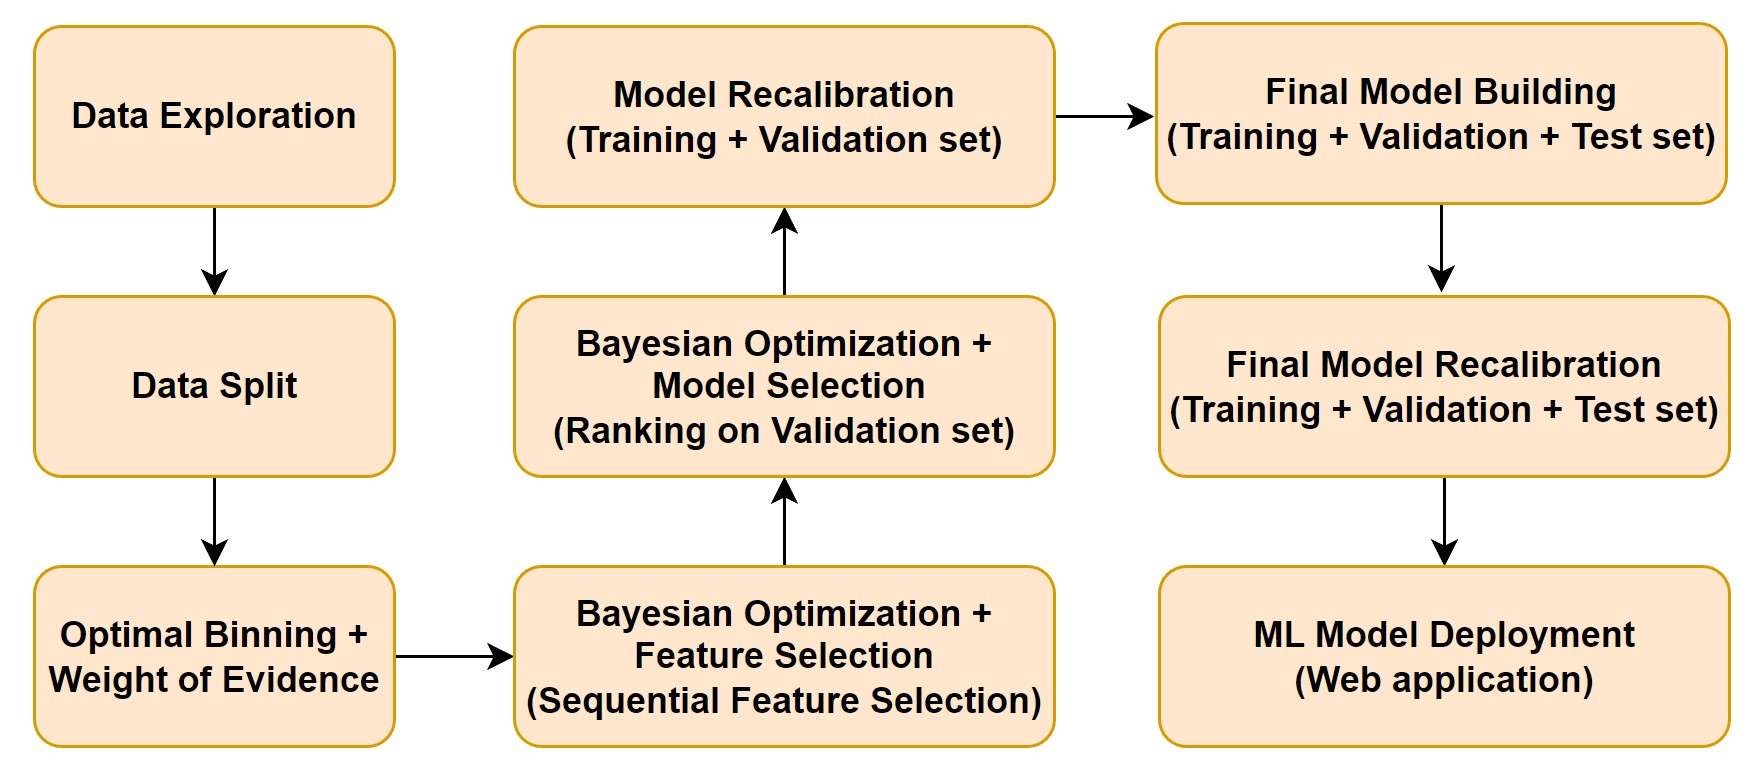
\includegraphics[width=140mm]{Figures/ml_framework.jpg}

\centering{\begin{source}Author's Framework\end{source}}\vspace{-1em}
\end{figure}

\newpage
\section{Repository and Environment Structure}
\label{sec:repo}
The whole machine learning implementation as the scope of this thesis, is developed mainly using Python Programming Language and further with the collaboration of Git and Hypertext Markup Language (HTML).
The whole repository can be found in the separate appendix or is available on the GitHub repository which is accessible via the following link: \url{https://github.com/petr-ngn/FFU_VSE_Masters_Thesis_ML_Credit_Risk_Modelling}.
The repository structure is shown in \autoref{fig:repostructure}.
\begin{figure}[H]
\centering\caption{Repository Structure}
\label{fig:repostructure}

{\footnotesize
\begin{verbatim}
                        |--- data
                        |  |--- interim_dat.csv
                        |  |--- preprocessed_data.csv
                        |  |--- raw_data.csv
                        |
                        |--- flask_app
                        |  |--- inputs
                        |  |  |--- inputs_flask_app_dict.pkl
                        |  |
                        |  |--- templates
                        |  |  |--- index.html
                        |  |  |--- results.html
                        |  |
                        |  |--- static
                        |  |
                        |  |--- app.py
                        |
                        |--- models
                        |  |--- feature_preprocessing
                        |  |--- feature_selection
                        |  |--- model_selection
                        |  |--- objects_FINAL
                        |
                        |--- plots
                        |
                        |--- Masters_Thesis.ipynb
                        |--- requirements.yml
\end{verbatim}
}
\centering{\begin{source}Author's repository at GitHub\end{source}}\vspace{0em}
\end{figure}


\begin{itemize}\setlength\itemsep{0em}
    \item \texttt{data} - Directory containing the raw data, partially preprocessed data (\texttt{interim}) and the final preprocessed data.
    \item \texttt{flask\_app} - Directory containing the Flask application, which is used for the deployment of the model. Particularly, it contains the \texttt{app.py} file, which is the main back-end file of the application, the \texttt{templates} and \texttt{static} subdirectories, which contain the front-end HTML files for the application, and the \texttt{inputs} subdirectory, which contains the input dictionary for the application (such as the trained model, threshold, final features, etc.).
    \item \texttt{models} - Directory containing the sub--directories of the trained and fitted objects for feature preprocessing, feature selection, and model selection, including the final objects used in evaluation and deployment.
    \item \texttt{plots} - Directory containing the plots generated within the main Python notebook.
    \item \texttt{Masters\_Thesis.ipynb} - Main Python notebook containing the main part of the machine learning implementation, such as exploratory analysis, data preprocessing, training, and evaluation of the models. Web application deployment is not included in this notebook, but in \texttt{app.py} Python script.
    \item \texttt{requirements.yml} - File containing the list of the required packages and their specific versions used in this project.
\end{itemize}
    
    

This particular solution is developed in Python version 3.10.9 and these are the main packages and modules used in this project:
\begin{itemize}\setlength\itemsep{0em}
\item \lstinline{NumPy}, \lstinline{Pandas} - for data manipulation and analysis;
\item \lstinline{Matplotlib}, \lstinline{Seaborn} - for data visualization;
\item \lstinline{Scipy} - for statistical analysis;
\item \lstinline{OptBinning} - for optimal binning of features with respect to the target;
\item \lstinline{ImbLearn} - for handling imbalanced data using oversampling;
\item \lstinline{Scikit-learn} - for ML modelling, feature selection, model selection, and model evaluation;
\item \lstinline{Scikit-optimize} - for hyperparameter tuning;
\item \lstinline{Flask} - for deployment of the model as a web application.
\end{itemize}
\newpage
To replicate this solution, one may download this repository as a zip file or clone this repository using Git to the local repository. Before running any files or scripts, it is important to set the environment for such project using the file \texttt{requirements.yml}.
This can be done by running the following command in the Anaconda terminal which will create the new environment with the name \texttt{FFU\_VSE\_Masters\_Thesis} and install all the required packages, as shown in \autoref{fig:envsetup}:
\begin{figure}[H]
    \centering\caption{Environment Setup Command}
    \label{fig:envsetup}
\centering\
{\footnotesize
\begin{verbatim}
    >> conda env create -n FFU_VSE_Masters_Thesis -f requirements.yml    
\end{verbatim}
}
\centering{\begin{source}Author's command at Anaconda\end{source}}\vspace{0em}
\end{figure}
An user should be aware of his current path directory in the terminal. In order to install the file \texttt{requirements.yml}, one needs to define a path to the directory, where such file is located.
To achieve this, the user has to either change the path in the terminal using \texttt{cd} command, insert the path directory before the \texttt{requirements.yml} in terminal, or copy the file \texttt{requirements.yml} to the current path directory. The following code in \autoref{fig:envsetupcd} shows the former approach:
\begin{figure}[H]
    \centering\caption{Environment Setup Command with Directory Change}
    \label{fig:envsetupcd}
\centering\
{\footnotesize
\begin{verbatim}
    >> cd C:\Users\ngnpe\FFU_VSE_Masters_Thesis_ML_Credit_Risk_Modelling
    >> conda env create -n FFU_VSE_Masters_Thesis -f requirements.yml   
\end{verbatim}
}

\centering{\begin{source}Author's command at Anaconda\end{source}}\vspace{0em}
\end{figure}


To preserve the reproducibility of this solution and consistency of the results, the random seed is instantiated to \texttt{42}, so for instance, data split, model optimization, or training would be deterministic and not totally random every time when replicating the solution.
Some \lstinline{Scikit-learn} or \lstinline{Scikit-optimize} objects have the optional argument \texttt{n\_jobs} which utilizes the number of central processing units (CPU) cores used during the parallelizing computation. Such argument is set to \texttt{-1}, hence, all the processors are used in order to speed up the training or optimization process.


\newpage
\section{Data Exploration}
\label{sec:dataexploration}
This section is focused on the exploration of the analyzed loan data set, particularly on data set description, distribution analysis, and association analysis, in order to infer potential valuable insights that can be used in the preprocessing, modelling or evaluation part.

\subsection{Data Set Description}
\label{subsec:datadescript}
The analyzed data set pertains to the HMEQ data set, which contains loan application information and default status of 5,960 US home equity loans. Such data set was acquired from Credit Risk Analytics website \citep{baesens2016credit}. Since this data set regards loan application scoring data, using macroeconomic or other external data is omitted due to the data set's characteristics as well as modelling with behavioral scoring.
Thus, our goal is to predict whether the loan applicant will or will not default based on the information provided in the loan application.
Thus, we aim to predict the probability of default only, therefore, EAD, LGD, and ECL are not considered in this thesis.

As can be seen in \autoref{tab:dataset}, the data set contains 13 columns, 12 features, and 1 target variable, \texttt{BAD} indicating whether the loan was in default (\texttt{1}) or not (\texttt{0}).
Amongst the 12 features, there are 10 numeric features and 2 categorical features, namely \texttt{REASON} which contains 2 categories - Debt consolidation (\texttt{DebtCon}) and Home improvement (\texttt{HomeImp}), and \texttt{JOB} which contains following categories - Administration (\texttt{Office}), Sales, Manager (\texttt{Mgr}), Professional Executive (\texttt{ProfExe}), Self-employed (\texttt{Self}), and Other.

Although all the variables and their names seem to be self-explanatory, one may find the \texttt{DEROG} feature's meaning unclear. In such case, derogatory report refers to the derogatory mark on a credit report, which is the negative item indicating significant credit risk as an indicator of delinquency issues or late payments \citep{experian}. Such credit report is provided by the credit bureau based on the bank's request when assessing the creditworthiness of the loan applicant.


Regarding the indirect data quality issues, the data set's source does not specify the time period of its observations or the snapshot date, which may also be relevant point given that some loans might default after the snapshot date even though they had not defaulted before.
Nevertheless, as already mentioned in introduction, the main goal of this thesis is the implementation of a custom machine learning implementation framework, while the data set is used only as a proof of concept.
Therefore, we deem it appropriate to omit the raised data quality issues in this thesis.

\begin{table}[H]
\small
\setlength{\tabcolsep}{8pt}
\renewcommand{\arraystretch}{1.3}
\centering
\caption[Data Set Variables]{Data Set Variables}\label{tab:dataset}
\begin{tabular}{@{} l p{8cm} l @{}}
\toprule
\textbf{Variable} & \textbf{Description} & \textbf{Data type}\\
\midrule
\hline
BAD & Default status & Boolean \\

LOAN & Requested loan amount & numeric \\

MORTDUE & Loan amount due on existing mortgage & numeric \\

VALUE & Value of current underlying collateral property & numeric \\

REASON & Reason of loan application & categorical \\
JOB & Job occupancy category & categorical \\

YOJ & Years of employment at present job & numeric \\

DEROG & Number of derogatory reports & numeric \\

DELINQ & Number of delinquent credit lines & numeric \\

CLAGE & Age of the oldest credit line in months & numeric \\

NINQ & Number of recent credit inquiries & numeric \\

CLNO & Number of credit lines & numeric \\

DEBTINC & Debt-to-income ratio & numeric \\
\hline
\bottomrule
\end{tabular}
\vspace{0.35em}

\centering{\begin{source}\citep{baesens2016credit}\end{source}}\vspace{-1em}
\end{table}

After the initial data inspection, the data set does not contain any duplicates but does contain missing values, which are summarized in \autoref{tab:natable}.
Most of the missing values are observed within the feature \texttt{DEBTINC} with 1,267 missing observations,
whereas variables indicating default status (\texttt{BAD}) or requested loan amount (\texttt{LOAN}) do not contain any missing values, which is expected as the bank should have the available information about their loans whether they have defaulted or not, and since this data set pertains to the application scoring, when applying for a loan, an applicant should always fill out the requested loan amount.

\begin{table}[H]
\small
\setlength{\tabcolsep}{8pt}
\renewcommand{\arraystretch}{1.3}
\centering
\caption[Missing Values Summary]{Missing Values Summary}\label{tab:natable}
\begin{tabular}{l r r}
\toprule
\textbf{Variable} & \textbf{\# NA's} & \textbf{\% NA's}\\
\midrule
\hline
BAD & 0 & 0.00 \% \\
LOAN & 0 & 0.00 \% \\
MORTDUE & 518 & 8.69 \% \\
VALUE & 112 & 1.88 \% \\
REASON & 252 & 4.23 \% \\
JOB & 279 & 4.68 \% \\
YOJ & 515 & 8.64 \% \\
DEROG & 708 & 11.88 \% \\
DELINQ & 580 & 9.73 \% \\
CLAGE & 308 & 5.17 \% \\
NINQ & 510 & 8.56 \% \\
CLNO & 222 & 3.72 \% \\
DEBTINC & 1267 & 21.26 \% \\
\hline
\bottomrule
\end{tabular}
\vspace{0.35em}

\centering{\begin{source}Author's results in Python\end{source}}\vspace{-1em}
\end{table}


\subsection{Distribution Analysis}
\label{subsec:distribution}
In this subsection, we inspect the distribution of our variables, including the target variable and the features.
Such distribution inspection may help us identify outliers, and other potential issues with the data set.

\subsubsection{Default Distribution}
\label{subsubsec:defaultdist}

Regarding the target variable distribution, from the \autoref{fig:defaultdist} we can observe that the default status distribution is heavily imbalanced, as most of the loans have not defaulted yet.
Particularly, 80.05\% of the observations have been labeled as non-default (4,771 observations) and 19.95\% observations labeled as default (1,189 observations).
This may cause problems in the modelling part, as the model might be biased towards the majority class, i.e., the non-default class. Such imbalanced class issue will be further treated in \autoref{subsec:data-split-ADASYN}.

\begin{figure}[H]
\centering
\caption{Default Distribution}
\label{fig:defaultdist}
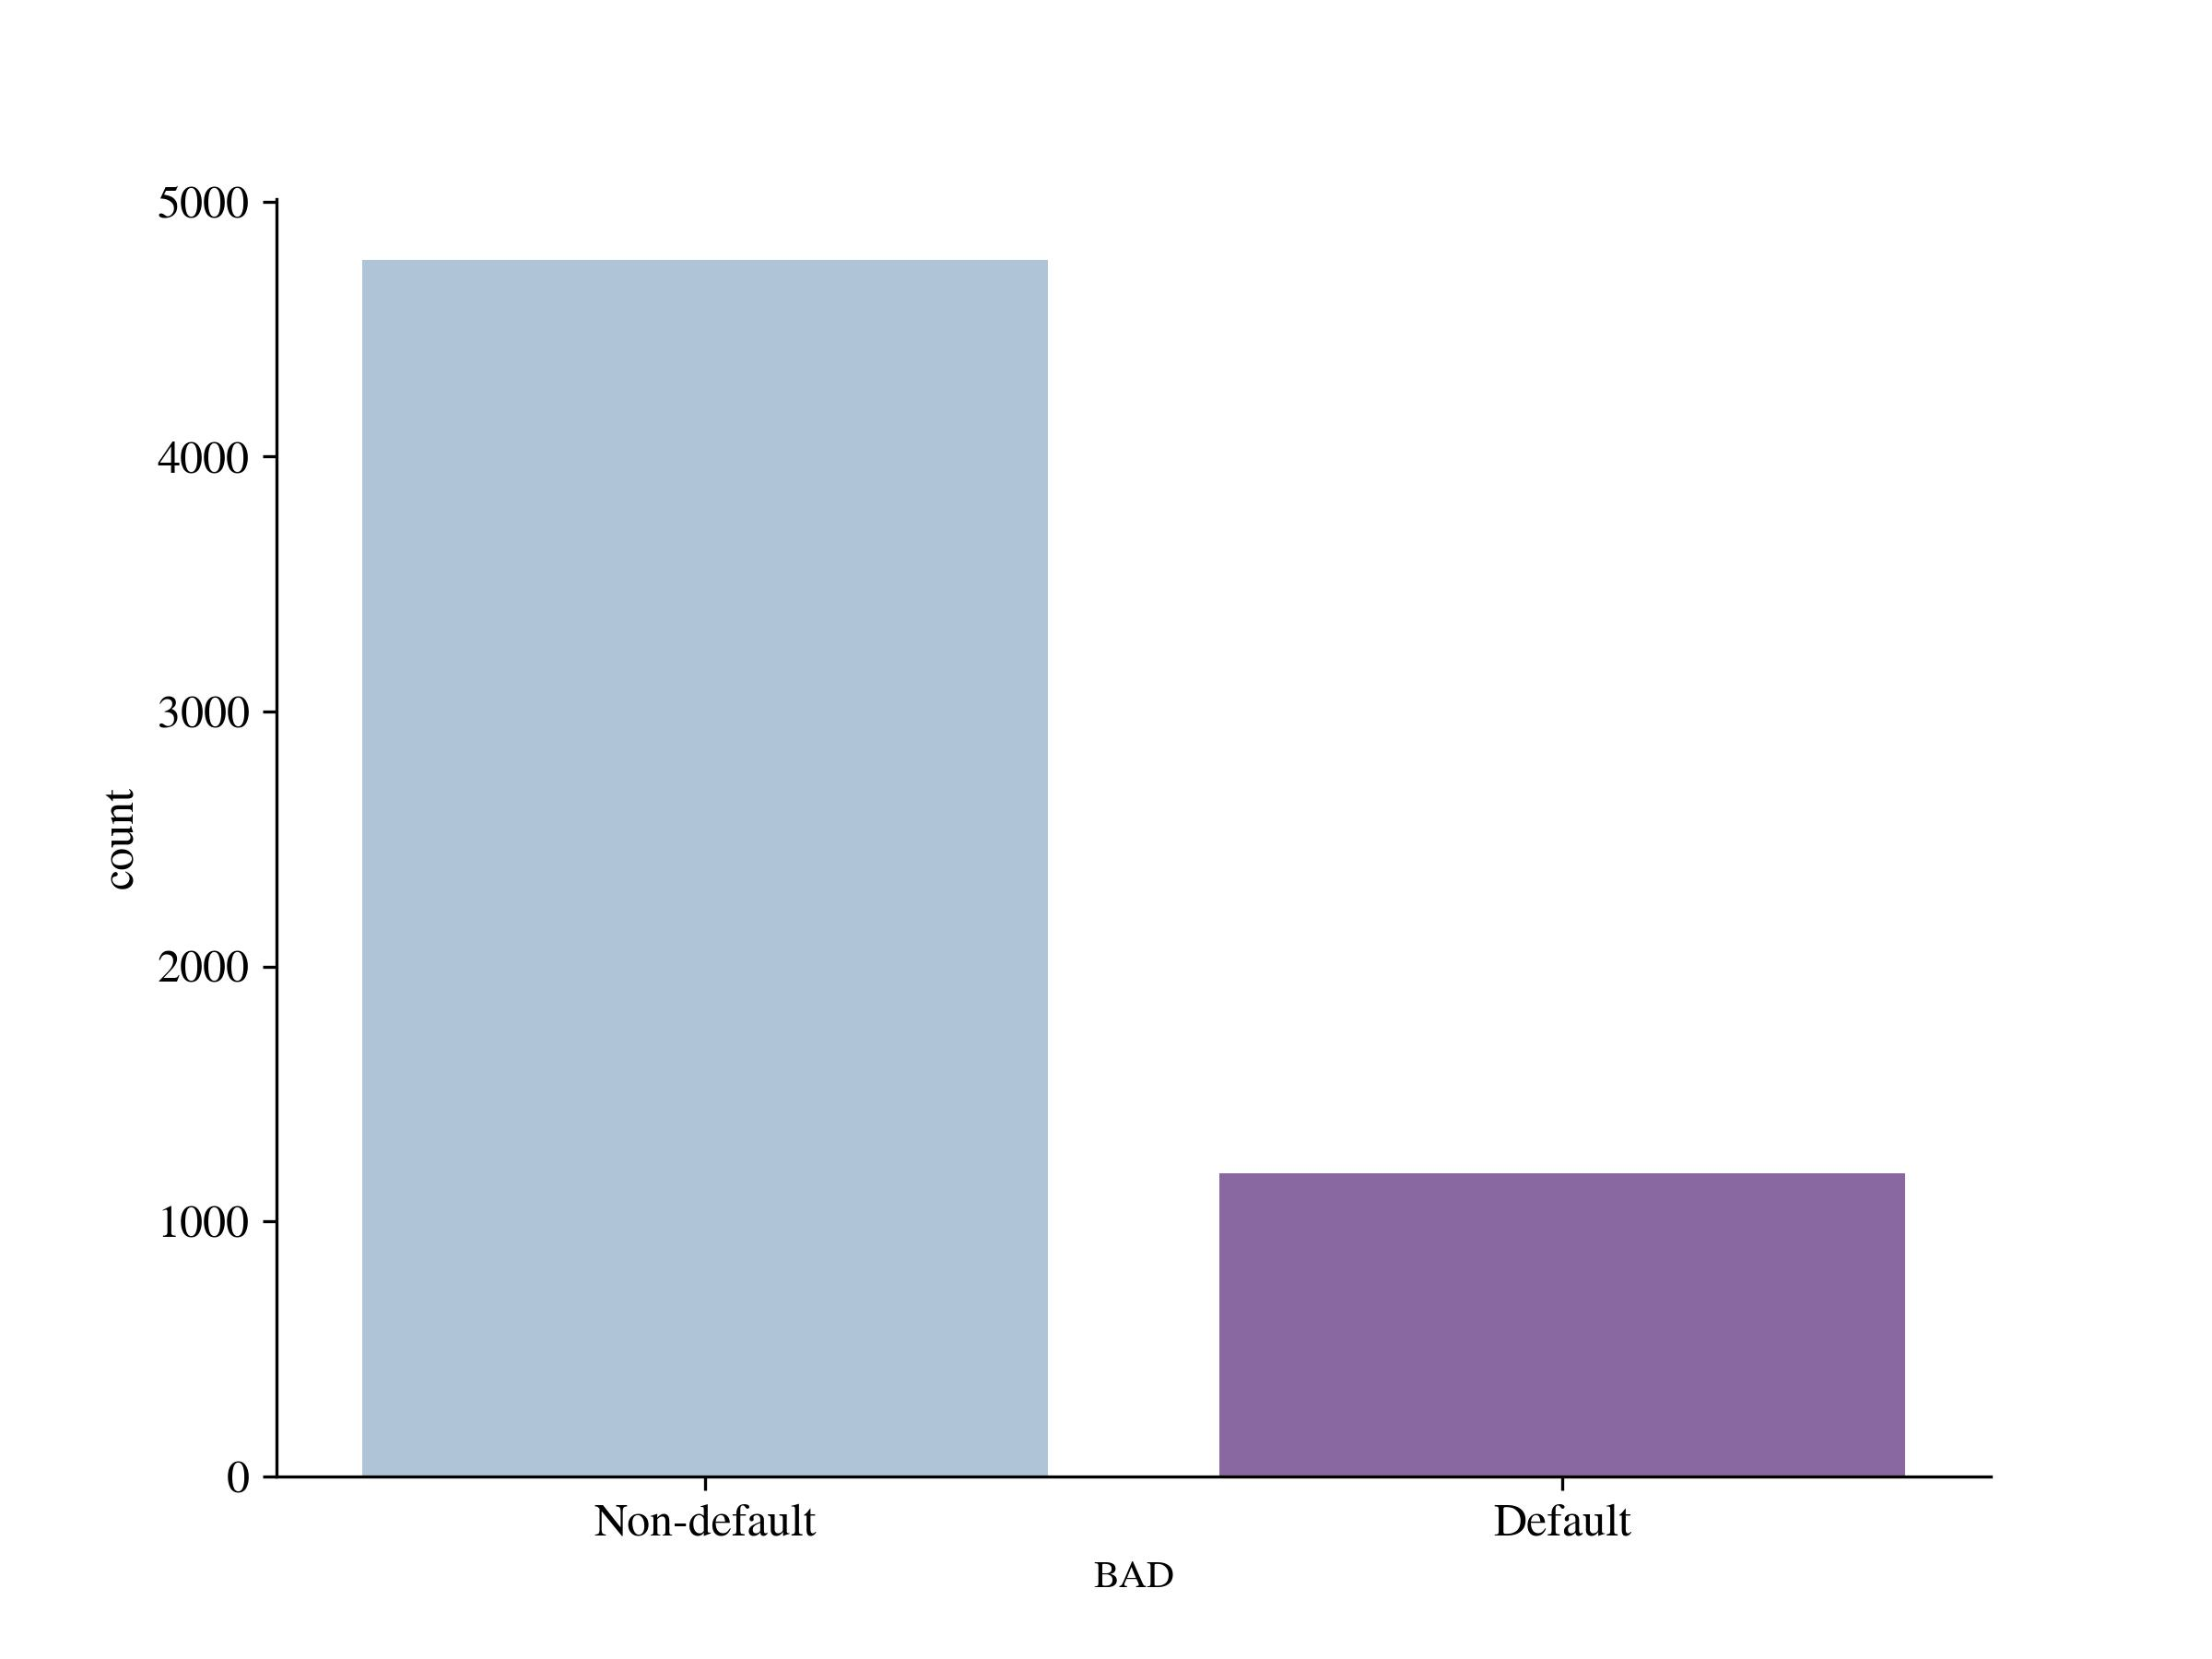
\includegraphics[width=130mm]{Figures/Default_Distribution.jpg}\vspace{-1em}

\centering{\begin{source}Author's results in Python\end{source}}\vspace{-1em}
\end{figure}

\subsubsection{Numeric Features' Distribution}
\label{subsubsec:numdist}

Regarding the numeric features, it can be observed that most of them exhibit a positive skewness and contain outliers, as illustrated in \autoref{fig:boxfeat}, which depicts the conditional distribution of the numeric features with respect to the default status via boxplots.
All the outliers appear to be valid, indicating that they have not arisen due to data entry errors.
This can be attributed to the non-negative nature of all the numeric features, which makes it impossible to have negative values for features such as the number of years at the present job or the number of delinquent credit lines, among others.
Additionally, the maximum values of the given features are not unrealistically high, further corroborating the validity of the outliers.


However, it is necessary to treat these outliers as such, as they can bias and jeopardize the model's weights, coefficients, or distance calculation, which may significantly affect the position and orientation of the decision boundary.
Such factors can lead to overfitting, inaccurate, and biased predictions.
A detailed explanation of the outlier treatment is provided in \autoref{subsec:prep-optbinning}.


\newpage
Concerning the target variable, it can be observed that there are some differences in the distribution shapes of \texttt{DEROG} and \texttt{DELINQ}, which exhibit less skewness and lower dispersion for non-default cases as compared to default cases.
Since both features indicate negative information about delinquency, it is expected that a higher value for these features would increase the likelihood of loan default.
Referring to the feature \texttt{DEBTINC}, it does not exhibit any extreme values for non-default cases, but some extreme values are present for default cases.
From this, it can be inferred that if the debt-to-income ratio is too high, indicating that the applicant's income is not sufficient to cover their debt, the loan is more likely to end in default.
The association between the default status and the numeric features is further investigated in \autoref{subsubsec:target-num-ass}.


Since the features are substantially positively skewed, they do not follow a Gaussian (normal) distribution. Additionally, Shapiro--Wilk test is conducted in order to assess whether the features' distributions are significantly different from the normal distribution.
According to such test, all the numeric features' distributions do not follow the normal distribution on 1\% statistical significance level.
For a reference, see \autoref{tab:normalitytest} in \autoref{chap:app1}.


\begin{figure}[H]
\centering
\caption{Conditional Distribution of Numeric Features}\vspace{0.5em}
\label{fig:boxfeat}
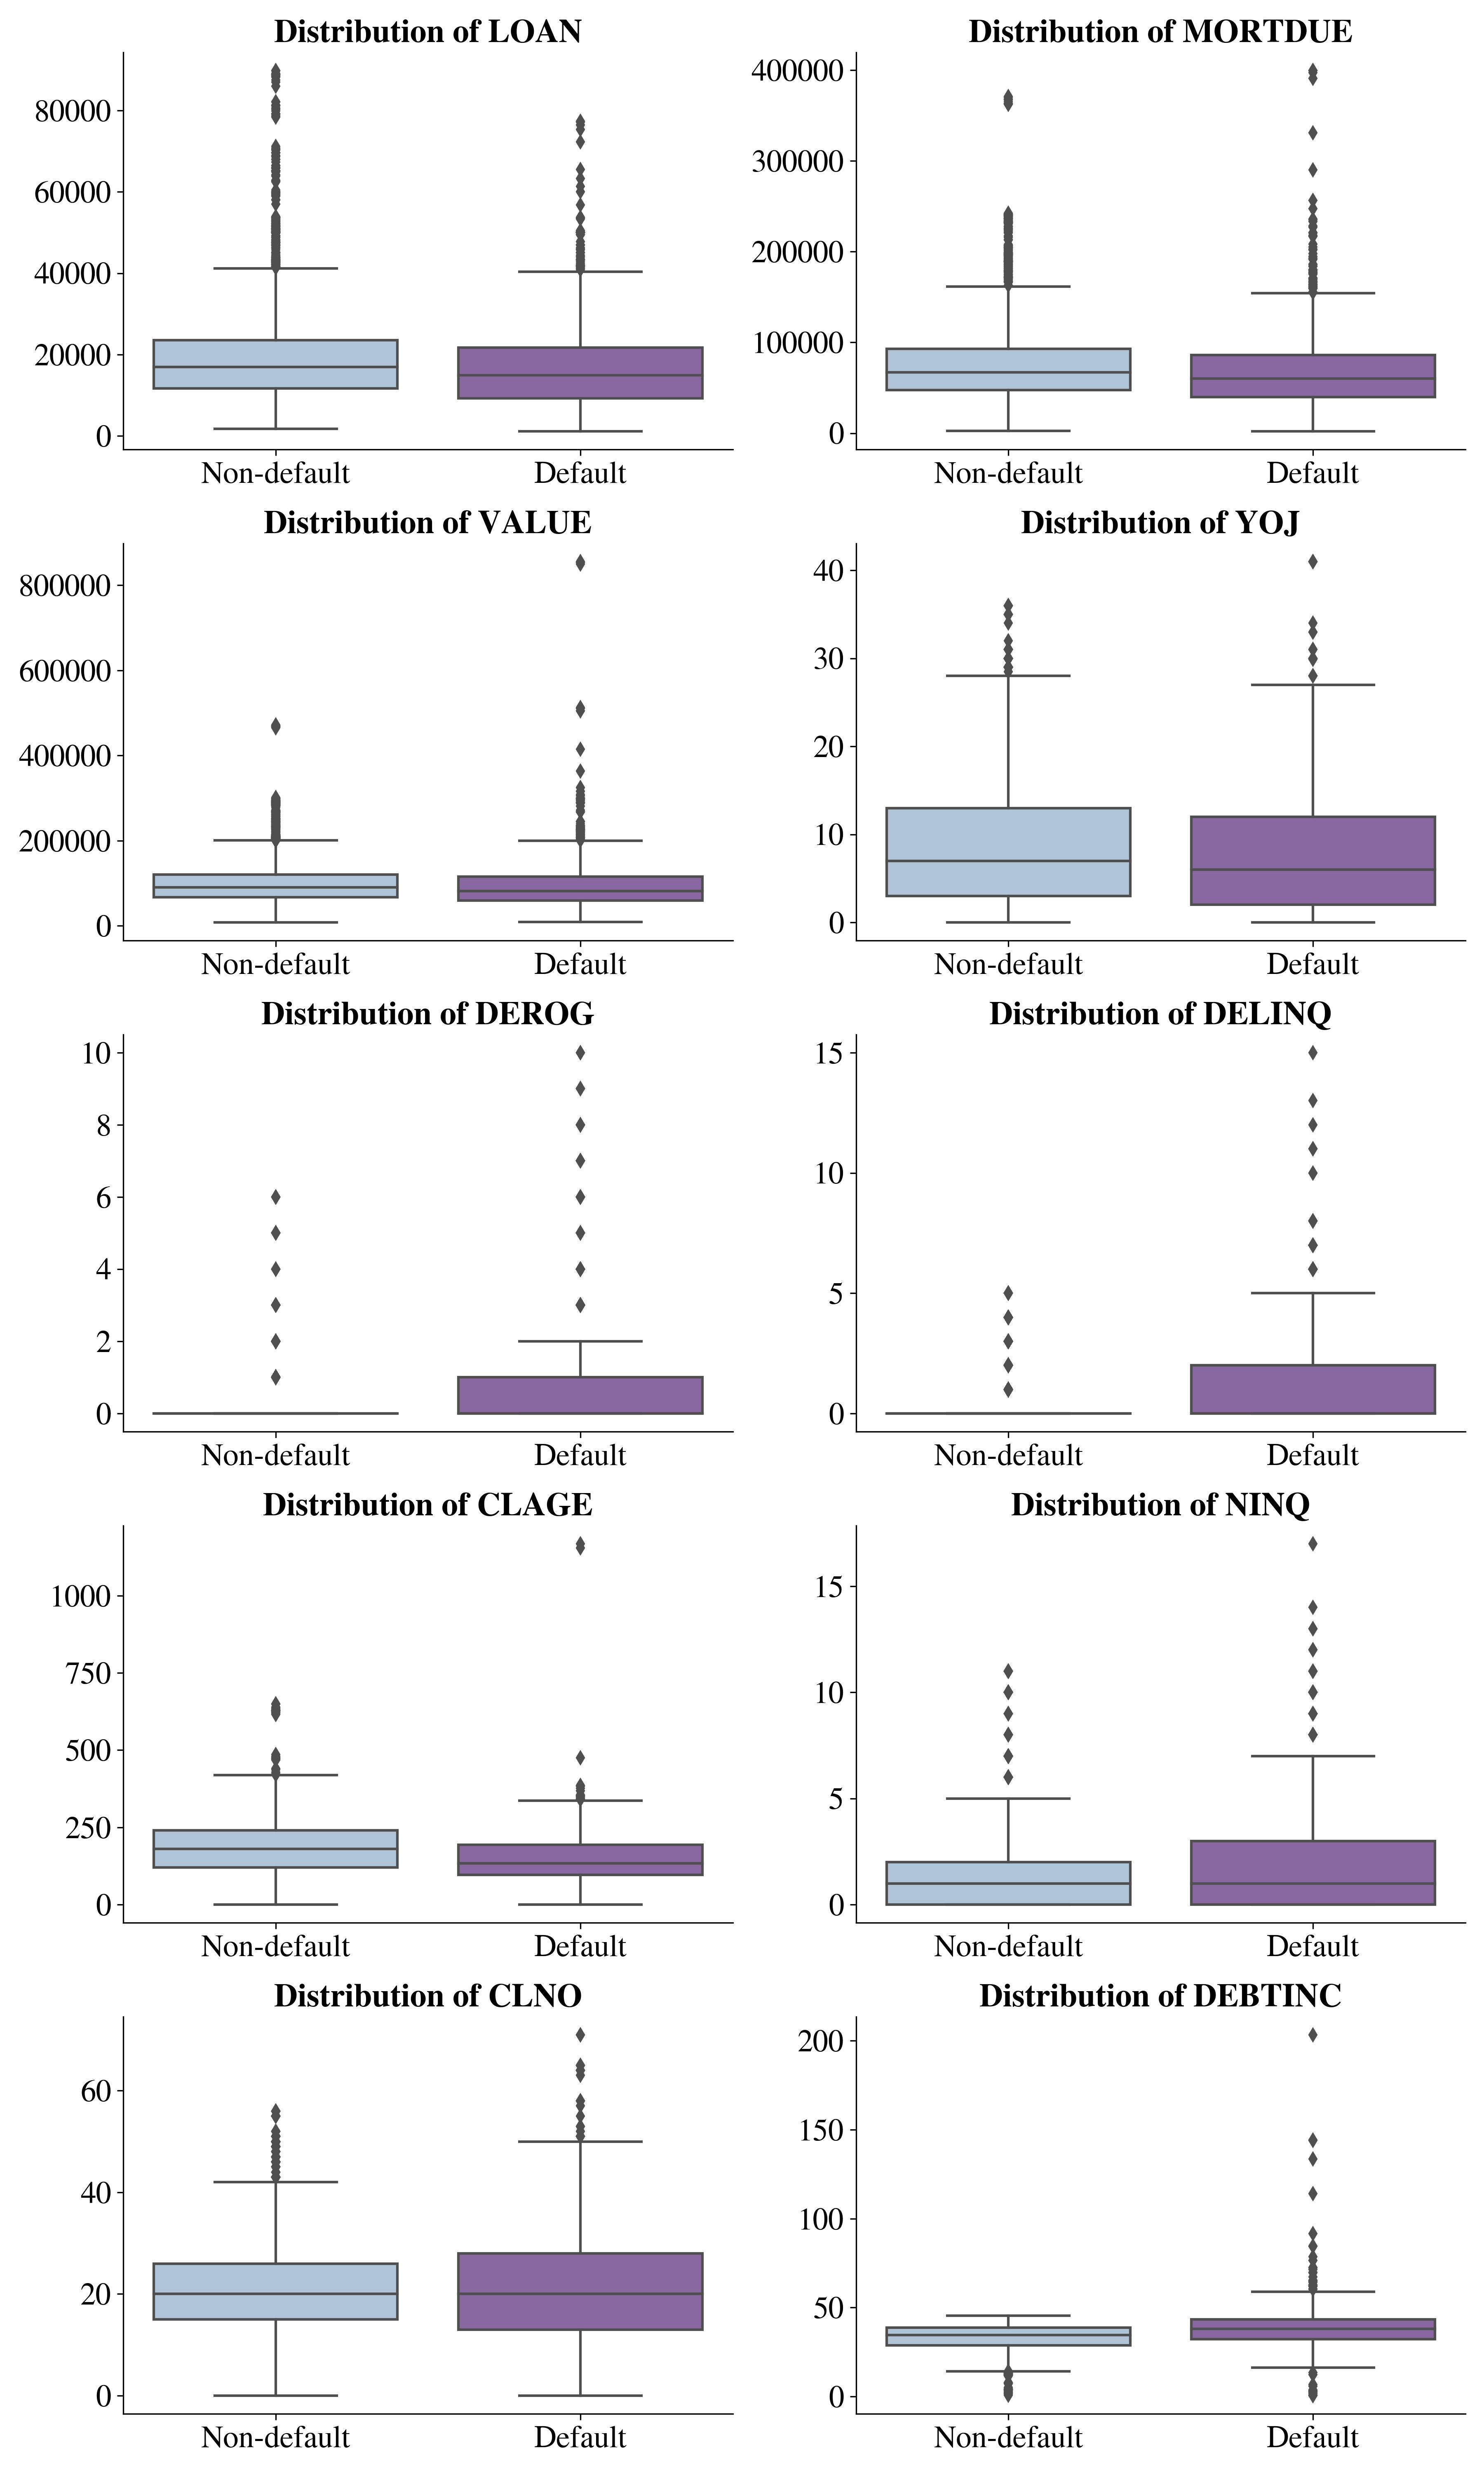
\includegraphics[width=140mm]{Figures/Numeric_Features_Distribution_Boxplots.jpg}

\centering{\begin{source}Author's results in Python\end{source}}\vspace{-1em}
\end{figure}

Due to the fact that the boxplots do not capture the missing values that occurred in given features, it is also important to inspect the numbers and proportions of missing values in each feature, conditional on the default status.
As can be seen in \autoref{tab:nacont-table}, $n_0$ refers to the number of missing values in the given feature for non-default cases, and $n_1$ refers to the number of missing values in the given feature for default cases.
$N_0$ and $N_1$ refer to the total number of non--default cases and default cases, respectively, therefore, $n_0/N_0$ refers to the proportion of missing values in the given feature for non-default cases, and $n_1/N_1$ refers to the proportion of missing values in the given feature for default cases.


Pertaining to the feature \texttt{DEBTINC}, we can observe a significant difference in the number of missing values between the default and non-default cases. Out of all defaulted loans, 66.11 \% had a missing debt--to--income ratio, whereas only 10.08 \% out of all non-defaulted loans had a missing debt--to--income ratio.
Therefore, there could be a strong association between the missing debt--to--income ratio and the default.


Similarly, the table depicts a significant difference with respect to \texttt{VALUE} as 0.15 \% had missing collateral property value out of all non--defaulted loans and 8.92 \% defaulted loans had missing collateral property value.
It can be inferred that loan applicants who withhold information on their collateral property value or debt-to-income ratio are more likely to default on their loans.
This may be due to negative information that they are trying to conceal, such as excessively high debt, low income, or a low collateral property value.
Such associations are further investigated in \autoref{subsubsec:target-na-ass}.


\begin{table}[H]
\small
\setlength{\tabcolsep}{8pt}
\renewcommand{\arraystretch}{1.3}
% define a new column type 'L' for left alignment
\newcolumntype{R}[1]{>{\raggedleft\arraybackslash}p{#1}} % define a new column type 'R' for right alignment
\begin{center}
\caption[Numeric Features NA's Summary]{Numeric Features NA's Summary}\label{tab:nacont-table}
\begin{tabular}{l R{1cm}R{1cm}|R{1.5cm}R{1.5cm}}
    \toprule
    \textbf{Feature} & \textbf{$n_0$} & \textbf{$n_1$} & \textbf{$n_0/N_0$} & \textbf{$n_1/N_1$} \\
    \midrule
    \hline
    LOAN & 0 & 0 & 0 \% & 0 \% \\

    MORTDUE & 412 & 106 & 8.64 \% & 8.92 \% \\

    VALUE & 7 & 105 & 0.15 \% & 8.83 \% \\

    YOJ & 450 & 65 & 9.43 \% & 5.47 \% \\

    DEROG & 621 & 87 & 13.02 \% & 7.32 \% \\

    DELINQ & 508 & 72 & 10.65 \% & 6.06 \% \\

    CLAGE & 230 & 78 & 4.82 \% & 6.56 \% \\

    NINQ & 435 & 75 & 9.12 \% & 6.31 \% \\

    CLNO & 169 & 53 & 3.54 \% & 4.46 \% \\

    DEBTINC & 481 & 786 & 10.08 \% & 66.11 \% \\ \hline
    \bottomrule
\end{tabular}
\end{center}
\begin{center}

\source{Author's results in Python}
\end{center}
\end{table}
\subsubsection{Categorical Features' Distribution}
\label{subsubsec:catdist}

Regarding the distribution of categorical features, the data set includes 2 nominal features, namely \texttt{REASON} and \texttt{JOB}.
The conditional distribution of categorical features on the default status is visualized using barplots in \autoref{fig:catdist}.
The plot indicates that most loan applicants applied for debt consolidation, while most job occupancies were labeled as \texttt{Other}.

With respect to the default status, there appears to be no strong difference between the default and non-default cases in terms of the relative distribution of the \texttt{REASON} feature.
However, a slight difference is observed between the default and non-default cases in terms of the relative distribution of the \texttt{JOB} feature.
Specifically, the categories \texttt{Office}, \texttt{ProfExe}, and \texttt{N/A} exhibit a relatively higher proportion of non-default cases than default cases.
Hence, a moderate association between the \texttt{JOB} feature and the default status is possible, as further investigated in \autoref{subsubsec:target-cat-ass}.



\begin{figure}[H]
\centering
\caption{Conditional Distribution of Categorical Features}\vspace{0.5em}
\label{fig:catdist}
\includegraphics[width=140mm]{Figures/Categorical_Features_Distribution.jpg}

\centering{\begin{source}Author's results in Python\end{source}}\vspace{-1em}
\end{figure}
\subsection{Association Analysis}
\label{subsec:assanal}
In this subsection, we aim to examine potential relationships between the variables by analyzing their associations. Firstly, we investigate the association between the default status and the features. Subsequently, we explore the associations among the features themselves.

\subsubsection{Association between Default Status and Numeric Features}
\label{subsubsec:target-num-ass}

To measure the association between the target variable and the numeric features, we use the Point-Biserial correlation coefficient, which is the Pearson's product moment correlation coefficient between a continuous variable and a dichotomous variable \citep{kornbrot2014point}.
This coefficient ranges from -1 to +1 and can be used to assess the strength and direction of the relationship between a continuous variable and a binary variable.
The formula for computing this coefficient is as follows:

\begin{equation}\label{eq}
r_{pb,X} =  \frac{\mu \left( X | Y=1 \right) -\mu \left( X | Y=0 \right)}{\sigma_{X}}\sqrt{\frac{N\left(Y=1\right) \times N\left(Y=0\right)}{N \left(N - 1 \right)}}
\end{equation}

where $\mu \left( X | Y=1 \right)$ and $\mu \left( X | Y=0 \right)$ represent the means of the given numeric feature $X$ conditional on the default status and non-default status, respectively, while $\sigma_{X}$ denotes the standard deviation of $X$.
The values of $N\left(Y=1\right)$ and $N\left(Y=0\right)$ indicate the number of observations with default status and non-default status, respectively, and $N$ represents the total number of observations within the feature $X$.


The following \autoref{tab:pointbi} displays the computed Point-Biserial coefficient for each numeric feature with respect to the default status, along with its statistical significance.
The results show that features such as \texttt{DEROG}, \texttt{DELINQ}, and \texttt{DEBTINC} are moderately and positively associated with the default status at the 1\% statistical significance level.
These findings support the observations made in \autoref{subsubsec:numdist} regarding the positive associations of these features with the default status. It can be inferred that these features may serve as important predictors in the model.

\begin{table}[H]
    \small
    \setlength{\tabcolsep}{8pt}
    \renewcommand{\arraystretch}{1.3}
    \centering
        \caption[Point--Biserial Correlation - Numeric Features vs. Default]{Point--Biserial Correlation - Numeric Features vs. Default}\label{tab:pointbi}
        \begin{tabular}{@{} l r @{\hspace{1cm}} l @{{}}}
    \toprule
    \textbf{Feature} & \textbf{Coefficient} & \textbf{Significance}\\
    \midrule
    \hline

    LOAN & -0.075  & ***\\

    MORTDUE & -0.048  & ***\\

    VALUE & -0.030  & ** \\
    
    YOJ & -0.060  & *** \\

    DEROG & 0.276 & *** \\

    DELINQ & 0.354 & *** \\
    
    CLAGE & -0.170 & *** \\

    NINQ & 0.175 & *** \\

    CLNO & -0.004 & \\

    DEBTINC & 0.200 & *** \\
    \hline
    \bottomrule
    \end{tabular}
    \vspace{0.35em}


        \centering\footnotesize{$^{*}$: $p<0.10$, $^{**}$: $p<0.05$, $^{***}$: $p<0.01$}\vspace{0.7em}

        \centering{\begin{source}Author's results in Python\end{source}}\vspace{-1em}

\end{table}

\subsubsection{Association between Default Status and Categorical Features}
\label{subsubsec:target-cat-ass}

In order to measure the strength of the relationship between the dichotomous default status and categorical variables, we employ Cramer's V, which ranges from 0 to 1 and is defined as:


\begin{equation}\label{eq}
    CV_{X} = \sqrt{\frac{\chi^{2}}{N\left(k-1\right)}}
\end{equation}


As noted in \autoref{subsubsec:catdist}, the association between the default status and \texttt{REASON} is weak, as evidenced by the Cramer's V value being close to zero.
Conversely, the association between the default status and \texttt{JOB} is slightly stronger, as the categories \texttt{Office}, \texttt{ProfExe}, and \texttt{N/A} exhibit a higher proportion of non-default cases than default cases.
Both \texttt{REASON}'s and \texttt{JOB}'s associations with default status are statistically significant at the 1\% significance level.

While statistical significance is important, it does not necessarily indicate that a feature is a strong predictor of the target variable.
Ultimately, the usefulness of a feature in predicting the target variable is determined by the performance metrics of the model.

    \begin{table}[H]
        \small
        \setlength{\tabcolsep}{8pt}
        \renewcommand{\arraystretch}{1.3}
        \centering
            \caption[Cramer's V Association - Categorical Features vs. Default]{Cramer's V Association - Categorical Features vs. Default}\label{tab:cramer-v}
            \begin{tabular}{@{} l r @{\hspace{1cm}} l @{}}
        \toprule
        \textbf{Feature} & \textbf{Coefficient} & \textbf{Significance}\\
        \midrule
        \hline
        REASON & 0.038  & ***\\
        JOB & 0.120  & ***\\
        \hline
        \bottomrule
    \end{tabular}
    \vspace{0.35em}


        \centering\footnotesize{$^{*}$: $p<0.10$, $^{**}$: $p<0.05$, $^{***}$: $p<0.01$}\vspace{0.7em}

        \centering{\begin{source}Author's results in Python\end{source}}\vspace{-1em}
\end{table}

\newpage
\subsubsection{Association between Default Status and Missing Values}
\label{subsubsec:target-na-ass}

Given that the loan data set contains missing values, it is necessary to examine whether the missingness is associated with the default status. One possible approach is to encode the feature with missing values as a binary variable, where 1 indicates the presence of a missing value and 0 otherwise.

To quantify the strength of association between the two binary variables, the Phi coefficient is used, which is defined as:

\begin{equation}\label{eq}
\phi_{X} = \sqrt{\frac{\chi^{2}}{n}}
\end{equation}

In line with the finding regarding the \texttt{DEBTINC} and \texttt{VALUE} in \autoref{subsubsec:numdist}, there is a strong and statistically significant association between the missing debt-to-income ratio and default status, and a moderate and statistically significant association between the missing collateral property value and default status, as shown in \autoref{tab:phi-target}.
Therefore, we can anticipate that these features will be crucial indicators in default prediction. Further details on feature selection are presented in \autoref{subsec:feature-selection}.
\begin{table}[H]
    \small
    \setlength{\tabcolsep}{8pt}
    \renewcommand{\arraystretch}{1.3}
    \centering
        \caption[Phi Correlation Coefficient - NA's vs. Default]{Phi Correlation Coefficient - NA's vs. Default}\label{tab:phi-target}
        \begin{tabular}{@{} l r @{\hspace{1cm}} l @{}}
    \toprule
    \textbf{Feature} & \textbf{Coefficient} & \textbf{Significance}\\
    \midrule
    \hline
    LOAN & 0.000  & \\

    MORTDUE & 0.003  & \\
 
    VALUE & 0.254  & *** \\

    REASON & 0.004 & \\

    JOB & 0.064 & *** \\

    YOJ & 0.056  & *** \\

    DEROG & 0.070 & *** \\

    DELINQ & 0.061 & *** \\

    CLAGE & 0.030 & ** \\

    NINQ & 0.039 & *** \\

    CLNO & 0.018 & \\

    DEBTINC & 0.547 & *** \\
    \hline
    \bottomrule
    \end{tabular}
    \vspace{0.35em}


        \centering\footnotesize{$^{*}$: $p<0.10$, $^{**}$: $p<0.05$, $^{***}$: $p<0.01$}\vspace{0.7em}

        \centering{\begin{source}Author's results in Python\end{source}}\vspace{-1em}
\end{table}

\subsubsection{Missing Values Association}
\label{subsubsec:naass}
Additionally, it is imperative to investigate the relationship between missing values and default status, as well as the interrelationship between the missing values themselves.
A common approach to identifying patterns of missing data in a data set is through the use of a dendrogram, which clusters variables hierarchically based on the occurrence of missing values.
This method groups variables into clusters based on the similarity of their missing value patterns, such that variables with comparable patterns of missingness are clustered together.
The dendrogram is constructed by merging the two closest clusters iteratively until all variables are in the same cluster.
The distance between the clusters at each step of the merging is shown on the y-axis of the dendrogram, and the order in which the variables are merged is displayed on the x-axis.

In \autoref{fig:dendrogram}, the hierarchical clustering of the data set's variables is illustrated, excluding the default status and requested loan amount feature \texttt{LOAN}, as these variables do not contain any missing values.
As depicted in the dendrogram, the \texttt{CLNO} and \texttt{CLAGE} features have the most similar patterns of missing value occurrences.
Therefore, it can be inferred that a significant number of loan applicants tend to omit information regarding their number of credit lines (\texttt{CLNO}) and the age of their most recent credit line (\texttt{CLAGE}) when submitting their loan applications.

\begin{figure}[H]
    \centering
    \caption{Nullity Dendrogram}\vspace{0.5em}
    \label{fig:dendrogram}
    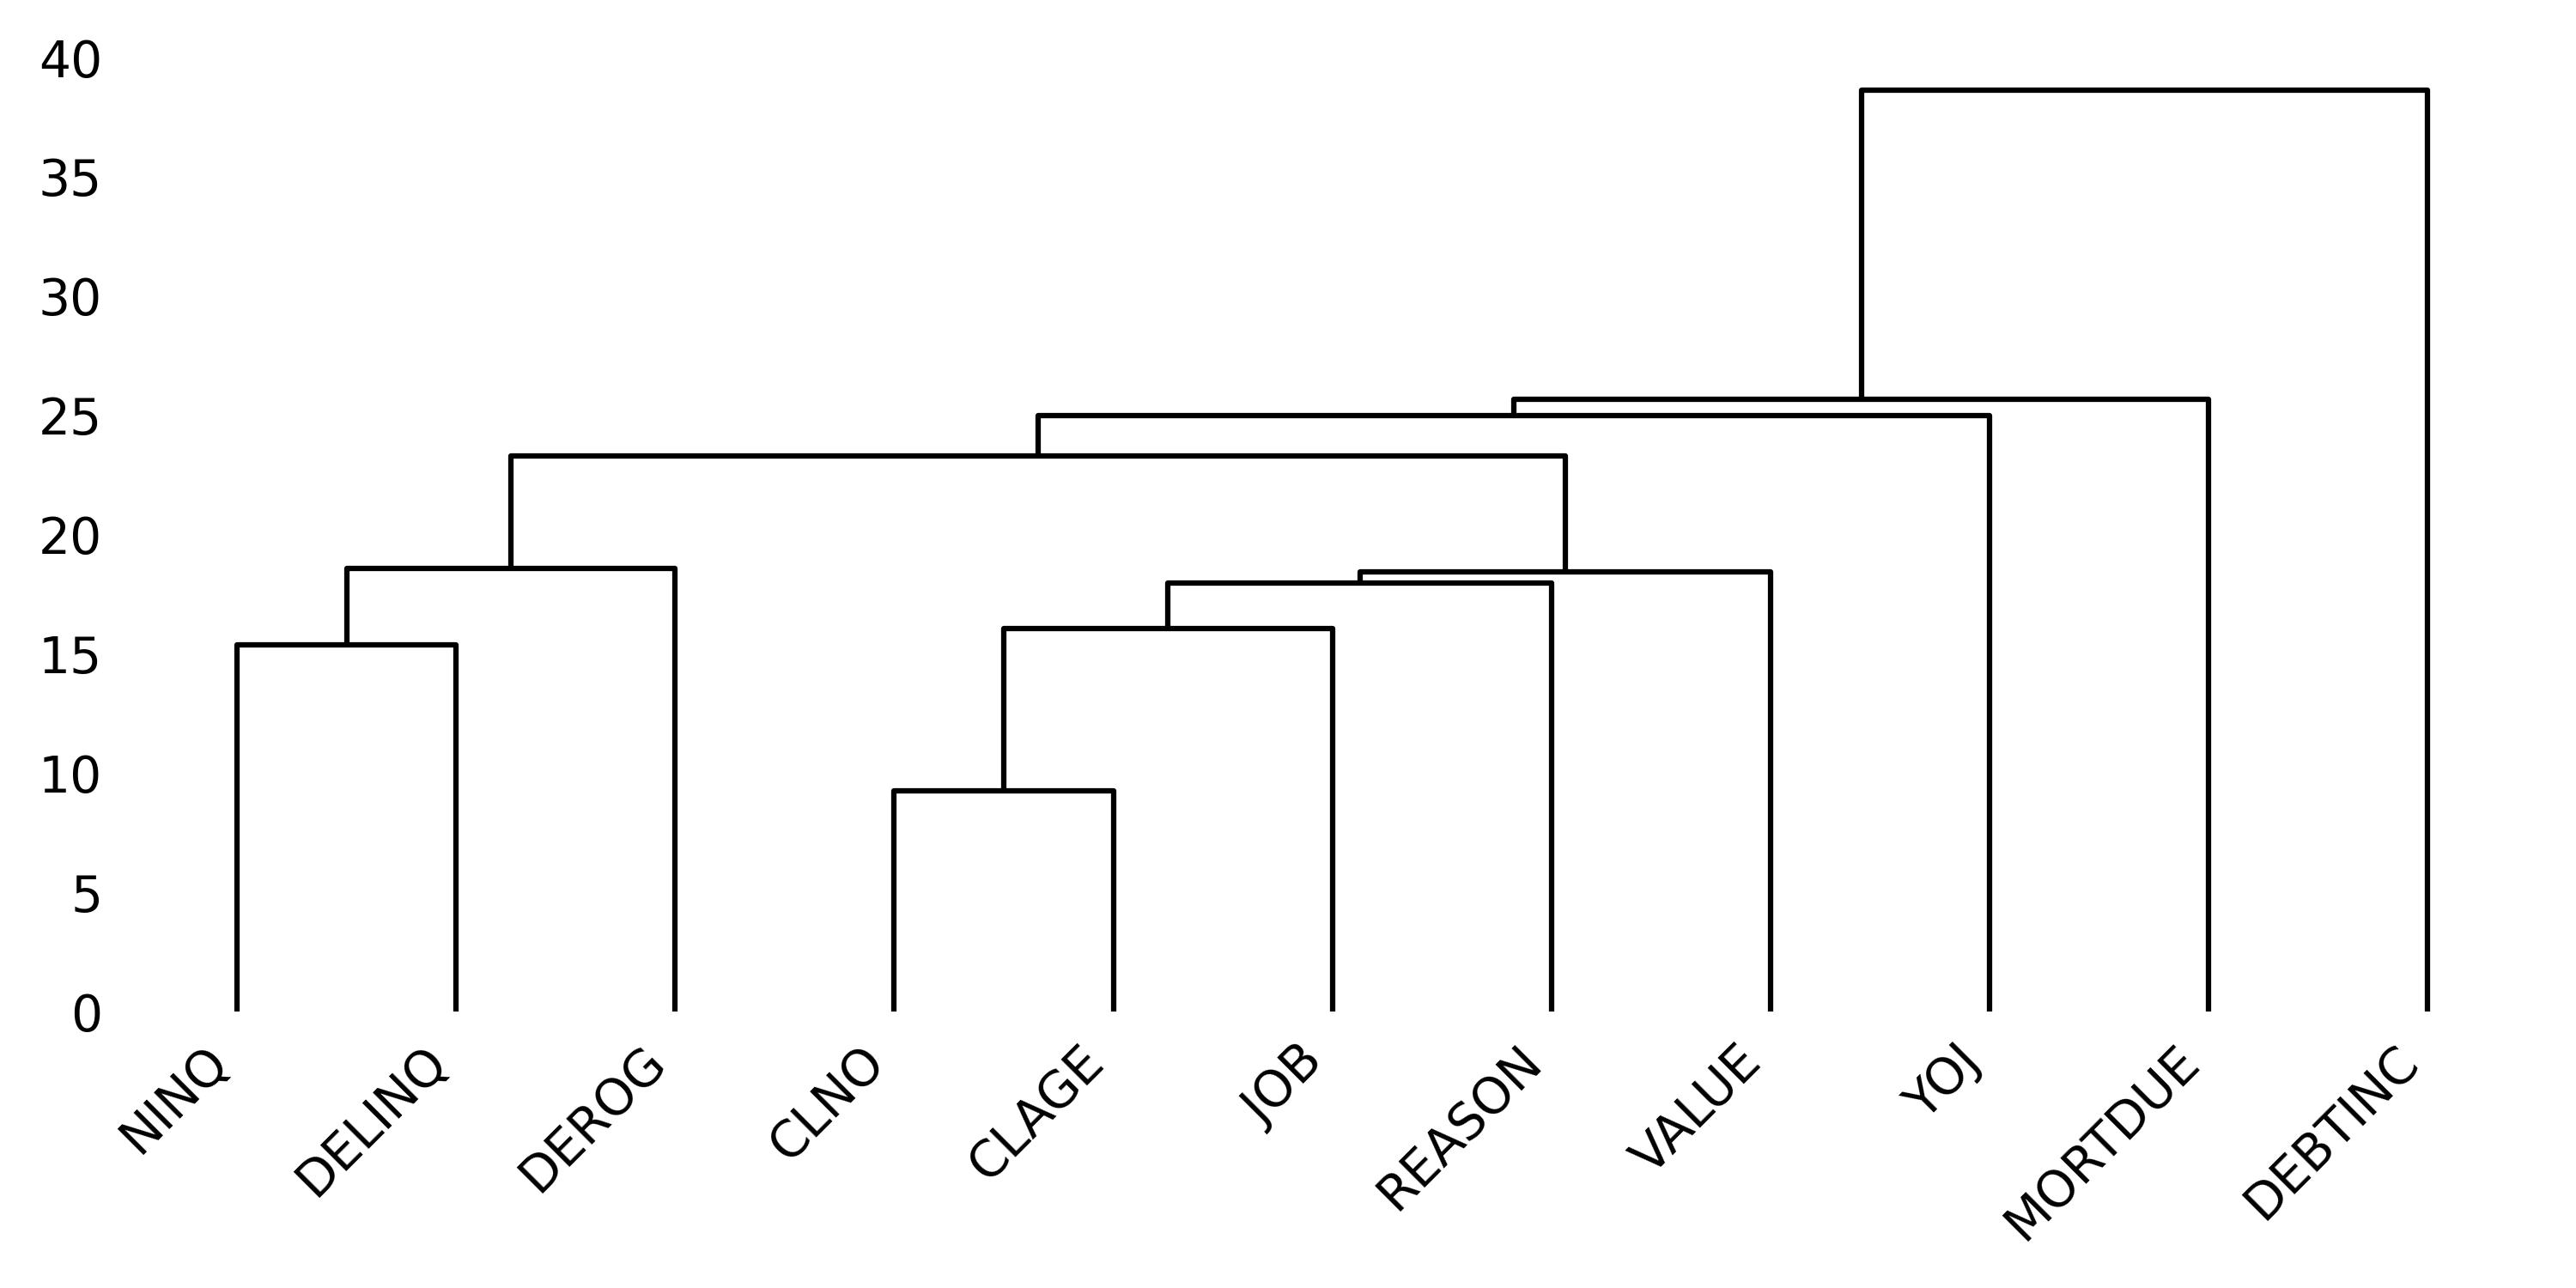
\includegraphics[width=140mm]{Figures/NA_Dendrogram.jpg}

    \centering{\begin{source}Author's results in Python\end{source}}\vspace{-1em}
\end{figure}

Note that the target variable is imbalanced, therefore, the dendrogram depicted in \autoref{fig:dendrogram} is not representative for the default cases. Therefore, we can also inspect the dendrogram for the default cases only, as shown in \autoref{fig:dendrogramdef}.
As can be seen, the hierarchy has changed compared the hierarchy in \autoref{fig:dendrogram}. It can be observed that a significant number of loan applicants tend to omit information regarding their number of credit lines (\texttt{CLNO}) and the number of delinquent credit lines (\texttt{DELINQ}) when submitting their loan applications. Especially regarding the second feature, this might indicate a common delinquency problem among the applicants and, thus, a higher probability of default.
\begin{figure}[H]
    \centering
    \caption{Nullity Dendrogram (default cases)}\vspace{0.5em}
    \label{fig:dendrogramdef}
    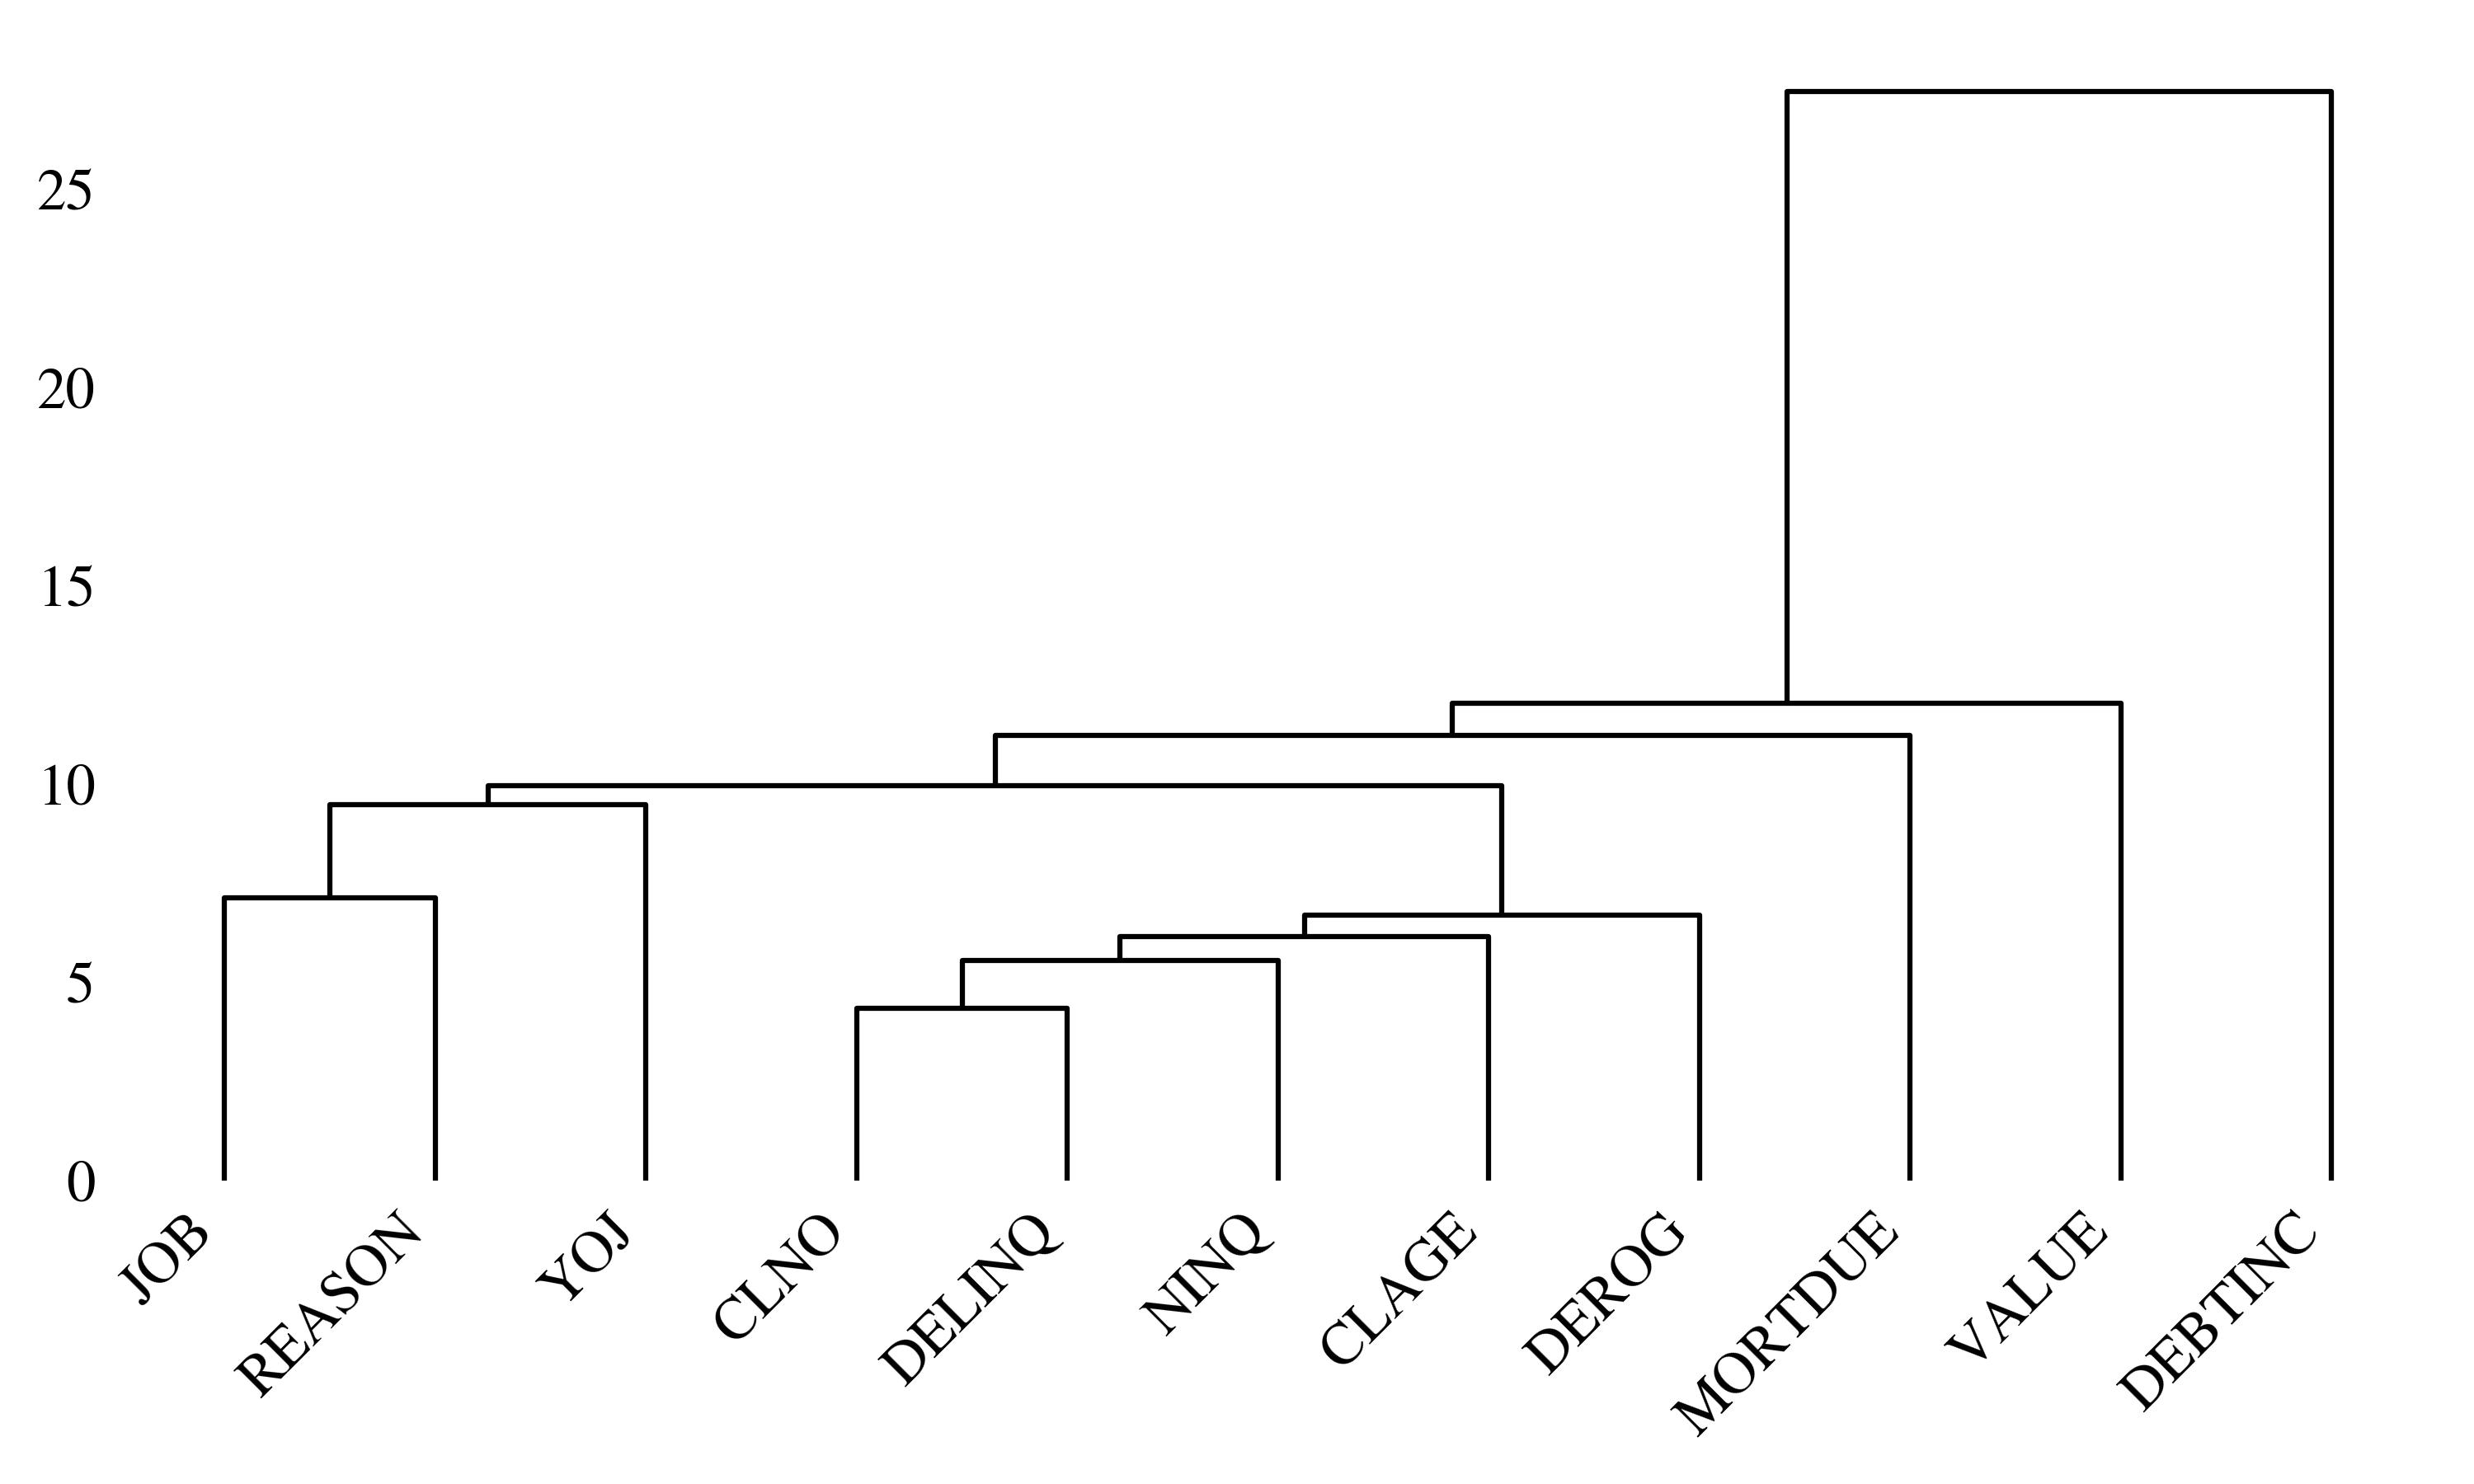
\includegraphics[width=140mm]{Figures/NA_Dendrogram_defaults.jpg}

    \centering{\begin{source}Author's results in Python\end{source}}\vspace{-1em}
\end{figure}

\subsubsection{Multicolinearity Analysis}
\label{subsubsec:multicolinearity}
To quantify the association between the numerical features, the Pearson correlation coefficient is often used.
However, it is highly sensitive to outliers and makes assumptions regarding the normal distribution and linear relationship between variables.
Consequently, the Spearman correlation coefficient is utilized as an alternative, as it is a non-parametric measure that does not make any assumptions regarding the distribution of variables or the linearity of their relationship.
The Spearman correlation coefficient is defined as follows:
\begin{equation}\label{eq}
\rho_{spearman} = 1 - \frac{6 \sum_{i=1}^{n} d_{i}^{2}}{n \left(n^{2}-1\right)}
\end{equation}


In the \autoref{fig:spearmancorr}, we can observe a very strong correlation between the \texttt{MORTDUE} and \texttt{VALUE} features. Such multicolinearity can cause problems in predictions and model's overfitting. Therefore, a feature selection is recommended - such selection is further described in \autoref{subsec:feature-selection}.
\begin{figure}[H]
    \centering
    \caption{Spearman Correlation Matrix}\vspace{0.5em}
    \label{fig:spearmancorr}\
    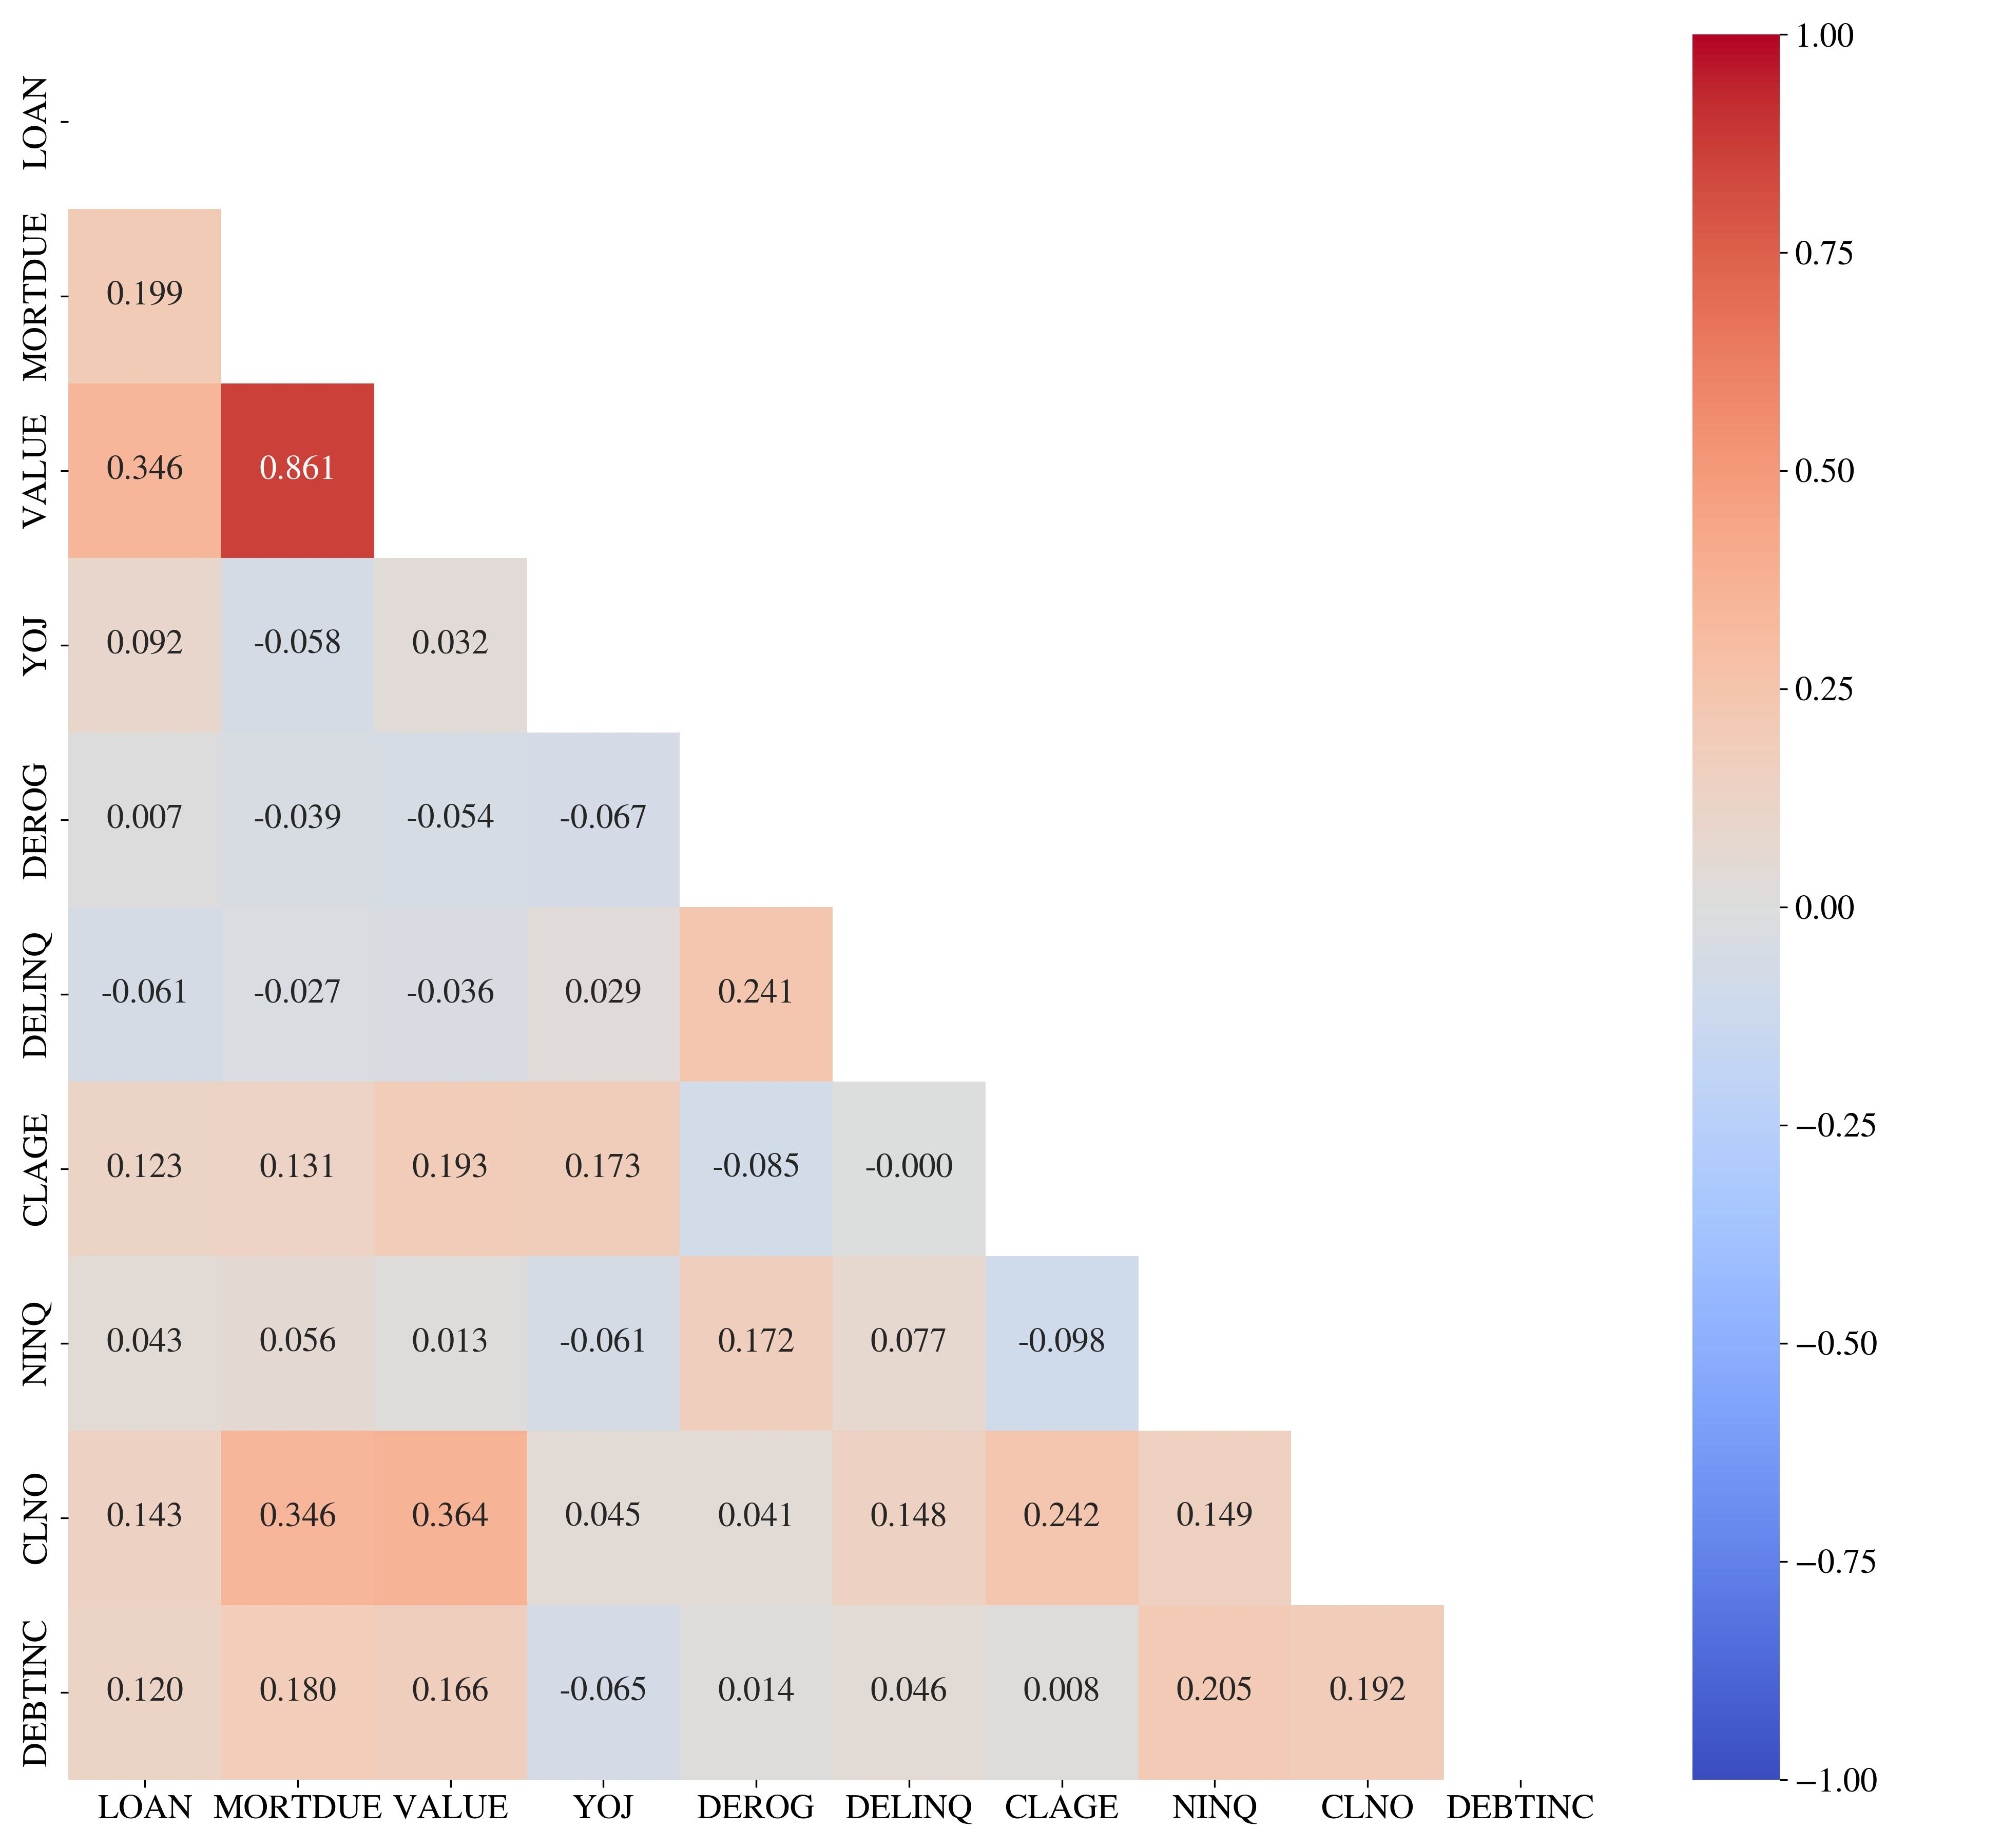
\includegraphics[width=150mm]{Figures/Spearman_Correlation_Matrix_Numeric_Features.jpg}

    \centering{\begin{source}Author's results in Python\end{source}}\vspace{-1em}
\end{figure}

Regarding the association between categorical features, namely \texttt{REASON} and \texttt{JOB}, the Cramer's V coefficient is used. The Cramer's V coefficient results in a value of 0.149 while being statistically significant at 1\% the significance level, thus, we observe a weak association between the two features.


\newpage
\section{Data Preprocessing}
\label{sec:dataprep}
In this section, the process of preprocessing data is described as a crucial step prior to machine learning modelling. Particularly, the process of dividing data for various tasks, ADASYN oversampling due to the imbalanced class issue, discretization of features and Weight--of--Eveidence transformation are further discussed and employed.

\subsection{Data Split and ADASYN Oversampling}
\label{subsec:data-split-ADASYN}

To ensure appropriate model training and unbiased evaluation, it is necessary to split the data into separate sets for various purposes. Specifically, the data set is split into three sets: (1) training set for training the model, feature selection or hyperparameter tuning, (2) validation set for model selection, and (3) test set to assess the model's performance on the unseen data \citep{subasi2020practical}.
In this thesis, the data is split into training, validation, and test sets with a ratio of 70:15:15, which ensures a sufficient amount of data for training, hence the model would be able to generalize well, while keeping the validation and test sets large enough to provide reliable evaluation of the model's performance.


The data is split using stratified splitting to preserve the default status distribution, which is highly imbalanced.
Stratification ensures that the distribution of defaults and non-defaults remains the same across all sets, thereby avoiding overfitting and data leakage. Using stratification, each set had 80 \% non-defaults and 20 \% defaults. This method enables accurate prediction since the model is trained and evaluated on the same population \citep{igareta2021strat}.

However, stratification alone may not be sufficient for dealing with imbalanced classes. Therefore, ADASYN oversampling is performed as described in \autoref{sec:adasyntheory}. Note that ADASYN oversampling is performed on the training set only after the split to avoid data leakage and biased evaluation.


In Python, the data are divided and oversampled using a custom function \lstinline{data_split()}.
This function first employs the \lstinline{train_test_split()} function from the \lstinline{scikit-learn} module to split the data into training, validation, and test sets with a stratification technique.
Next, the \lstinline{ADASYN()} class from the \lstinline{imblearn} module is used to oversample the training set. This is achieved by generating synthetic instances of the minority class based on the five nearest neighbors and Euclidean distance.

However, the \lstinline{ADASYN()} class from \lstinline{imblearn} is not designed to handle missing values or categorical features encoded as character. To overcome this limitation, the following approach is taken:
\begin{enumerate}\setlength\itemsep{0em} 
\item Separate the categorical and numeric features;
\item Impute the missing values with arbitrary values:
\begin{itemize}
\item Categorical features: string \lstinline{'N/A'};
\item Numeric features: number \lstinline{99999999999999} - such value is chosen since it is highly unlikely to be present in the data set.
\end{itemize}
\item Convert the categorical features into dummy variables;
\item Join the numeric features with the dummy variables;
\item Perform the oversampling on the joined data set;
\item Convert the dummy variables back into categorical features;
\item Retrieve back the missing values:
\begin{itemize}
\item Categorical features: replace string \lstinline{'N/A'} with \lstinline{np.nan};
\item Numeric features: for each feature $X$ if its value exceeds its original maximum value, then replace it with \lstinline{np.nan};
\end{itemize}
\end{enumerate}


The following \autoref{tab:split} shows the default distribution of the individual sets before and after oversampling. The default distribution in the training set after ADASYN oversampling is balanced, while the default distribution remains the same across the validation and test sets, which is desirable due to stratification.
\begin{table}[H]
\small
\setlength{\tabcolsep}{8pt}
\renewcommand{\arraystretch}{1.3}
\centering
    \caption[Data Split Summary]{Data Split Summary}\label{tab:split}
    \begin{tabular}{lrrr}
\toprule
\textbf{Set} & \textbf{\# instances} & \textbf{\% defaults} & \textbf{\% non--defaults}\\
\midrule
\hline
Training & 4,171  & 19.95 \% & 80.05 \% \\
Training (oversampled) & 6,437 &  48.13 \% & 51.87 \% \\

Validation & 895 &  20.00 \% & 80.00 \% \\

Test & 894 &  20.00 \% & 80.00 \% \\
\hline
\bottomrule
\end{tabular}
\vspace{0.7em}

\centering{\begin{source}Author's results in Python\end{source}}\vspace{-1em}
\end{table}
\newpage

Since ADASYN increases the sample size by generating, i.e., adding new instances to the sample, it may have an impact on the distribution of the features.
After the inspection in Python, it has no significant impact on the numeric features as the distributions before and after ADASYN oversampling do not differ that much, as can be seen \autoref{fig:adasynimpactnum} in \autoref{chap:app1}.
However, pertaining to the categorical features, a significant impact of ADASYN oversampling can be observed, as can be seen in \autoref{tab:adasynimpact} and \autoref{fig:adasynimpact}, respectively, which depict the distribution of categorical features on the subsample of default cases within the training set, particularly distribution before and after the oversampling.
As such, $n_B$ and $n_A$ refer to the number of default cases within a given category before and after oversampling, respectively, and $N_B$ and $N_A$ represent the total number of default cases before and after oversampling, respectively.


Within the \texttt{REASON} feature, we can observe a significant increase in the proportion of defaulted clients who applied for a loan due to the debt consolidation (\texttt{DebtCon}) among all the defaulters after an oversampling - particularly, the ratio has increased by 12.20 percentage points.
Regarding the \texttt{JOB} feature, we can observe a substantial increase in the proportion of defaulted managers (\texttt{Mgr}) among all the defaulters after oversampling by 38.75 percentage points.
\begin{table}[H]
    \small
    \setlength{\tabcolsep}{8pt}
    \renewcommand{\arraystretch}{1.3}
    \centering
    \caption[ADASYN Impact on Categorical Features' Distribution]{ADASYN Impact on Categorical Features' Distribution}\label{tab:adasynimpact}
    \begin{tabular}{ll|rr|rr|r}
    
        \hline
    \textbf{Features} & \textbf{Category} & \textbf{$n_{B}$} & \textbf{$n_{A}$} & \textbf{$n_{B} / N_{B}$} & \textbf{$n_{A} / N_{A}$} & \textbf{Diff.} \\ 
    \midrule
    \midrule
    REASON & DebtCon & 528 & 2,344 & 63.46 \% & 75.66 \% & 12.20 p.p. \\ 
    REASON & HomeImp & 274 & 720 & 32.93 \% & 23.24 \% & -9.69 p.p. \\
    REASON & N/A & 30 & 34 & 3.61 \% & 1.10 \% & -2.51 p.p. \\
    \hline
    JOB & Mgr & 124 & 1,662 & 14.9 \% & 53.65 \% & 38.75 p.p. \\ 
    JOB & Other & 396 & 943 & 47.6 \% & 30.44 \% & -17.16 p.p. \\ 
    JOB & ProfExe & 142 & 272 & 17.07 \% & 8.78 \% & -8.29 p.p. \\ 
    JOB & Office & 85 & 104 & 10.22 \% & 3.36 \% & -6.86 p.p. \\ 
    JOB & Self & 39 & 58 & 4.69 \% & 1.87 \% & -2.82 p.p. \\
    JOB & Sales & 29 & 36 & 3.49 \% & 1.16 \% & -2.33 p.p. \\ 
    JOB & N/A & 17 & 23 & 2.04 \% & 0.74 \% & -1.30 p.p. \\ 
    \hline
    \bottomrule
    \end{tabular}
    \vspace{0.7em}
    
    \centering{\begin{source}Author's results in Python\end{source}}\vspace{-1em}
\end{table}
\newpage
Such findings regarding the significant increases in the proportion of default cases regarding the \texttt{DebtCon} and \texttt{Mgr} categories are given to the nature of ADASYN oversampling.
As already explained, ADASYN generates more synthetic default class instances in the neighborhood of such default instances, which are hard--to--learn for ADASYN.
In other words, ADASYN creates more default instances for such default instances where the density of the non--default class is relatively high in given default class instance's neighborhood.
Therefore, default instances which either are managers or applied for a loan due to the debt consolidation are difficult--to--learn for ADASYN, thus ADASYN replicates more instances with such characteristics, hence this results in a higher proportion of default cases in the oversampled set for such category.


\begin{figure}[H]
    \centering
    \caption{ADASYN Impact of Categorical Features' Distribution}\vspace{0.5em}
    \label{fig:adasynimpact}\
    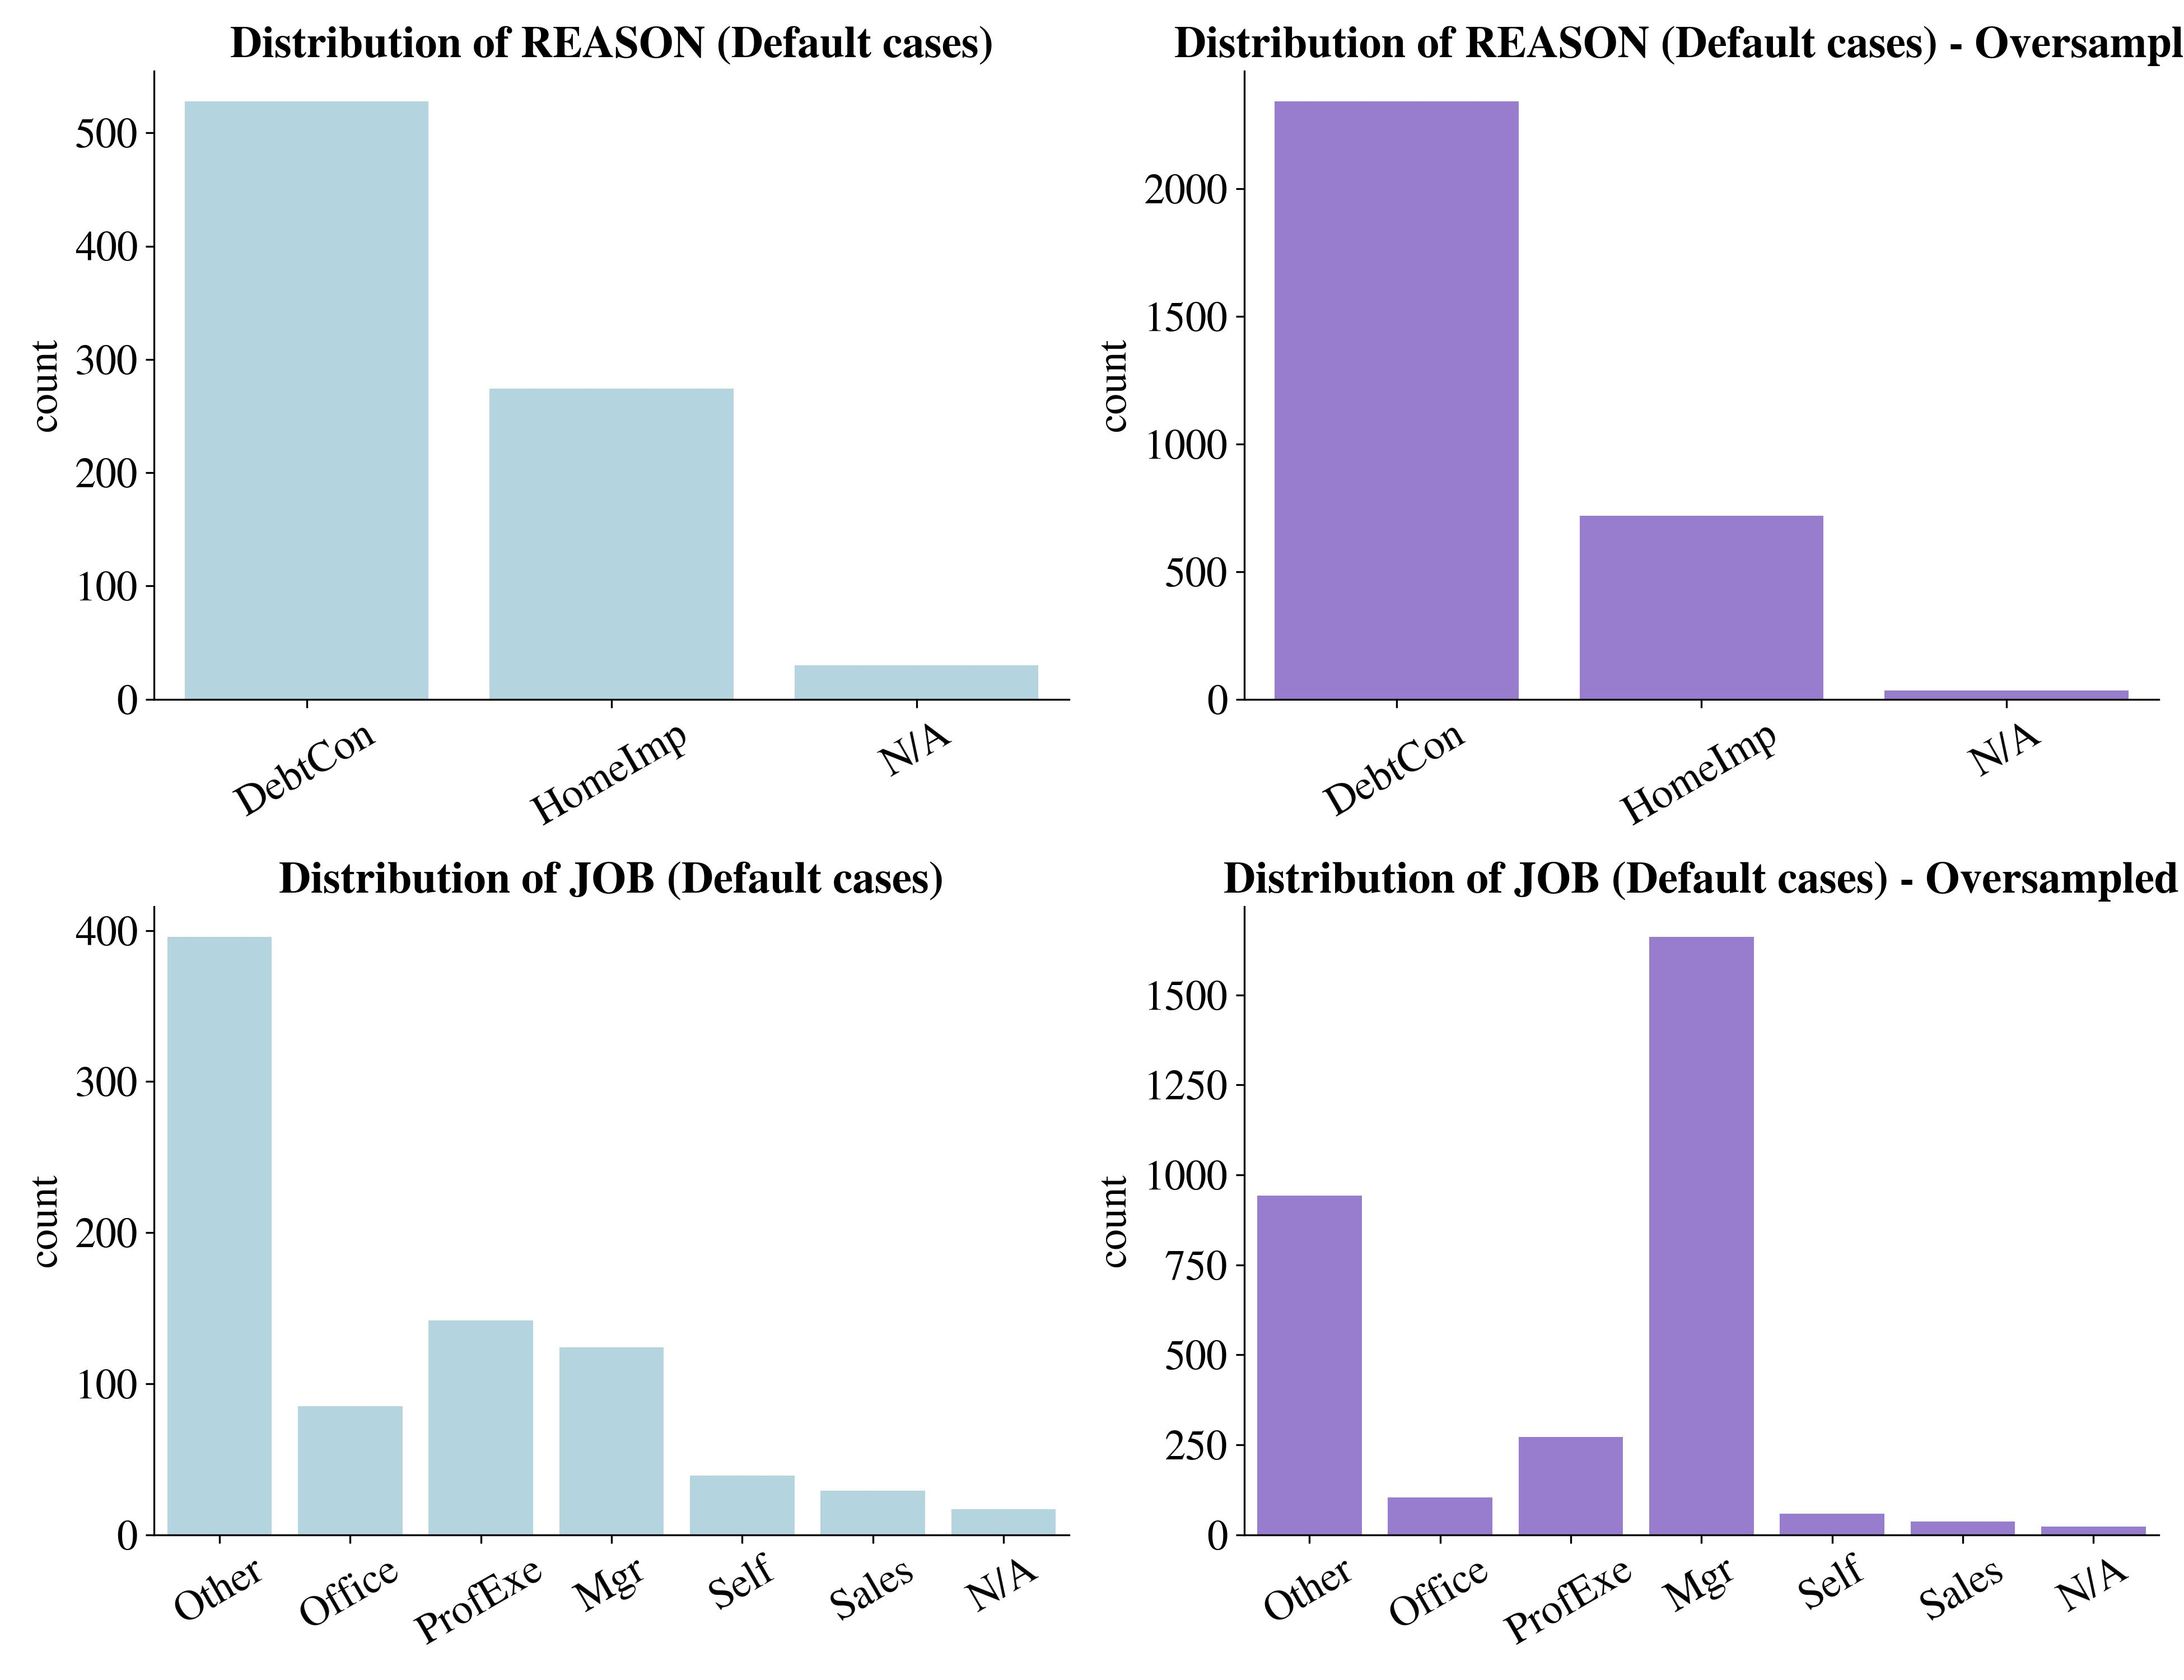
\includegraphics[width=130mm]{Figures/Categorical_Features_Distribution_OS_Default.jpg}

    \centering{\begin{source}Author's results in Python\end{source}}\vspace{-1em}
\end{figure}



\newpage
\subsection{Optimal Binning and Weight--of--Evidence}
\label{subsec:prep-optbinning}
As already described in \autoref{sec:optbinningtheory}, the Optimal Binning is employed as a data preprocessing step in this thesis.
Particularly, we employ \lstinline{BinningProcess} class from the \lstinline{optbinning} module in Python - such class optimally discretizes the continuous features into interval bins and optimally groups categorical features' categories into sub-group categories with respect to the target variable while maximizing Information Value, and afterwards such bins are encoded using WoE \citep{navas2020optimal}. Besides discretizing and grouping, it also creates special bins for capturing missing values.


In this thesis, this data preprocessing step is wrapped into a custom function \lstinline{woe_binning()} in Python.
First, the \lstinline{BinningProcess} class is fitted on the training set only in order to avoid data leakage, while it learns the split points for binning, event rates, WoE coefficients, etc., and then is used to transform the training, validation, and test set.


The following \autoref{fig:woedistdebtinc} depicts the WoE bins distribution for the \texttt{DEBTINC} feature.
It is evident that the bin capturing the missing values has the most negative WoE coefficient, which indicates a larger distribution of defaulters compared to non--defautlters in such bin. We can further observe a monotonic relationship between the WoE coefficients and the bins, as the debt--to--income ratio increases, the WoE coefficient decreases, thus higher likelihood of default.
Therefore, we expect that if the debt--to--income ratio is either missing or extremely high, it will have a significant impact on the likelihood of default.
\begin{figure}[H]
    \centering
    \caption{WoE Bins Distribution - Debt--To--Income Ratio}\vspace{0.5em}
    \label{fig:woedistdebtinc}
    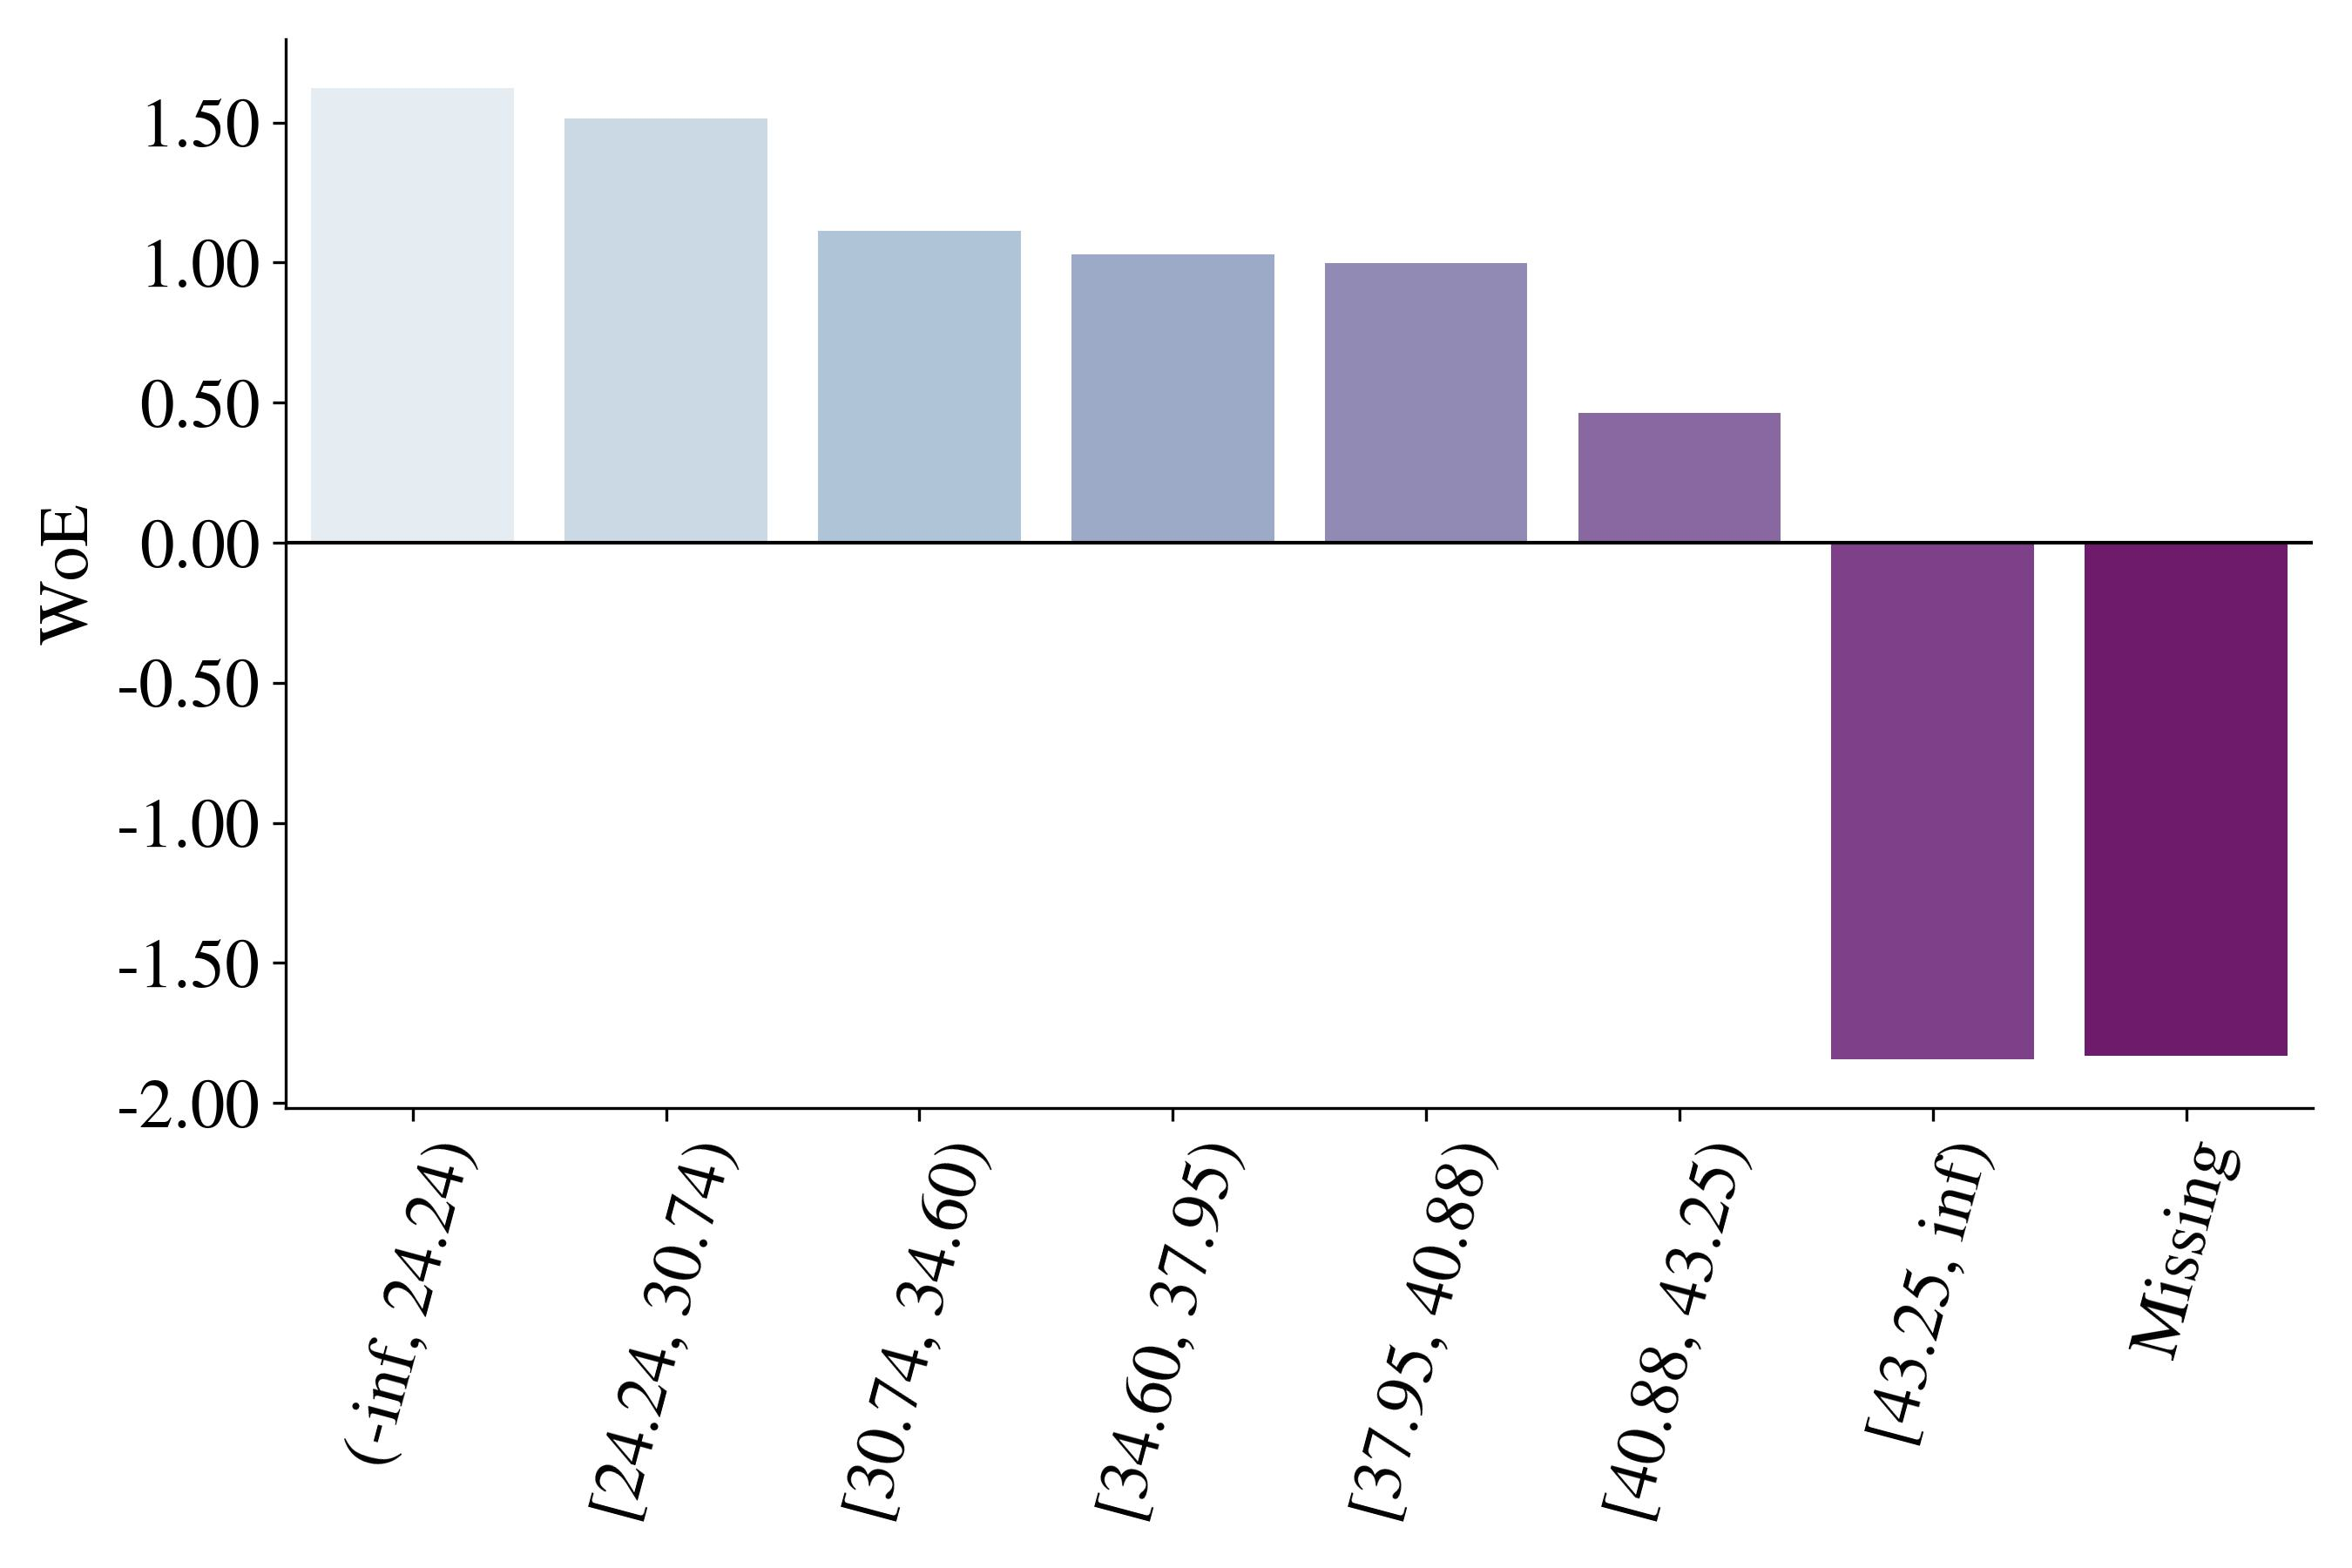
\includegraphics[width=120mm]{Figures/WoE_Distribution_DEBTINC.jpg}
    
    \centering{\begin{source}Author's results in Python\end{source}}\vspace{-1em}
\end{figure}

Another monotonic relationship can be observed in case of \texttt{DELINQ} feature as can be seen in \autoref{fig:woedistdelinq}. With increasing number of delinquent credit lines, the WoE coefficient decreases, indicating a larger distribution of defaulters compared to non--defaulters. Therefore, we expect that the higher the number of delinquent credit lines will lead to the higher the likelihood of default.


\begin{figure}[H]
    \centering
    \caption{WoE Bins Distribution - Number of Delinquent Credit Lines}\vspace{0.5em}
    \label{fig:woedistdelinq}
    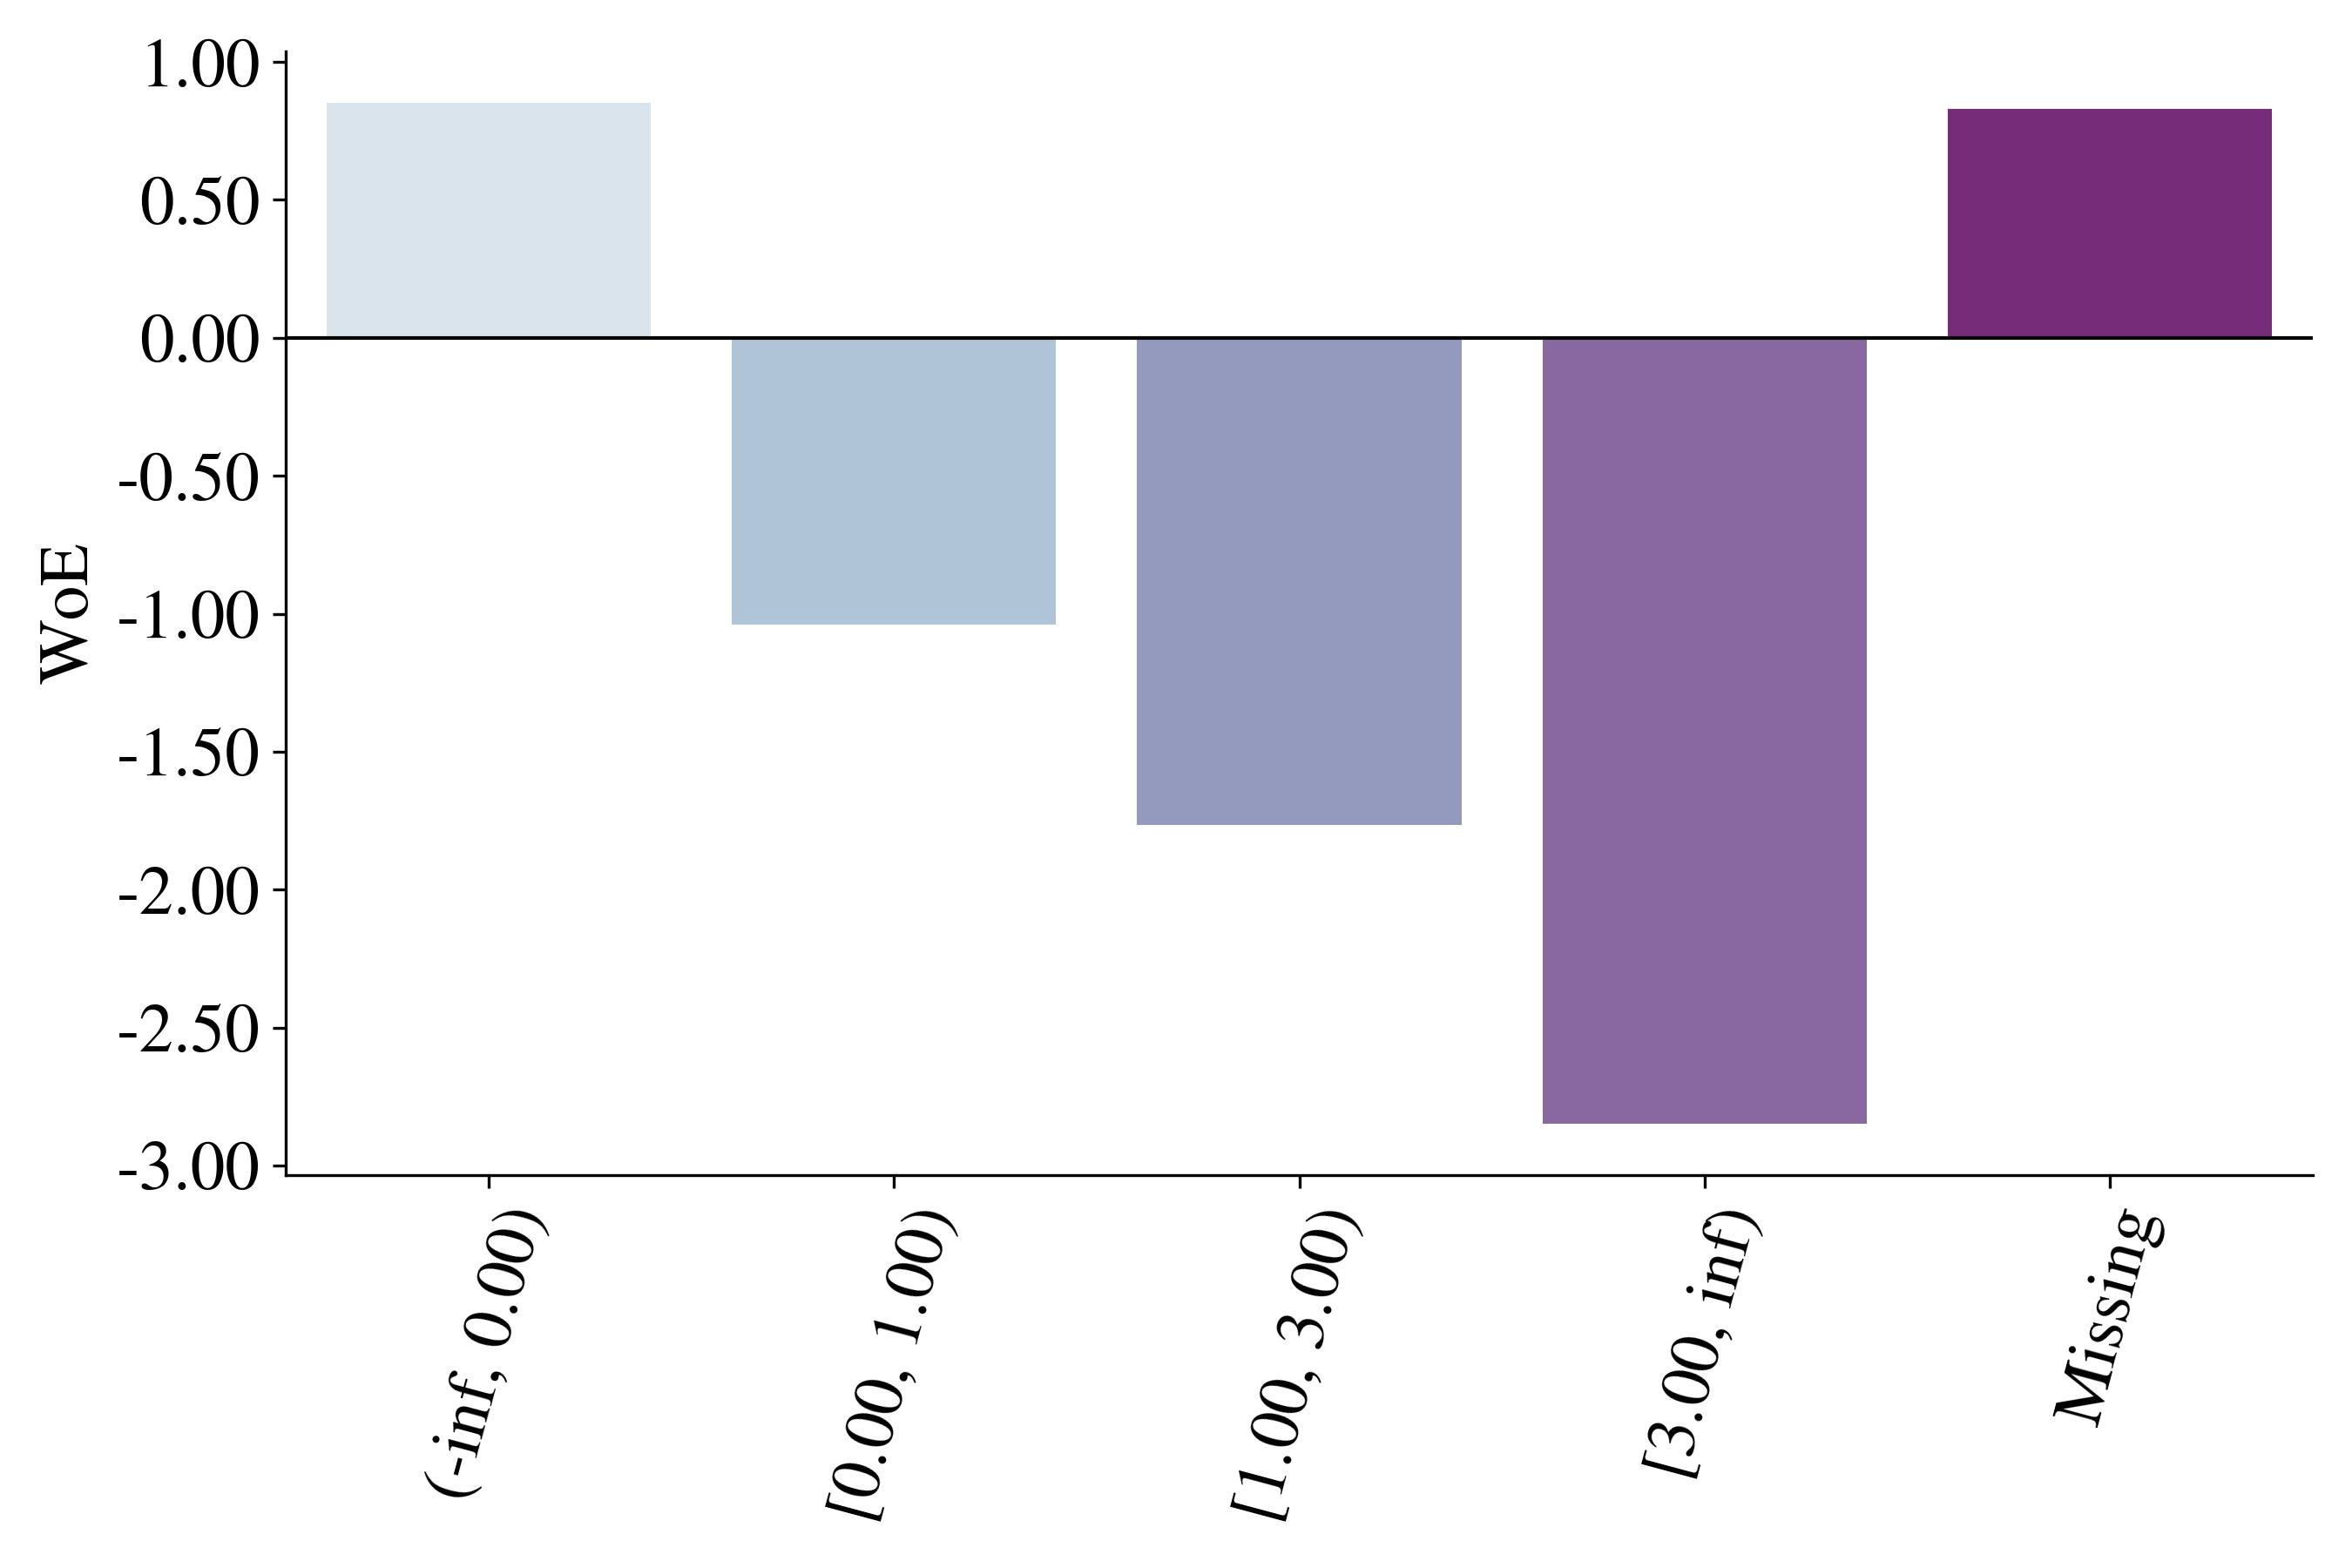
\includegraphics[width=120mm]{Figures/WoE_Distribution_DELINQ.jpg}
    
    \centering{\begin{source}Author's results in Python\end{source}}\vspace{-1em}
\end{figure}

Within the \texttt{JOB} feature, specifically regarding the \texttt{Mgr} category, we can observe in \autoref{fig:woedistjob} the direct impact of ADASYN oversampling as already described by \autoref{tab:adasynimpact}.
Since ADASYN generated more default class instances for original default instances who are managers, this results in a higher default rate within such job category, leading to a larger distribution of defaulters compared to non--defaulters, which is quantified in the negative WoE value.
We can also see, that Optimal Binning has grouped categories \texttt{Self}, \texttt{Sales} and \texttt{Others} into a single category bin.



\begin{figure}[H]
    \centering
    \caption{WoE Bins Distribution - Job Occupancy}\vspace{0.5em}
    \label{fig:woedistjob}
    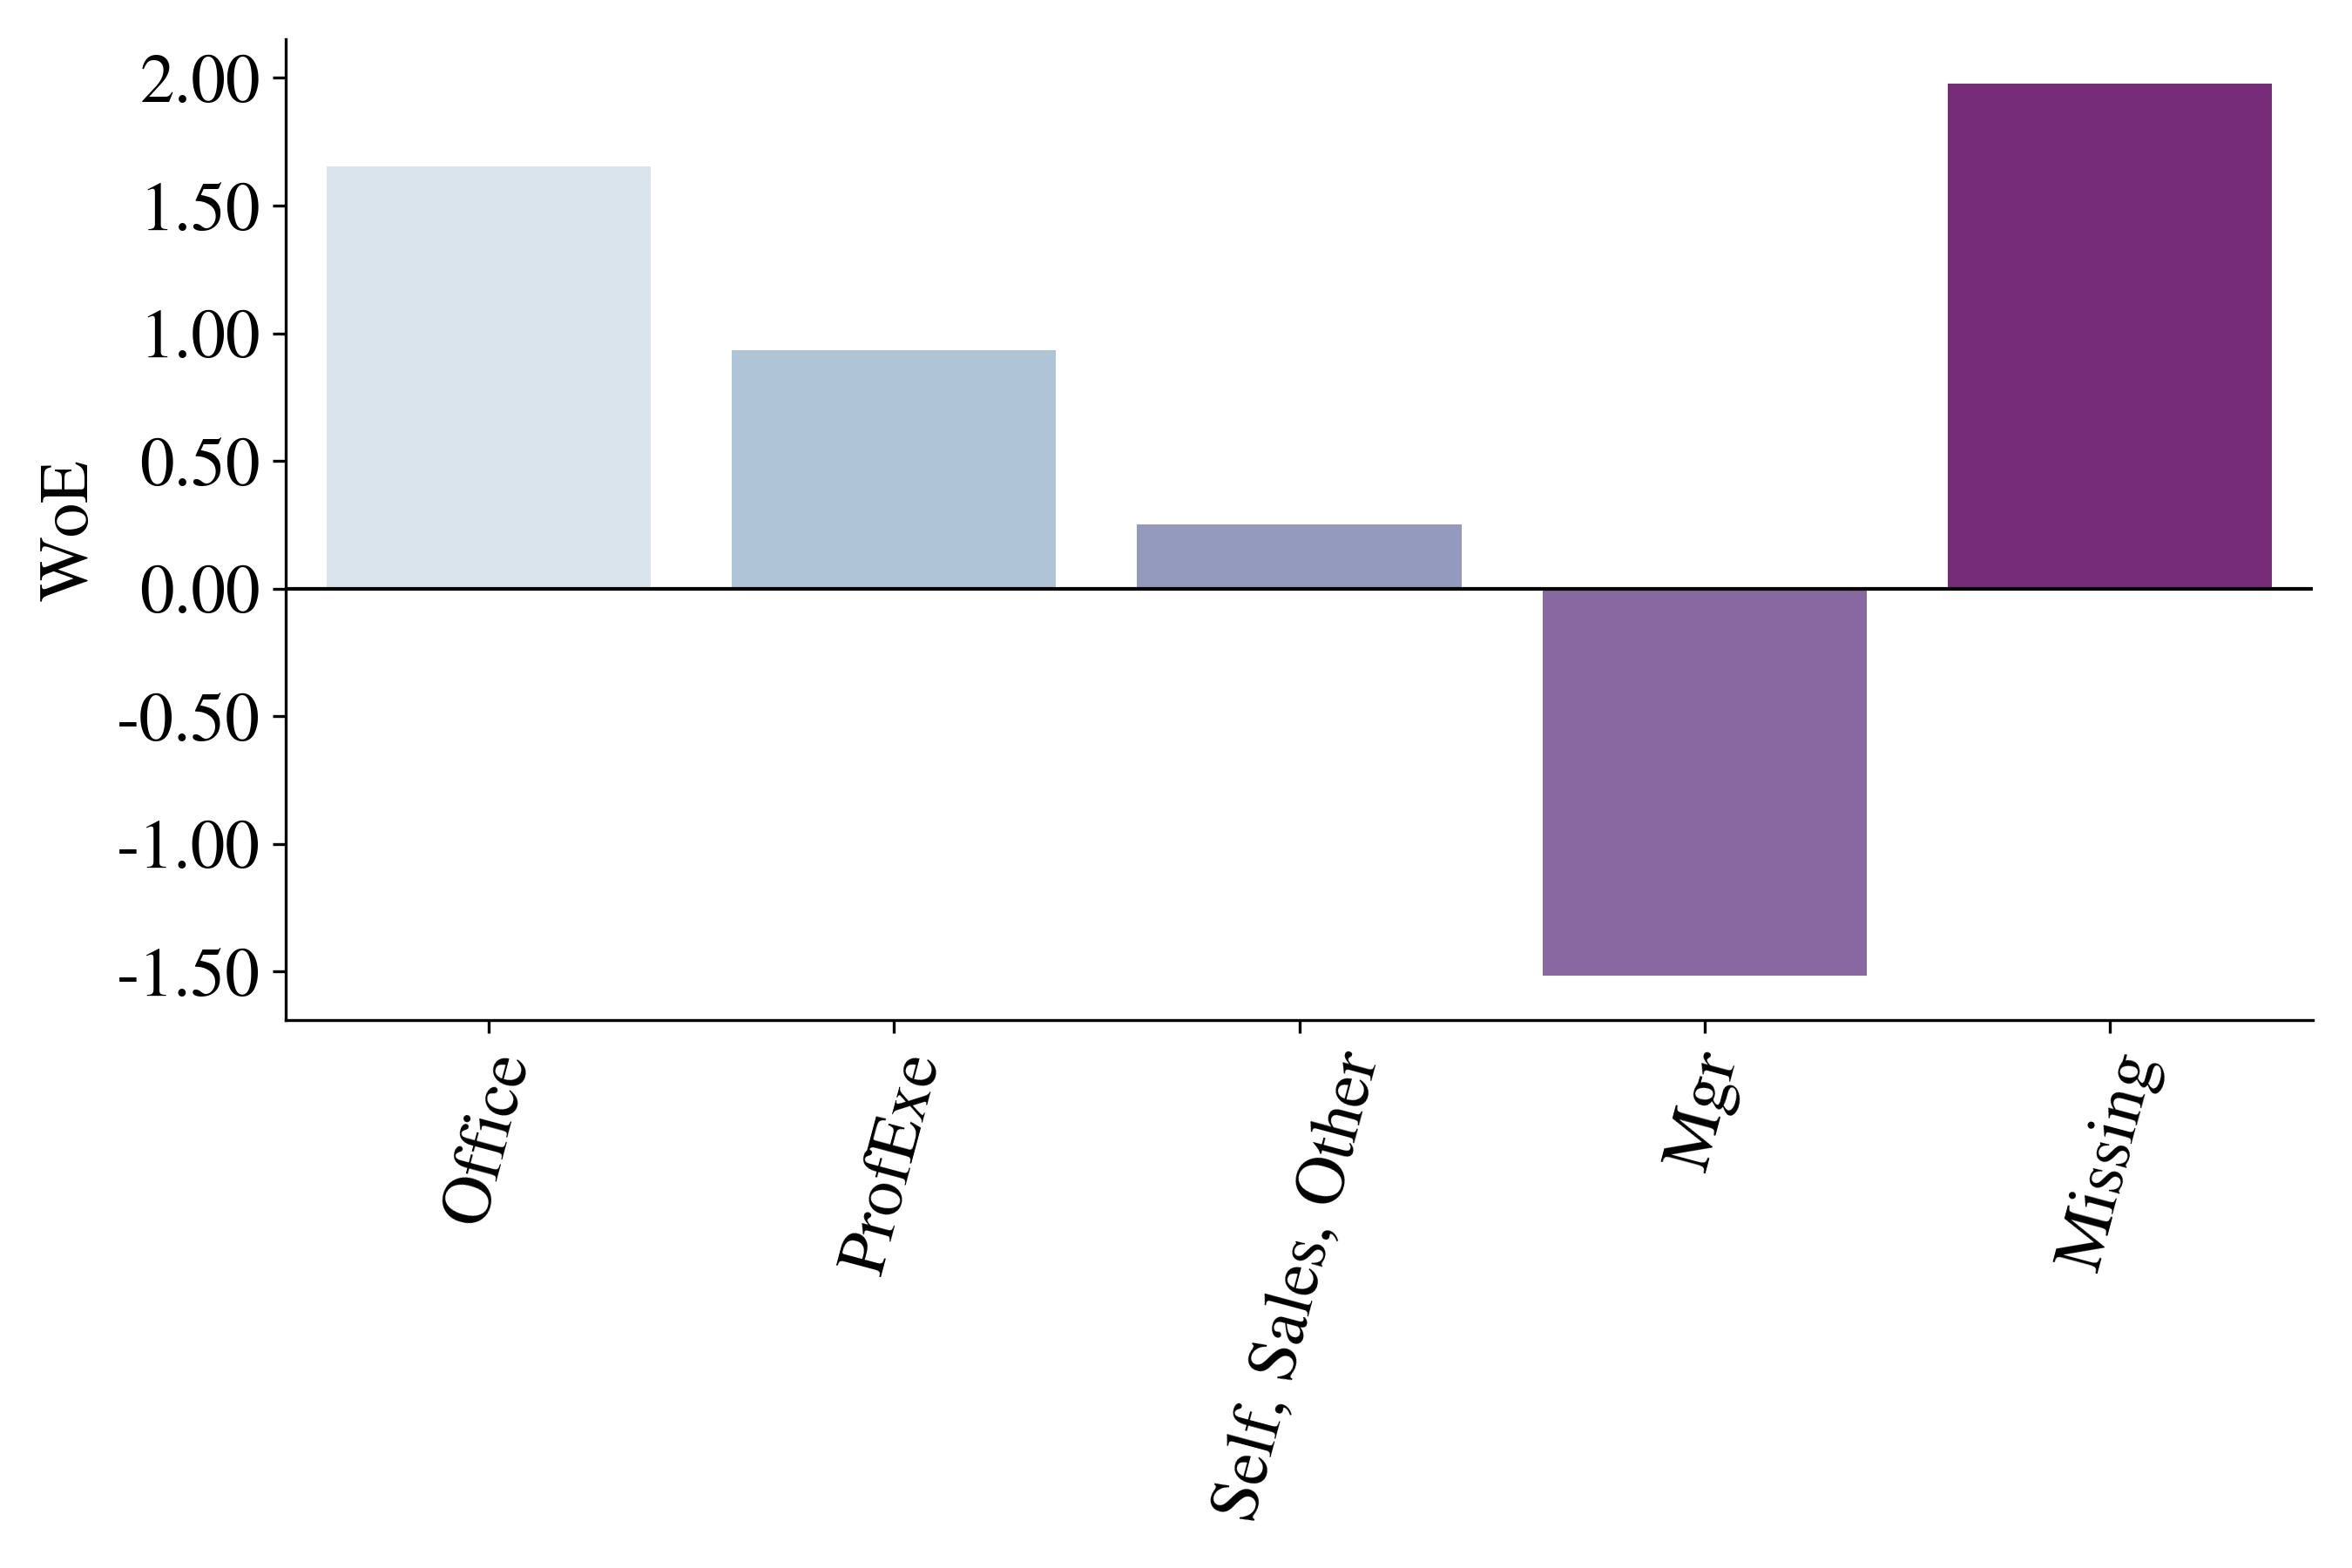
\includegraphics[width=120mm]{Figures/WoE_Distribution_JOB.jpg}
    
    \centering{\begin{source}Author's results in Python\end{source}}\vspace{-1em}
\end{figure}

The WoE bins distributions of other features are depicted \autoref{fig:woedist} in the Appendix \autoref{chap:app1}.



\newpage
\section{Modelling}
\label{sec:modelling}
Once the data are finally preprocessed, the next step regards the modelling part which includes hyperparameter tuning, feature selection, model selection, and model recalibration.
In Python, eight different machine learning classification models from \lstinline{Scikit-learn} module are used for the default status prediction, which were already described in \autoref{sec:algorithms}, namely:
\begin{itemize}\setlength\itemsep{0em}
\item \textbf{Logistic Regression} - \lstinline{LogisticRegression()}
\item \textbf{Decision Tree} - \lstinline{DecisionTreeClassifier()}
\item \textbf{Gaussian Naive Bayes} - \lstinline{GaussianNB()}
\item \textbf{K-Nearest Neighbors} - \lstinline{KNeighborsClassifier()}
\item \textbf{Random Forest} - \lstinline{RandomForestClassifier()}
\item \textbf{Gradient Boosting} - \lstinline{GradientBoostingClassifier()}
\item \textbf{Support Vector Machine} - \lstinline{SVC()}
\item \textbf{Multi--Layer Perceptron} (\textit{Neural Network}) - \lstinline{MLPClassifier()}
\begin{itemize}\setlength\itemsep{0em}
\item Henceforth, terms such as Neural Network and Multi--Layer Perceptron are used interchangeably.
\end{itemize}
\end{itemize}

\subsection{Bayesian Hyperparameter Optimization}
\label{subsec:hyperoptbayes}
In this thesis, hyperparameter tuning of models is performed using Bayesian Optimization as described in \autoref{sec:bayesoptheory}.
In Python, a custom function, \lstinline{bayesian_optimization()}, is implemented to perform hyperparameter tuning using Bayesian Optimization.
This function utilizes \lstinline{BayesSearchCV} class from the \lstinline{Scikit-optimize} module, with a 10-fold stratified cross-validation scheme and 50 iterations, while maximizing the F1 score. As a surrogate function, the Gaussian Process is used \citep{scikit-opt}.
The use of \lstinline{BayesSearchCV} with stratified cross-validation in the hyperparameter tuning process provides a robust and reliable approach to selecting the optimal hyperparameters for the model, while the incorporation of Bayesian Optimization enables the efficient exploration of the hyperparameter space.
By maximizing the F1 score, the hyperparameters selected through this process will result in a model with improved performance. Note, that the hyperparameter tuning is performed solely on training set in order to preserve the independence of the validation and test set, and avoid information and data leakage as well.

For each model, the Bayesian Optimization algorithm performs 50 iterations while searching for the best hyperparameters values that maximize the F1 score. Within each iteration, a 10-fold stratified cross-validation is conducted to evaluate the model's cross--validation F1 score.
Moreover, for each model, we specify the hyperparameter space, i.e., the particular hyperparameters to be tuned and their possible ranges that the hyperparameter can take. The ranges are specified using \lstinline{Integer} class to define an interval of integers, \lstinline{Real} to define an interval of float numbers, and \lstinline{Categorical} to define a list of possible (categorical) values.
Note that not all the available hyperparameters are tuned, but only the most relevant ones due to the time complexity of the Bayesian Optimization algorithm.
The definition of hyperparameter space for each model is described further in the following subsubsections.

\subsubsection{Logistic Regression}
The first hyperparameter \textbf{\texttt{Intercept}} allows us to specify whether the intercept should be estimated or not.
$C$ is the regularization strength, and it is used to specify the regularization factor, which is further specified with the hyperparameter \textbf{\texttt{Penalty}}.
If the penalty is set to $ElasticNet$, we can also tune $L1$ ratio, which refers to the $\alpha$ parameter in in \autoref{eq:elasticnet}
Moreover, the \textbf{\texttt{Class weight}} hyperparameter is a hyperparameter that allows us to assign higher importance to minority class instances during the training process.


\textbf{\texttt{Solver}} hyperparameter is used to specify which optimization algorithm should be used to estimate the parameters.
According to Hale \citep{hale2019dont}, Scikit-learn provides five solvers for Logistic Regression, namely \textit{lbfgs} (Limited-memory Broyden-Fletcher-Goldfarb-Shanno) which approximates the second derivative matrix updates with gradient evaluations, \textit{liblinear} (Library for Large Linear Classification) which uses the coordinate descent algorithm, \textit{newton-cg},
\textit{sag} (Stochastic Average Gradient descent) as a variation of gradient descent and incremental aggregated gradient approaches using a random sample of previous gradient values, and \textit{saga} as an extension of \textit{sag} which allows $L1$ regularization.
For more information, please refer to the Scikit-learn documentation \citep{scikit-lr}.
The last hyperparameter of Logistic Regression to tune in this thesis is the \textbf{\texttt{Intercept scaling}} which allows to scale the intercept.

\begin{table}[H]
\small
\setlength{\tabcolsep}{8pt}
\renewcommand{\arraystretch}{1.3}
\centering
    \caption[Logistic Regression - Hyperparameter Space]{Logistic Regression - Hyperparameter Space}\label{tab:lrspace}
    \begin{tabular}{ll}
\toprule
\textbf{Hyperparameter} & \textbf{Space}\\
\midrule
\hline
Intercept & True, False \\
$C$ factor & <$1\times10^{-6}$, 5>\\
Penalty & L1, L2, Elastic Net, None \\
Solver & lbfgs, liblinear, newton-cg, sag, saga \\
Class weight & None, balanced \\
L1 ratio & <0, 1> \\
Intercept scaling & True, False  \\
\hline
\bottomrule
\end{tabular}
\vspace{0.7em}

\centering{\begin{source}Author's results in Python\end{source}}\vspace{-1em}
\end{table}


\subsubsection{Decision Tree}
The first hyperparameter of Decision Tree is the \textbf{\texttt{Criterion}} which allows us to specify the function to measure the quality of a split - either Gini or Entropy impurity function.
Another important hyperparameter is the \textbf{\texttt{Max depth}} which allows us to specify the maximum depth of the tree.
The last hyperparameter is the \textbf{\texttt{Max features}} which allows to specify the number of features to consider when looking for the best split \citep{scikit-dt}.
Note, that \textbf{\texttt{Max features}} has a variable range of values depending on the number of features, which is dependent on the number of features selected during feature selection (where the features are iteratively selected and the model is trained and evaluated on each iteration).
\begin{table}[H]
\small
\setlength{\tabcolsep}{8pt}
\renewcommand{\arraystretch}{1.3}
\centering
    \caption[Decision Tree - Hyperparameter Space]{Decision Tree - Hyperparameter Space}\label{tab:dtspace}
    \begin{tabular}{ll}
\toprule
\textbf{Hyperparameter} & \textbf{Space}\\
\midrule
\hline
Criterion & Gini, Entropy \\
Max depth & <1, 10> \\
Max features & <1, \verb|len(X.columns)|>  \\
\hline
\bottomrule
\end{tabular}
\vspace{0.7em}

\centering{\begin{source}Author's results in Python\end{source}}\vspace{-1em}
\end{table}

\newpage
\subsubsection{Gaussian Naive Bayes}

In the case of Gaussian Naive Bayes, the only hyperparameter to tune is the \textbf{\texttt{Variance smoothing}} which allows to specify the portion of the largest variance of all features to be added to variances for calculation stability \citep{scikit-gnb}, in order to smooth out the variances of each feature in case when the variance is zero.
\begin{table}[H]
\small
\setlength{\tabcolsep}{8pt}
\renewcommand{\arraystretch}{1.3}
\centering
    \caption[Gaussian Naive Bayes - Hyperparameter Space]{Gaussian Naive Bayes  - Hyperparameter Space}\label{tab:gnbspace}
    \begin{tabular}{ll}
\toprule
\textbf{Hyperparameter} & \textbf{Space}\\
\midrule
\hline
Variance smoothing & <$1\times 10^{-9}$, $1\times 10^{-6}$> \\
\hline
\bottomrule
\end{tabular}
\vspace{0.7em}

\centering{\begin{source}Author's results in Python\end{source}}\vspace{-1em}
\end{table}


\subsubsection{K--Nearest Neighbors}

In KNN, it is crucial to specify the number of neighbors to consider during the classification process, which is depicted in the \textbf{\texttt{\# neighbors}} hyperparameter.
Further, it is needed to select the optimal distance measure, i.e., Euclidean, Manhattan, or Minkowski, as described in \autoref{subsec:knn-theory} - such selection refers to the \textbf{\texttt{Metric}} hyperparameter.
Pertaining to the Minowski distance, we also tune the \textbf{\texttt{Norm order}} hyperparameter which allows us to specify the power parameter within the distance calculation.
Last but not least, KNN also allows us to tune the \textbf{\texttt{Weights}} hyperparameter which allows us to specify the weight function used in prediction - either uniform or distance. With the former function, all the points within each neighborhood are weighted uniformly, and with the latter approach, the points are weighted inversely with respect to their distance. \citep{scikit-knn}.
\begin{table}[H]
\small
\setlength{\tabcolsep}{8pt}
\renewcommand{\arraystretch}{1.3}
\centering
    \caption[K--Nearest Neighbors - Hyperparameter Space]{K--Nearest Neighbors - Hyperparameter Space}\label{tab:knnspace}
    \begin{tabular}{ll}
\toprule
\textbf{Hyperparameter} & \textbf{Space}\\
\midrule
\hline
\# neighbors & <5, 20> \\
Metric & Euclidean, Manhattan, Minkowski \\
Norm order & <1, 5> \\
Weights & Uniform, Distance \\
\hline
\bottomrule
\end{tabular}
\vspace{0.7em}

\centering{\begin{source}Author's results in Python\end{source}}\vspace{-1em}
\end{table}

\subsubsection{Random Forest}
In the Random Forest, we tune the number of base trees that are trained in parallel way in the ensemble, i.e., the \textbf{\texttt{\# estimators}} hyperparameter.
Similarly to Decision Tree, Random Forest allows to select the optimal split measure, i.e., Gini, Entropy or additionally even Log Loss, which is depicted in the \textbf{\texttt{Criterion}} hyperparameter.
Likewise Decision Tree, Random Forest also allows us to specify the maximum depth of the tree as well as the number of features to consider when looking for the best split, i.e., the \textbf{\texttt{Max depth}} hyperparameter and \textbf{\texttt{Max features}}, respectively.
The \textbf{\texttt{Bootstrap}} hyperparameter allows us to specify whether bootstrap samples are used when training the tree estimators.

Similarly to Logistic Regression, Random Forest also has the \textbf{\texttt{Class weight}} hyperparameter which allows to specify the weight of each class in the classification process - \textit{balanced} function takes the target variable to adjust the weights, which are inversely proportional to class frequencies, whereas \textit{subsample balanced} does almost the same, but the weights are computed based on the bootstrap samples.
Last but not least, Random Forest also allows to tune the \textbf{\texttt{CCP alpha}} hyperparameter which allows to specify the complexity parameter used for Minimal Cost-Complexity Pruning (CCP), in order to reduce the size of the tree estimators and avoid overfitting by removing subtrees from the tree estimators that do not improve the performance \citep{scikit-rf}.

\begin{table}[H]
\small
\setlength{\tabcolsep}{8pt}
\renewcommand{\arraystretch}{1.3}
\centering
    \caption[Random Forest - Hyperparameter Space]{Random Forest - Hyperparameter Space}\label{tab:rfspace}
    \begin{tabular}{ll}
\toprule
\textbf{Hyperparameter} & \textbf{Space}\\
\midrule
\hline
\# estimators & <100, 1000> \\
Criterion & Gini, Entropy, Log Loss \\
Max depth & <1, 10> \\
Max features & <1, \verb|len(X.columns)|>  \\
Bootstrap & True, False \\
Class weight & None, balanced, subsample balanced \\
CCP alpha & <$1\times10^{-12}$, 0.5> \\
\hline
\bottomrule
\end{tabular}
\vspace{0.7em}

\centering{\begin{source}Author's results in Python\end{source}}\vspace{-1em}
\end{table}

\newpage
\subsubsection{Gradient Boosting}
Likewise Random Forest, Gradient Boosting also allows us to tune the number of base trees that are trained in a sequential way in the ensemble, i.e., the \textbf{\texttt{\# estimators}} hyperparameter, as well as the maximum depth of the tree and the number of features to consider when looking for the best split, i.e., the \textbf{\texttt{Max depth}} hyperparameter and \textbf{\texttt{Max features}}, respectively.
Is it also necessary to tune the \textbf{\texttt{Learning rate}} hyperparameter which shrinks the contribution of each tree, in order to prevent overfitting.
We can also select the optimal loss function of Gradient Boosting (\textbf{\texttt{Loss}} hyperparameter), either Log Loss or Exponential loss function - in the latter case, the model is equivalent to the AdaBoost algorithm \citep{scikit-gb}.
Moreover, the \textbf{\texttt{Criterion}} hyperparameter allows to specify the measurement method of the split quality, i.e., MSE or Friedman MSE, which improves the MSE with Friedman scores \citep{scikit-gb}.

\begin{table}[H]
\small
\setlength{\tabcolsep}{8pt}
\renewcommand{\arraystretch}{1.3}
\centering
    \caption[Gradient Boosting - Hyperparameter Space]{Gradient Boosting - Hyperparameter Space}\label{tab:gbspace}
    \begin{tabular}{ll}
\toprule
\textbf{Hyperparameter} & \textbf{Space}\\
\midrule
\hline
\# estimators & <100, 1000> \\
Max depth & <1, 10> \\
Max features & <1, \verb|len(X.columns)|>  \\
Learning rate & <0.0001, 0.2> \\
Loss & Log Loss, Exponential \\
Criterion & MSE, Friedman MSE \\
\hline
\bottomrule
\end{tabular}
\vspace{0.7em}

\centering{\begin{source}Author's results in Python\end{source}}\vspace{-1em}
\end{table}

\subsubsection{Support Vector Machine}
Likewise Logistic Regression, SVM also allows us to tune the \textbf{\texttt{C}} hyperparameter for the regularization, as well as the \textbf{\texttt{Kernel}} hyperparameter which specifies the kernel type to be used in the algorithm in to map the data into higher dimensional space in order to find the optimal hyperplane that separates the classes.
If the kernel is $d$-degree polynomial, we can also tune the \textbf{\texttt{Degree}} hyperparameter, which specifies the degree of the polynomial kernel function.
SVM also has the \textbf{\texttt{Class weight}} hyperparameter, which assigns the weights to the input data based on the class frequencies in order to balance the classes.



\begin{table}[H]
\small
\setlength{\tabcolsep}{8pt}
\renewcommand{\arraystretch}{1.3}
\centering
    \caption[Support Vector Machine - Hyperparameter Space]{Support Vector Machine - Hyperparameter Space}\label{tab:svmspace}
    \begin{tabular}{ll}
\toprule
\textbf{Hyperparameter} & \textbf{Space}\\
\midrule
\hline
C factor & <$1\times 10^{-6}$, 5> \\
Kernel & Linear, Poly, RBF, Sigmoid \\
Degree & <1, 10> \\
Class weight & balanced, None \\
\hline
\bottomrule
\end{tabular}
\vspace{0.7em}

\centering{\begin{source}Author's results in Python\end{source}}\vspace{-1em}
\end{table}


\subsubsection{Multi--Layer Perceptron}
Regarding the MLP, we use one hidden layer where we tune the number of units as represented by the \textbf{\texttt{Hidden layer size}} hyperparameter.
We also tune the \textbf{\texttt{Activation function}} applied in the hidden layer, namely Logistic, ReLU, and Tanh, which were already described in \autoref{subssec:nn}, and further Identity, which is just a linear activation function, hence $f(z) = z$.
Regarding the optimization algorithm, which refers to \textbf{\texttt{Solver}} hyperparameter, we can choose between \textit{lbgfs}, \textit{sgd} (Stochastic Gradient Descent), and \textit{adam} (Adaptive Moment Estimation).
The \textbf{\texttt{Learning rate}} can be either constant (i.e., 0.001), inversely scaled, i.e., gradually and inversely decreased with an inverse scaling exponent $t$ (where $t$ refers to the time step, by default $t=0.5$), or adaptive, i.e., the learning rate is kept constant as long as the training loss keeps decreasing, otherwise it is divided by 5 \citep{scikit-mlp}.

\begin{table}[H]
\small
\setlength{\tabcolsep}{8pt}
\renewcommand{\arraystretch}{1.3}
\centering
    \caption[Multi Layer Perceptron - Hyperparameter Space]{Multi Layer Perceptron - Hyperparameter Space}\label{tab:mlpspace}
    \begin{tabular}{ll}
\toprule
\textbf{Hyperparameter} & \textbf{Space}\\
\midrule
\hline
Hidden layer size & <5, 500> \\
Activation function & Identity, Logistic, Tanh, ReLU \\
Solver & Adam, sgd, lbfgs \\
Learning rate & Constant, Adaptive, Invscaling \\
\hline
\bottomrule
\end{tabular}
\vspace{0.7em}

\centering{\begin{source}Author's results in Python\end{source}}\vspace{-1em}
\end{table}

\newpage
\subsection{Sequential Feature Selection}
\label{subsec:feature-selection}

As the feature selection approach, Forward Sequential Feature Selection (henceforth SFS) is employed in order to choose the optimal set of features as described in \autoref{sec:fsfstheory}.
Within machine learning implementation, instead of fitting Forward SFS only with one model, Forward SFS is fitted to each input model in order to obtain the best subset of features for each model, assuming the importance of each features varies across the models.
Instead of using input models with default hyperparameters, each model is tuned with Bayesian Optimization in order to obtain the optimal hyperparameters for each model, which would further improve the performance of each model within SFS and therefore, it would lead to the more optimal selection of features.
The custom feature selection algorithm is stated in Algorithm \autoref{alg:feature_selection}, thus, when having $n$ input models, it returns $n$ subsets of optimal features, one per each model:
\begin{algorithm}[H]
\caption{Feature Selection Algorithm}
\label{alg:feature_selection}
\begin{algorithmic}[1]
\For{$model \in \textit{models}$}
    \State $\textit{optimized\_model} \gets \textsc{BayesianOptimization}(model)$
    \State $\textit{best\_features} \gets \textsc{ForwardSFS}(\textit{optimized\_model})$
\EndFor
\end{algorithmic}
\end{algorithm}
Particularly, each input model is first tuned on the training set with Bayesian Optimization with 50 iterations and 10--fold stratified cross validation (in order to preserve the target variable distribution across the folds) while maximizing the F1 score - the author's machine learning implementation, his custom function \lstinline{bayesian_optimization()} is used.
Once the model is tuned, the Forward SFS is fitted with such tuned model on the same training set with 10--fold stratified cross validation while maximizing the F1 score. Instead of selecting the fixed number of features, Scikit-learn's \lstinline{SequentialFeatureSelector} class allows to set a stop criterion (\lstinline{tol} parameter) which stops adding features if the objective score function is not increasing at least by \lstinline{tol} between two consecutive feature additions \citep{sfs}.
Such parameter is set to a value that is close to zero, therefore, the feature selection stops when the objective score function is not increasing anymore.

\newpage

Such feature selection algorithm is wrapped into author's custom function \lstinline{SFS_feature_selection()}.
This function iteratively prints the process of the feature selection as can be seen in \autoref{fig:featselectprint}, including the current step (Bayesian Optimization or Feature Selection), the execution time in minutes, and the selected features per each model. Since we have 8 input models, we get 8 optimal subsets of features.

\begin{figure}[H]
\centering\caption{Feature Selection Print Statement}
\label{fig:featselectprint}

{\fontsize{8.8}{11}\selectfont 
\begin{verbatim}
-------------------------------------------------------------------------------------
------------------------------------------ 2/8 --------------------------------------
-------------------------------------------------------------------------------------
------------------------------- FEATURE SELECTION WITH DT ---------------------------
-------------------------------------------------------------------------------------
------------------------------------------------------------------------------------- 

1/4 ... Starting Bayesian Optimization on the whole set of features
2/4 ... Bayesian Optimization finished
3/4 ... Starting Forward Sequential Feature Selection
4/4 ... Forward Sequential Feature Selection with finished 

Execution time: 0.8622 minutes 

9 features selected: VALUE, JOB, YOJ, DEROG, DELINQ, CLAGE, NINQ, CLNO, DEBTINC 

-------------------------------------------------------------------------------------
-------------------------------------------------------------------------------------
\end{verbatim}
}
\centering{\begin{source}Author's results in Python\end{source}}\vspace{0em}
\end{figure}


The following \autoref{fig:fsrec} depicts the recurrence of the selected features. As can be seen, features such as \texttt{CLAGE}, \texttt{DEBTINC}, \texttt{DELINQ} and \texttt{JOB} were selected by each model.
On the other hand, features such as \texttt{LOAN} and \texttt{REASON} were selected only four times. Therefore, it can be expected that such features, which were selected every time, will have a significant impact on predictions.
\begin{figure}[H]
\centering
\caption{Reccurrence of Selected Features}\vspace{0.5em}
\label{fig:fsrec}\
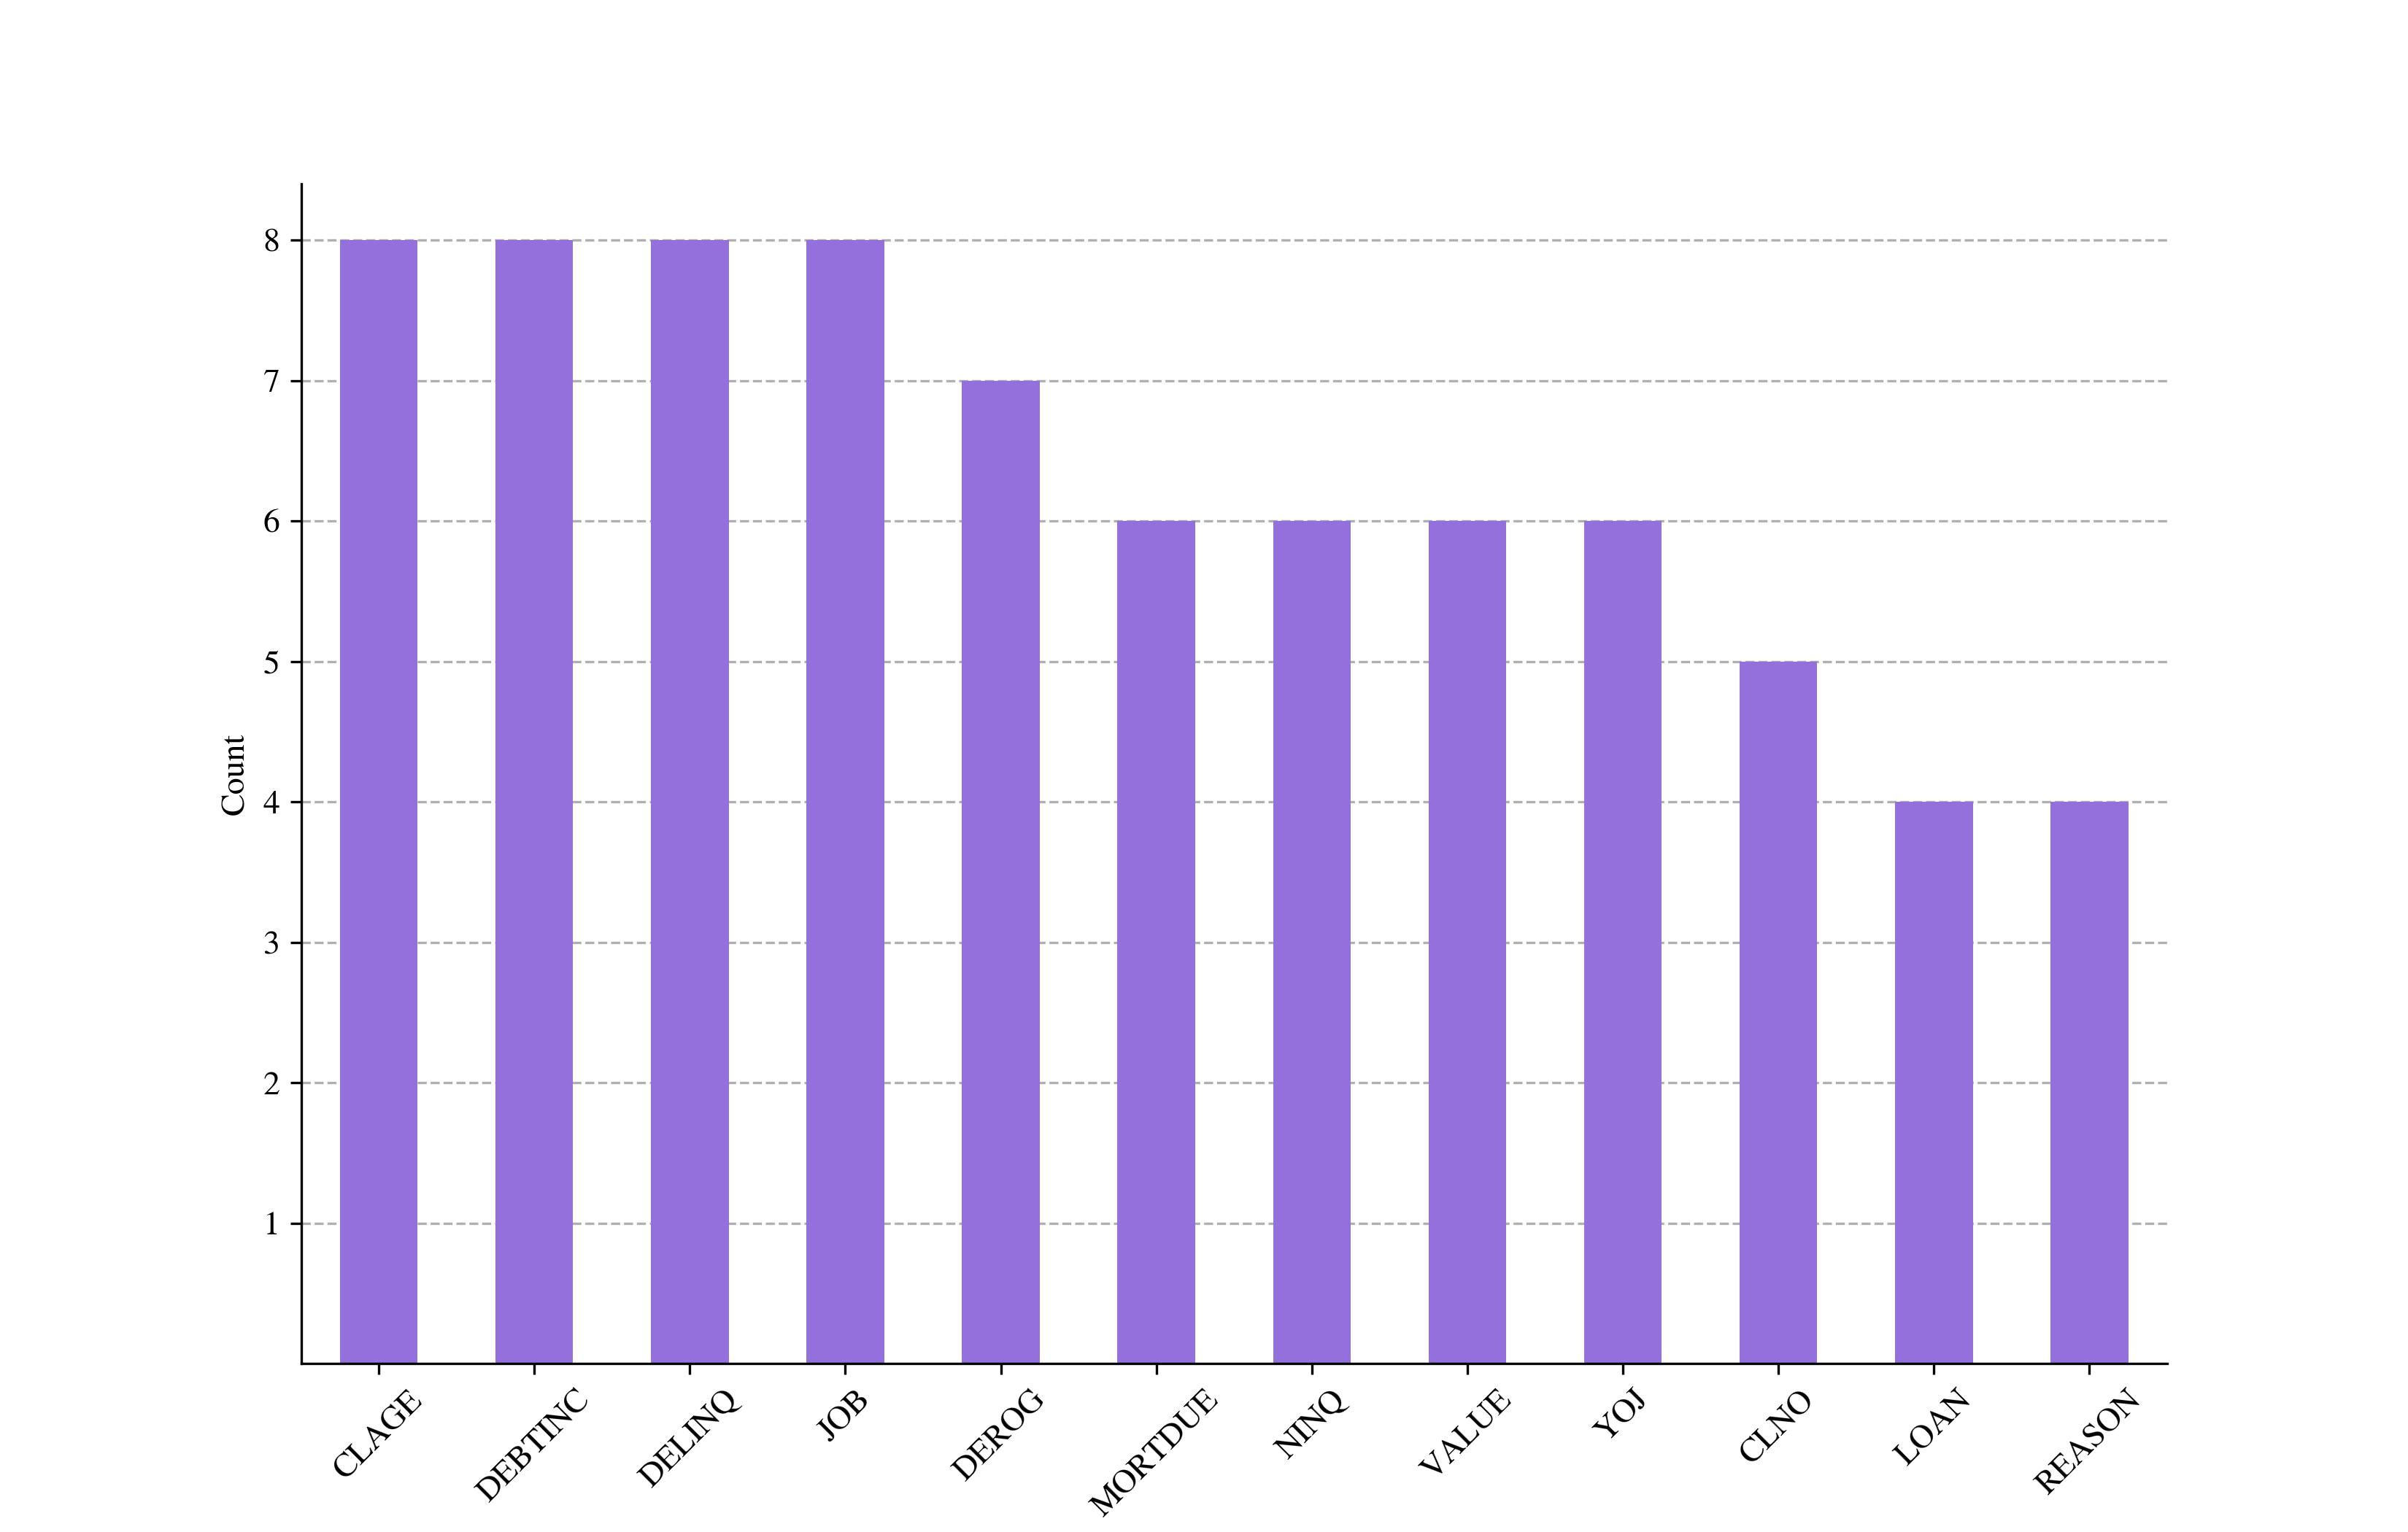
\includegraphics[width=120mm]{Figures/Recurrence_Selected_Features.jpg}

\centering{\begin{source}Author's results in Python\end{source}}\vspace{-1em}
\end{figure}


According to \autoref{fig:fsdistmod}, models such as KNN, Random Forest, Gradient Boosting and SVM chose almost all the features, as only one feature was eliminated. On the other hand, Gaussian Naive Bayes chose only 6. It seems that most of the features are important, as each model has selected a higher number of features.
It is evident that more complex black--box models require more features in contrast to transparent models such as Logistic Regression or Gaussian Naive Bayes.
\begin{figure}[H]
    \centering
    \caption{Distribution of Selected Features per Model}\vspace{0.5em}
    \label{fig:fsdistmod}\
    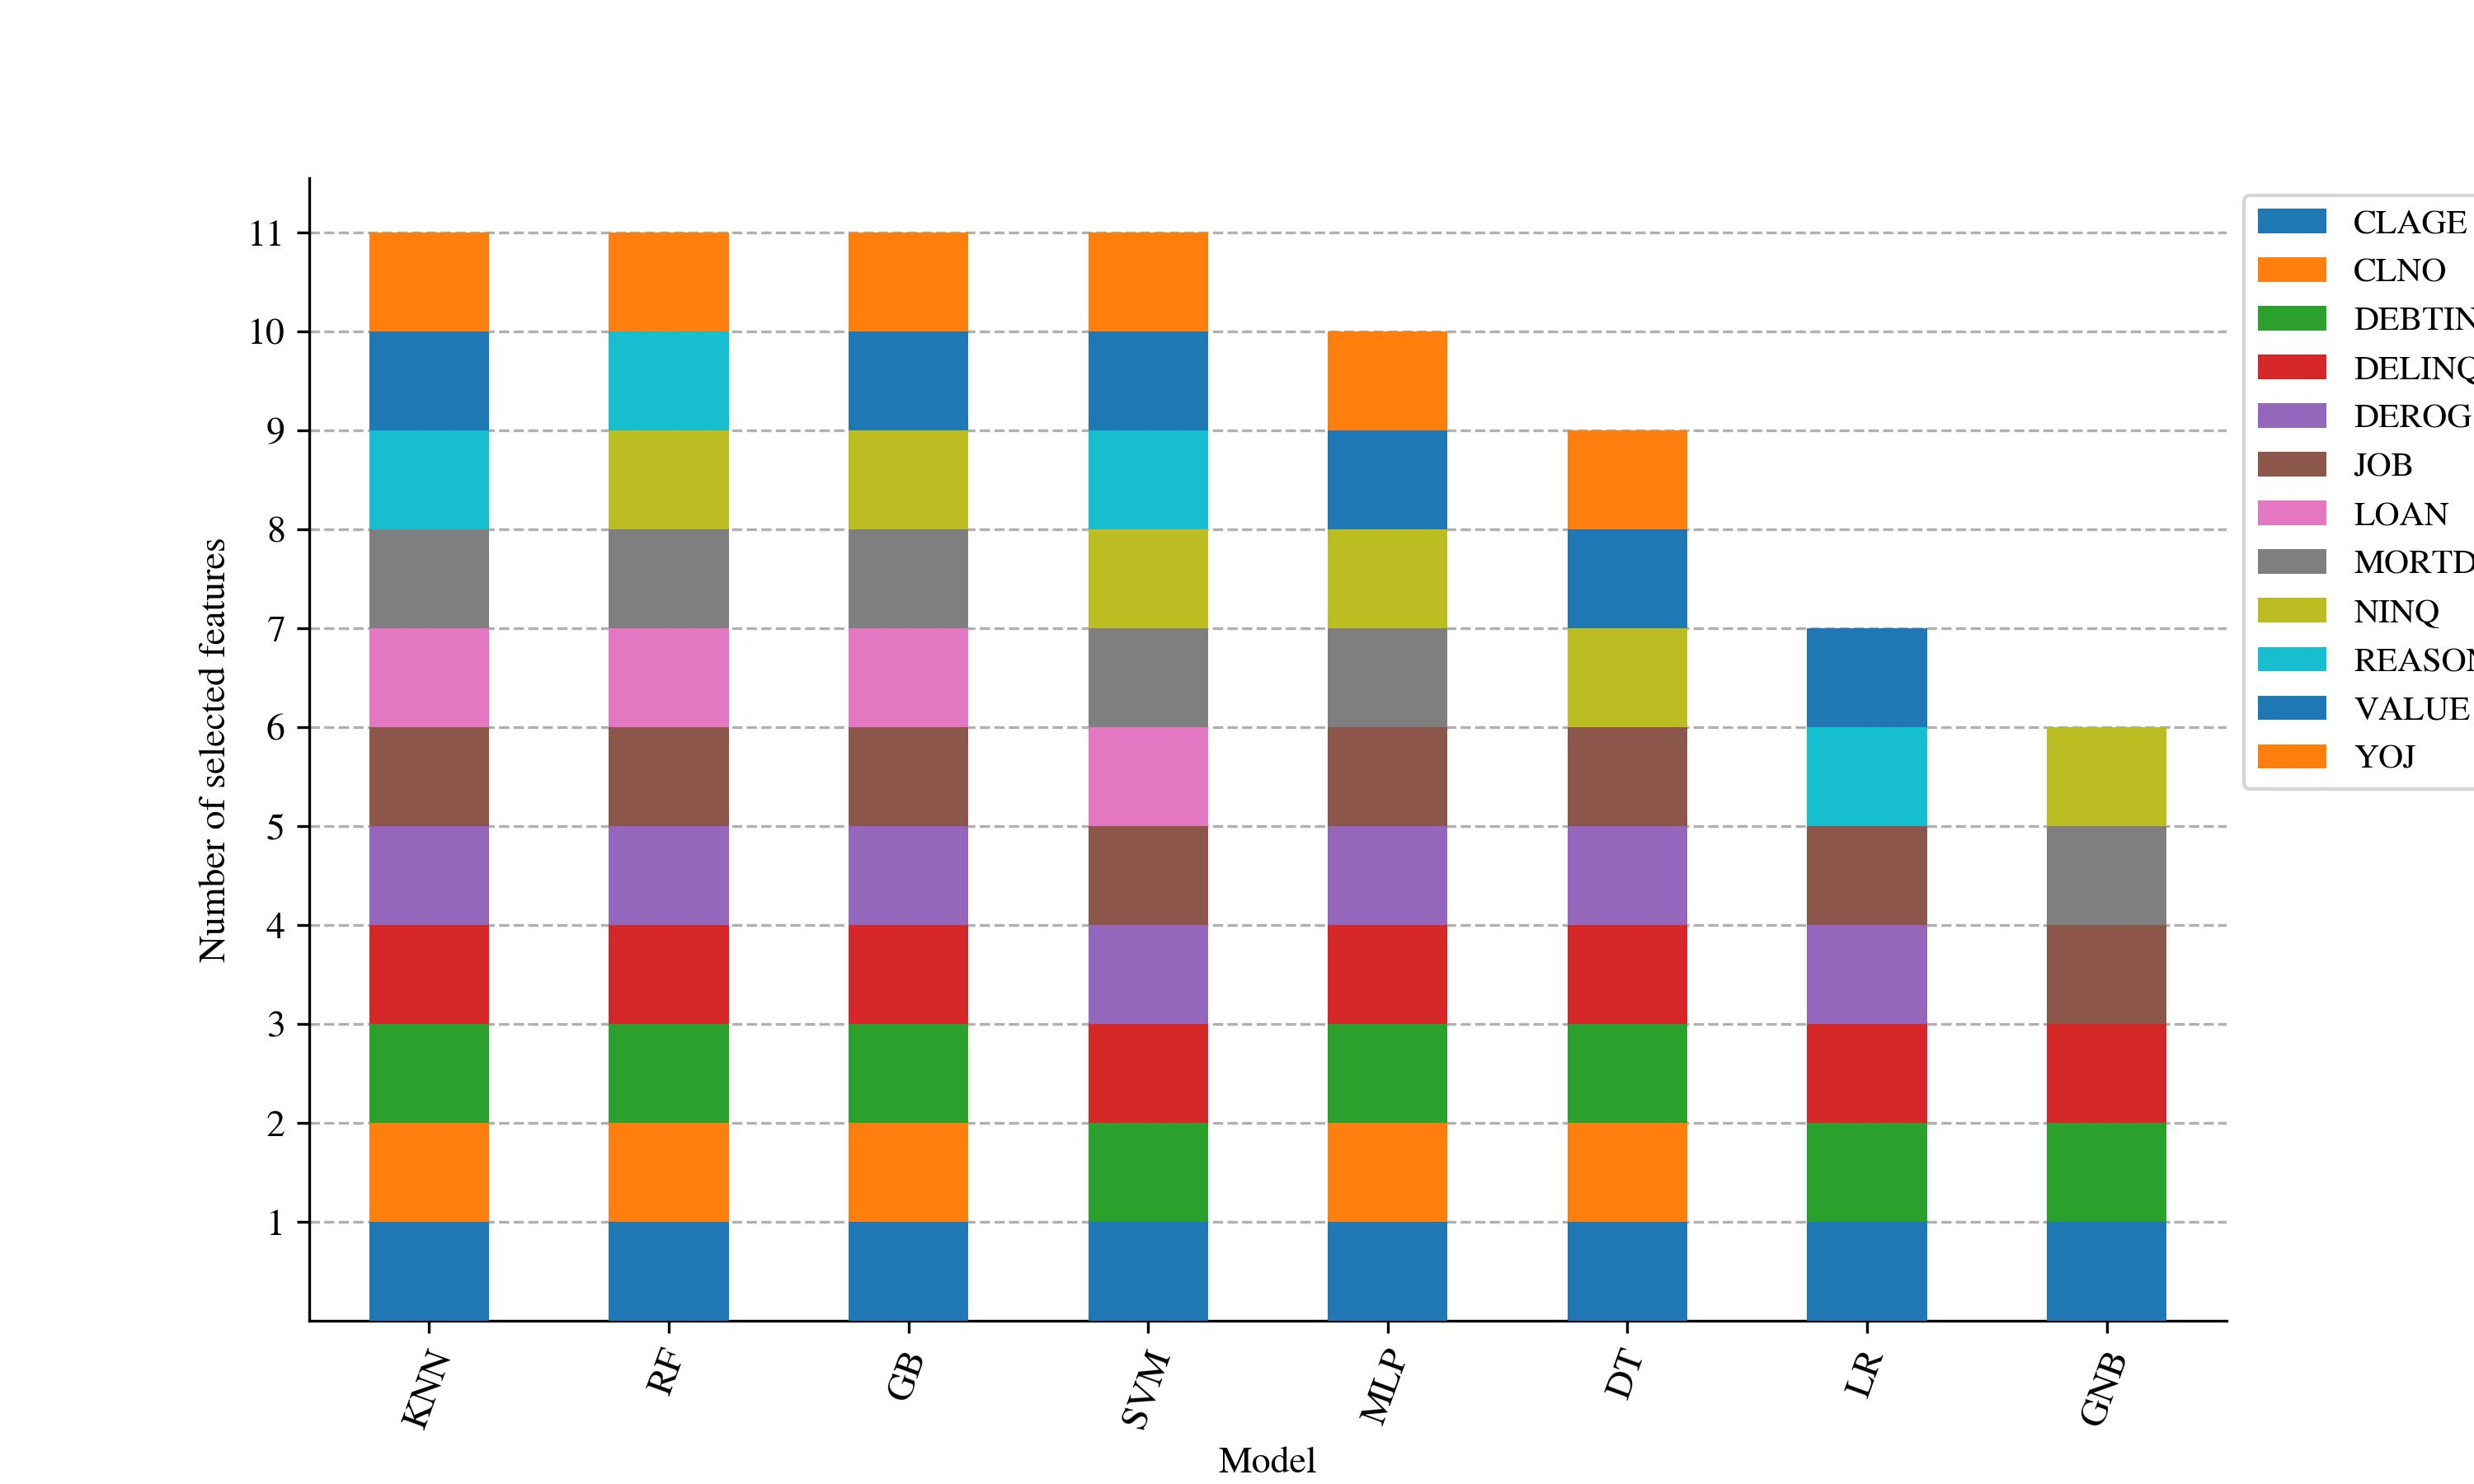
\includegraphics[width=120mm]{Figures/Selected_Features_Distribution.jpg}

    \centering{\begin{source}Author's results in Python\end{source}}\vspace{-1em}
\end{figure}

\newpage
\subsection{Model Selection}
\label{subsec:modelselection}

In combination with the pre--selected subsets of features, the next step regards the selection of the final model, which will be further used within an evaluation and deployment. The algorithm process is described in Algorithm \autoref{alg:model_selection} below:
\begin{algorithm}[H]
\caption{Model Selection Algorithm}
\label{alg:model_selection}
\begin{algorithmic}[1]
\For{$model \in \textit{models}$}
    \For{$features \in \textit{features\_subsets}$}
        \State $\textit{optimized\_model} \gets \textsc{BayesianOptimization}(model, features)$
        \For{$\textit{metric} \in \textit{evaluation\_metrics}$}
            \State $\textit{performance} \gets \textsc{Evaluation}(\textit{optimized\_model}, \textit{metric})$
        \EndFor
    \EndFor
\EndFor
\end{algorithmic}
\end{algorithm}


\vspace{-1em}
Hence, each input model is tuned on each subset of features selected within feature selection on the training set, and subsequently, the optimized model is evaluated on the validation set. Thus, when having $n$ input models and $m$ subsets of selected features, we get $n \times m$ tuned models.
$m \leq n$ because we exclude duplicated subsets of selected features, which can occur when more than one model chooses the same subset(s) of features.
Since there are 8 input models and 8 unique subsets of selected features, the total number of tuned models is 64.

\subsubsection{Metrics Ranking Space}

When evaluating classification models using class-based metrics such as F1 score, Precision, Recall, Accuracy, and Matthews Correlation Coefficient, a standard classification threshold of 0.5 is often used. This threshold separates predicted classes based on whether the predicted probability score is higher or lower than 0.5.
However, in real-world use cases, the 0.5 classification threshold may not be appropriate, and according to \citep{esposito2021ghost}, such threshold is not appropriate when having imbalanced data.

Therefore, it is recommended to calculate an optimal threshold rather than relying on the standard one.
In such case, the Youden index is employed, which is derived from the ROC curve and enables the selection of an optimal classification threshold value.
The Youden index searches for such threshold that maximizes the sum of True Positive Rate and True Negative Rate, decreased by 1 \citep{fluss2005estimation}, thus:
\begin{equation}\label{eq}
J = TPR + TNR - 1
\end{equation}
Mathematically, the optimal threshold using the Youden index is derived as follows:
\begin{equation}\label{eq}
T_{opt} = \text{argmax}_{t \in [0, 1]}\left(J\right)
\end{equation}
In Python, the \lstinline{roc_curve} function from \lstinline{Scikit-learn} returns False Positive Rate instead of the True Negative Rate. Nevertheless, we can derive the True Negative Rate from False Positive Rate as follows:
\begin{equation}\label{eq}
TNR =  1-FPR
\end{equation}
Therefore:
\begin{equation}\label{eq:youden}
T_{opt} = \text{argmax}_{t \in [0, 1]}\left(TPR +  \left(1-FPR\right) - 1\right)
\end{equation}
Note, that the optimal threshold is calculated based on the training set and henceforth applied within the evaluation of the validation set.

In order to ensure a more comprehensive and unbiased evaluation of a model's performance, it is recommended to consider multiple metrics rather than relying on a single metric alone. This approach provides a more generalized overview of the model's performance across different aspects and helps to prevent any bias towards a single metric.
To accomplish this, models can be ranked based on their performances on each individual metric, where a higher score or a lower loss indicates a better model, resulting in a higher rank for that metric.
Subsequently, for each model, a rank score is calculated in order to determine the final rank. The lower rank score indicates a better model's performance. For a particular model $M$, the rank score can be calculated as a weighted average of the individual ranks as follows:
\begin{equation}\label{eq:rankscorem}
    RankScore_{M} = \frac{\sum_{i=1}^{k} {r_i \times w_i}}{\sum_{i=1}^{k} {w_i}} 
\end{equation}
where $k$ is the number of metrics used to evaluated the model $M$, $r_i$ is the rank order of $i$--th metric for given model $M$ and $w_i$ is the weight assigned to the $i$--th metric.
Such metric lies in interval $<1, k>$, where 1 would indicate a perfect model' performance across the all metrics.
Based on the rank scores, we assign the final ranks where rank of 1 indicates the best performing model whereas rank $k$ determines the worst performing model.


The weights have been set expertly and are summarized in \autoref{tab:weightsrank}.
Specifically, the highest weight (1.5) is assigned to the F1 score, which provides a balanced measure of a model's performance with respect to both False Positives and False Negatives.
This metric is commonly used in classification tasks, particularly in imbalanced data sets, such as the validation set in our case, which has not been oversampled.
In addition to the F1 score, higher weight is assigned to the Recall score as well (1.2), which is a metric that penalizes False Negatives.
False Negatives occur when the model predicts a negative result (i.e., no default) for an instance that is actually positive (i.e., default).
In the context of loan applications, one may prefer to reject a loan applicant who would not have defaulted (False Positive) rather than approve the application of a client who would have defaulted (False Negative). Therefore, it is appropriate to give higher weight to Recall in order to reduce the likelihood of False Negatives.
Henceforth, the weights are assigned to different metrics based on their relevance to the models' ranking, with the highest weight given to F1 score and additional weight given to Recall to ensure that False Negatives are minimized.

\begin{table}[H]
\small
\setlength{\tabcolsep}{8pt}
\renewcommand{\arraystretch}{1.3}
\centering
    \caption[Model Ranking Weights]{Model Ranking Weights}\label{tab:weightsrank}
    \begin{tabular}{>{\raggedleft\arraybackslash}p{0.4\linewidth} l}
\toprule
\textbf{Metric} & \textbf{Weight}\\
\midrule
\hline
F1 score & 1.5 \\
Recall & 1.2 \\
Precision & 1 \\
Accuracy & 1 \\
AUC & 1 \\
Somers' D & 1 \\ 
Kolmogorov Smirnov & 1 \\
Matthews Correlation Coefficient  & 1 \\
Brier Score Loss  & 1 \\
\hline
\bottomrule
\end{tabular}
\vspace{0.7em}

\centering{\begin{source}Author's results in Python\end{source}}\vspace{-1em}
\end{table}




\newpage
\subsubsection{Model Selection Results}



The custom function \lstinline{model_selection()} iteratively prints the process of the model tuning and evaluation on each subset of features, in order to keep the track of such process as it is depicted in \autoref{fig:modselprint}.
Particularly, it prints which model on which features is being tuned and evaluated, execution time, optimal threshold, F1 score on the validation set, and the best hyperparameters.

\begin{figure}[H]
\centering\caption{Model Selection Print Statement}
\label{fig:modselprint}

{\fontsize{8.8}{11}\selectfont 
\begin{verbatim}
-------------------------------------------------------------------------------------
---------------------------------------- 7/64 ---------------------------------------
-------------------------------------------------------------------------------------
---------------------------- BAYESIAN OPTIMIZATION OF LR ----------------------------
--------------------------- WITH FEATURES SELECTED BY SVM ---------------------------
-------------------------------------------------------------------------------------
------------------------------------------------------------------------------------- 

1/2 ... Starting Bayesian Optimization on the subset of features (11 features):
        LOAN, MORTDUE, VALUE, REASON, JOB, YOJ, DEROG, DELINQ, CLAGE, NINQ, DEBTINC
2/2... Bayesian Optimization finished 

Execution time: 1.493 minutes 

F1 Score on Validation set: 0.6160919540229886 

Optimal classification threshold: 0.4003

Tuned hyperparameters of LR: 

        C: 0.2768320429063577
        class_weight: balanced
        dual: False
        fit_intercept: True
        intercept_scaling: 25.603205585229382
        l1_ratio: 0.5230523280543836
        max_iter: 100
        multi_class: auto
        n_jobs: -1
        penalty: elasticnet
        random_state: 42
        solver: saga
        tol: 0.0001
        verbose: 0
        warm_start: False
-------------------------------------------------------------------------------------
-------------------------------------------------------------------------------------
\end{verbatim}
}
\centering{\begin{source}Author's results in Python\end{source}}\vspace{0em}
\end{figure}


\newpage



The final output of the function \lstinline{model_selection()} is a table that summarizes the model's computed metrics as depicted in \autoref{tab:modelsectab}.
For a reference \textbf{Tuned model} refers to the model over which the model selection algorithm is iterated, \textbf{FS model} refers to the model that was used as an input estimator in Forward SFS in order to select a subset of optimal features,
\textbf{\# Features} refers to the number of selected features on which the model is tuned, \textbf{Exec. Time} refers to the optimalization and training time of the tuned model, and \textbf{Thres.} refers to the optimal threshold computed by the Youden index (\autoref{eq:youden}).


The next columns represent the evaluation metrics, namely F1 score (\textbf{F1}), Precision (\textbf{Prec.}), Recall (\textbf{Rec.}), Accuracy (\textbf{Acc.}), AUC, Somers' D (\textbf{SD}), Kolmogorov-Smirnov Distance (\textbf{KS}), Matthews Correlation Coefficient (\textbf{MCC}), Brier Score Loss (\textbf{BS}), and Log Loss.
The last two columns represent the rank score of the model computed according to \autoref{eq:rankscorem} (\textbf{Score}), and the last column (\textbf{Rank}) is the final rank based on which we determine the final model.


As can be seen, the best models in terms of ranking are the Gradient Boosting models, which in general have the highest score metrics and the lowest loss metrics, followed by another ensemble mode, Random Forest.
On the other hand, the worst-performing models are Gaussian Naive Bayes models. In the first ten worst performing models, we can also observe that Decision Tree and Logistic Regression, as white--box models, perform poorly.

\clearpage
\newpage

\KOMAoptions{paper=landscape,DIV=last}
\newgeometry{hmargin=2.5cm,bottom=25mm,height=150mm,includehead}
\fancyheadoffset{0pt}



\begin{table}[H]
\small
\setlength{\tabcolsep}{8pt}
\renewcommand{\arraystretch}{1.3}
\caption[Model Selection Results]{Model Selection Results}\label{tab:modelsectab}
\centering
\scalebox{0.8}{

\begin{tabular}{|p{1.3cm}|p{1.3cm}|>{\raggedleft}p{1.5cm}|>{\raggedleft}p{1.3cm}|c|c|c|c|c|c|c|c|c|c|c|c||c|c|}
    \toprule
    \textbf{Tuned model} & \textbf{FS model} & \textbf{\# \newline Features} & \textbf{Exec. \newline Time} & \textbf{Thresh.} & \textbf{F1} & \textbf{Prec.} & \textbf{Rec.} & \textbf{Acc.} & \textbf{AUC} & \textbf{SD} & \textbf{KS} & \textbf{MCC} & \textbf{BS} & \textbf{Log Loss} & \textbf{Score} & \textbf{Rank} \\
    \midrule
    \hline
    GB & MLP & 10 & 12.57 & 0.4955 & 0.7809 & 0.7853 & 0.7765 & 0.9128 & 0.9515 & 0.9030 & 0.7751 & 0.7265 & 0.0666 & 0.2487 & 3.30 & 1 \\
    GB & RF & 11 & 14.10 & 0.4973 & 0.7775 & 0.7841 & 0.7709 & 0.9117 & 0.9541 & 0.9081 & 0.7961 & 0.7225 & 0.0669 & 0.2803 & 3.97 & 2 \\
    GB & KNN & 11 & 14.18 & 0.5072 & 0.7978 & 0.7912 & 0.8045 & 0.9184 & 0.9587 & 0.9175 & 0.7989 & 0.7467 & 0.0687 & 0.4135 & 4.08 & 3 \\
    GB & SVM & 11 & 15.33 & 0.5053 & 0.7896 & 0.8155 & 0.7654 & 0.9184 & 0.9555 & 0.9109 & 0.7961 & 0.7397 & 0.0718 & 0.3486 & 4.32 & 4 \\
    GB & GB & 11 & 11.86 & 0.4132 & 0.7799 & 0.7778 & 0.7821 & 0.9117 & 0.9543 & 0.9086 & 0.7989 & 0.7247 & 0.0703 & 0.3372 & 4.39 & 5 \\
    RF & KNN & 11 & 6.01 & 0.4725 & 0.7486 & 0.7326 & 0.7654 & 0.8972 & 0.9226 & 0.8452 & 0.7109 & 0.6843 & 0.0923 & 0.3232 & 8.48 & 6 \\ 
    GB & DT & 9 & 12.91 & 0.4729 & 0.7675 & 0.7697 & 0.7654 & 0.9073 & 0.9407 & 0.8814 & 0.7556 & 0.7096 & 0.0808 & 0.4693 & 8.80 & 7 \\ 
    RF & GB & 11 & 5.18 & 0.4517 & 0.7385 & 0.7135 & 0.7654 & 0.8916 & 0.9200 & 0.8400 & 0.7123 & 0.6709 & 0.0886 & 0.3135 & 9.22 & 8 \\ 
    RF & MLP & 10 & 6.72 & 0.4761 & 0.7357 & 0.7181 & 0.7542 & 0.8916 & 0.9179 & 0.8358 & 0.7081 & 0.6679 & 0.0879 & 0.3084 & 10.20 & 9 \\
    GB & LR & 7 & 17.58 & 0.4362 & 0.7388 & 0.7000 & 0.7821 & 0.8894 & 0.9219 & 0.8438 & 0.7081 & 0.6706 & 0.0886 & 0.3925 & 11.03 & 10 \\ 
\ldots & \ldots & \ldots & \ldots & \ldots & \ldots & \ldots & \ldots & \ldots & \ldots & \ldots & \ldots & \ldots & \ldots & \ldots & \ldots & \ldots \\
GNB & DT & 9 & 0.40 & 0.2241 & 0.6063 & 0.5095 & 0.7486 & 0.8056 & 0.8467 & 0.6935 & 0.5768 & 0.4991 & 0.1316 & 0.6370 & 49.56 & 55 \\ 
GNB & MLP & 10 & 0.39 & 0.2194 & 0.6013 & 0.5000 & 0.7542 & 0.8000 & 0.8493 & 0.6986 & 0.5768 & 0.4930 & 0.1319 & 0.6360 & 49.68 & 56 \\ 
GNB & KNN & 11 & 0.35 & 0.3588 & 0.6093 & 0.5219 & 0.7318 & 0.8123 & 0.8479 & 0.6957 & 0.5698 & 0.5024 & 0.1367 & 0.6686 & 50.58 & 57 \\ 
DT & MLP & 10 & 0.87 & 0.5000 & 0.6427 & 0.6374 & 0.6480 & 0.8559 & 0.8133 & 0.6266 & 0.5810 & 0.5524 & 0.1254 & 2.0008 & 52.10 & 58 \\ 
SVM & GNB & 6 & 6.66 & 0.1821 & 0.5788 & 0.4718 & 0.7486 & 0.7821 & 0.8393 & 0.6786 & 0.5768 & 0.4633 & 0.1355 & 0.4354 & 53.11 & 59 \\ 
DT & GNB & 6 & 0.85 & 0.5000 & 0.6354 & 0.6284 & 0.6425 & 0.8525 & 0.8187 & 0.6375 & 0.5838 & 0.5430 & 0.1251 & 2.1679 & 53.31 & 60 \\ 
GNB & SVM & 11 & 0.36 & 0.1991 & 0.5885 & 0.4872 & 0.7430 & 0.7922 & 0.8425 & 0.6850 & 0.5712 & 0.4756 & 0.1345 & 0.6721 & 53.65 & 61 \\ 
GNB & GNB & 6 & 0.36 & 0.4787 & 0.5950 & 0.5039 & 0.7263 & 0.8022 & 0.8356 & 0.6711 & 0.5559 & 0.4835 & 0.1470 & 0.5280 & 53.79 & 62 \\ 
LR & GNB & 6 & 1.55 & 0.4561 & 0.5948 & 0.5121 & 0.7095 & 0.8067 & 0.8379 & 0.6758 & 0.5531 & 0.4831 & 0.1319 & 0.4180 & 54.02 & 63 \\ 
GNB & RF & 11 & 0.36 & 0.3413 & 0.5864 & 0.4943 & 0.7207 & 0.7966 & 0.8288 & 0.6577 & 0.5545 & 0.4720 & 0.1486 & 0.7040 & 57.08 & 64 \\ 
    \hline
    \bottomrule 
\end{tabular}}
\vspace{1em}

\centering{\begin{source}Author's results in Python\end{source}}\vspace{-1em}
\end{table}

\clearpage
\newpage
\KOMAoptions{paper=portrait,DIV=last}
\restoregeometry
\fancyheadoffset{0pt}

In order to gain a more detailed understanding of the model selection results, the distribution of computed metrics is plotted. In \autoref{fig:f1dist}, the F1 score distribution is visualized for each input model. An outlier can be observed in KNN where the F1 score is 0.			
\begin{figure}[H]
\centering
\caption{F1 Score Distribution}\vspace{0.5em}
\label{fig:f1dist}\
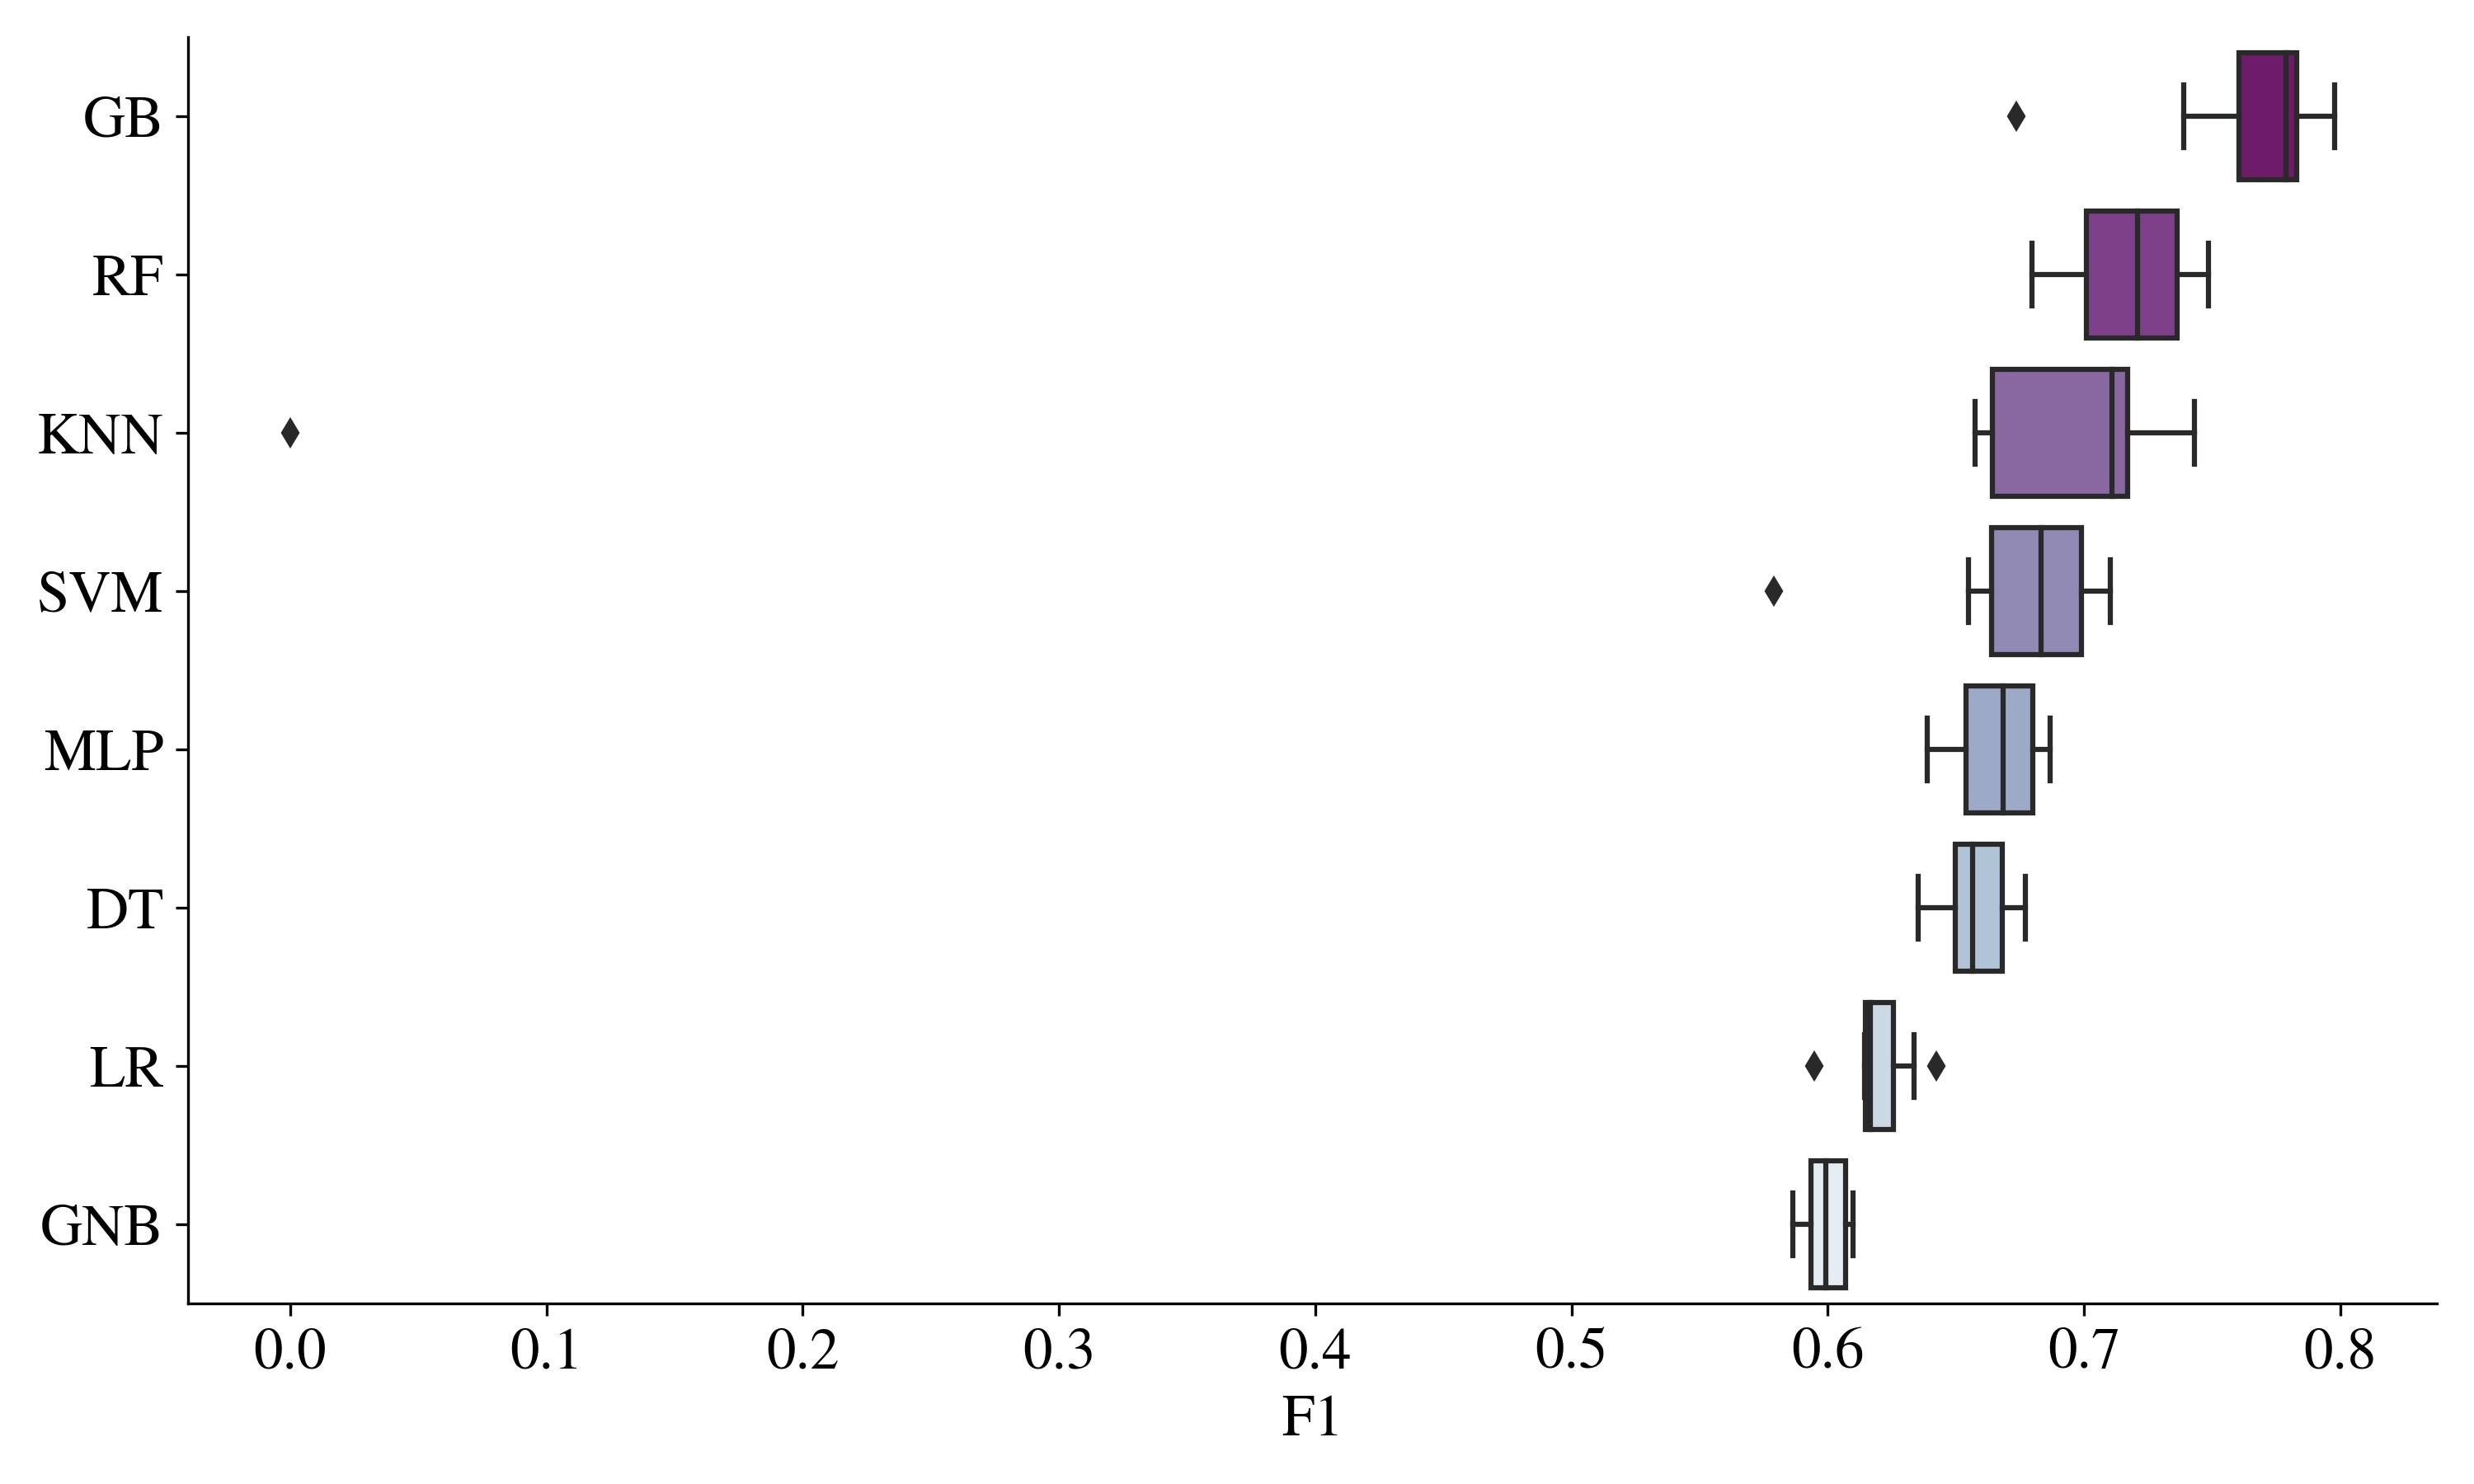
\includegraphics[width=140mm]{Figures/F1_Distribution.jpg}

\centering{\begin{source}Author's results in Python\end{source}}\vspace{-1em}
\end{figure}
\newpage
Such outlier is removed in \autoref{fig:f1distclean} to gain a more general insight into the F1 score distribution.
It can be observed that Gradient Boosting models have the highest F1 scores of around 80 \%.
Another tree ensemble model, Random Forest, is performing well as the second best. However, more transparent models such as Logistic Regression and Naive Bayes are performing poorly, having F1 scores around 60 \%.
\begin{figure}[H]
\centering
\caption{F1 Score Distribution - \textit{without outlier}}\vspace{0.5em}
\label{fig:f1distclean}\
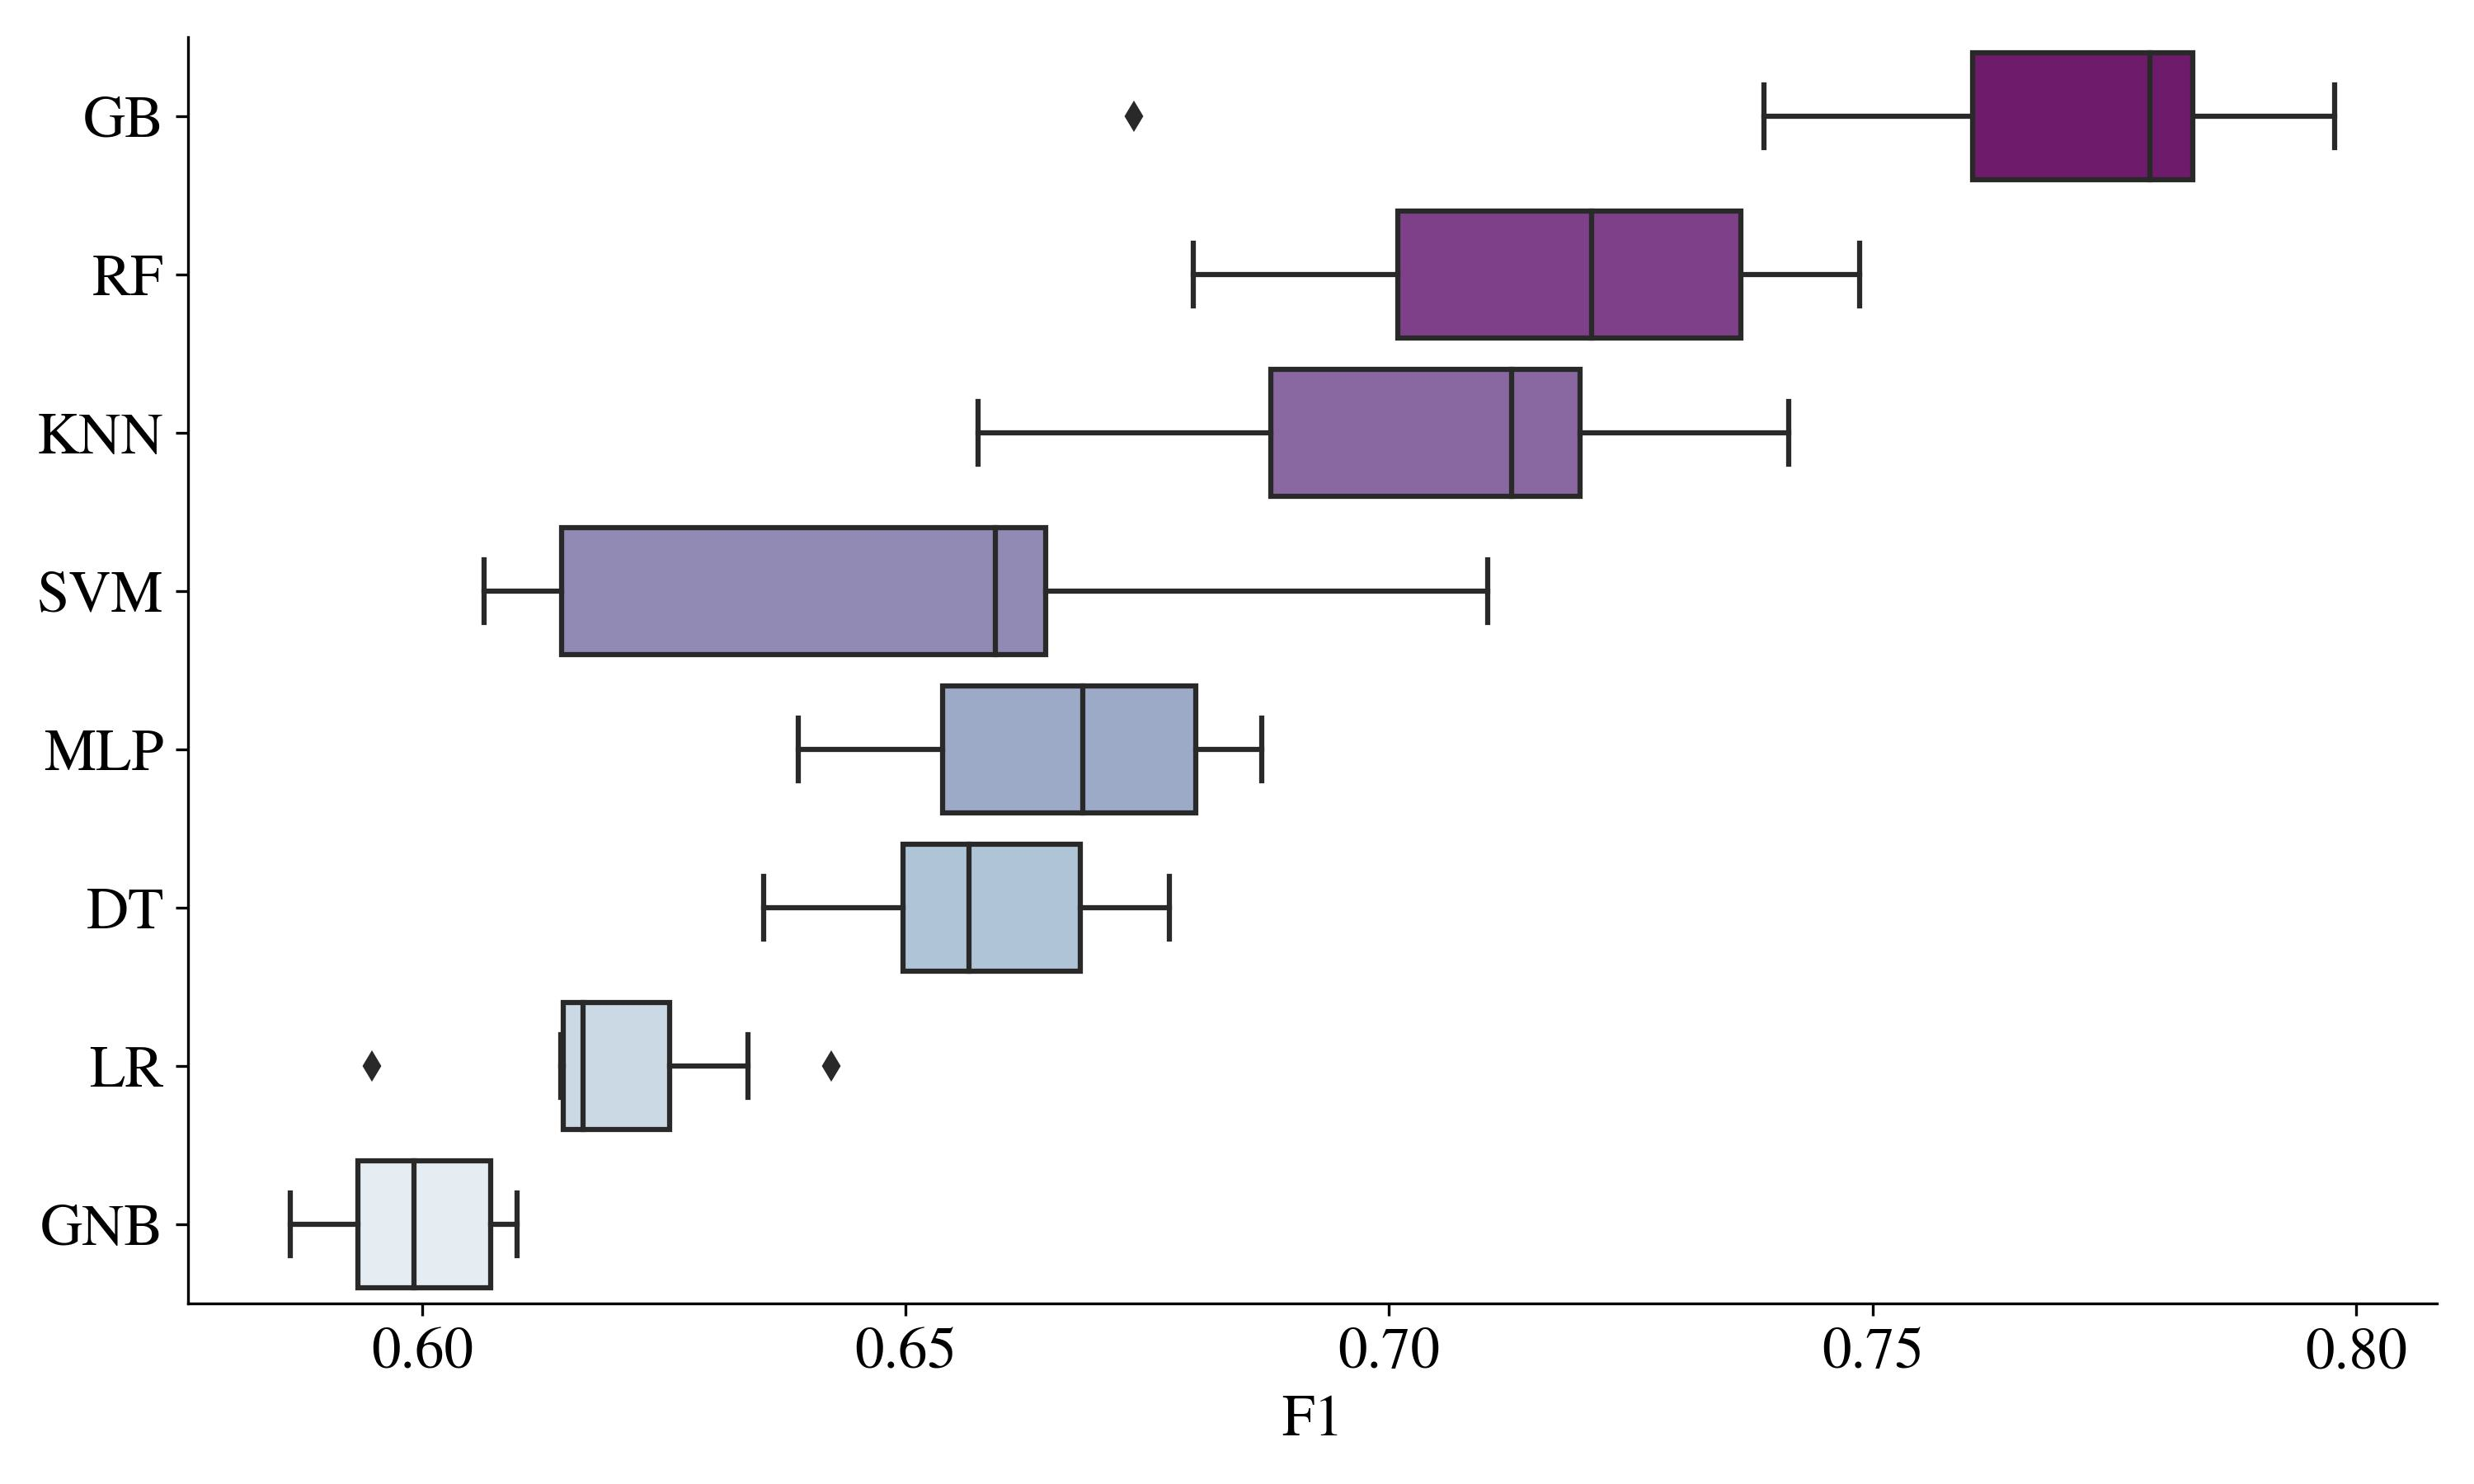
\includegraphics[width=140mm]{Figures/F1_wo_outliers_Distribution.jpg}

\centering{\begin{source}Author's results in Python\end{source}}\vspace{-1em}
\end{figure}
\newpage
As depicted in \autoref{fig:f1distcleanbbwb}, it visualizes the distribution of F1 score (without the outlier) across the model type. Although, both score distributions overlap, it is evident, that black--box models outperform white--box models in terms of F1 score in overall as expected.
\begin{figure}[H]
    \centering
    \caption{F1 Score Distribution (Black--box/White--box dimension) - \textit{without outlier}}\vspace{0.5em}
    \label{fig:f1distcleanbbwb}\
    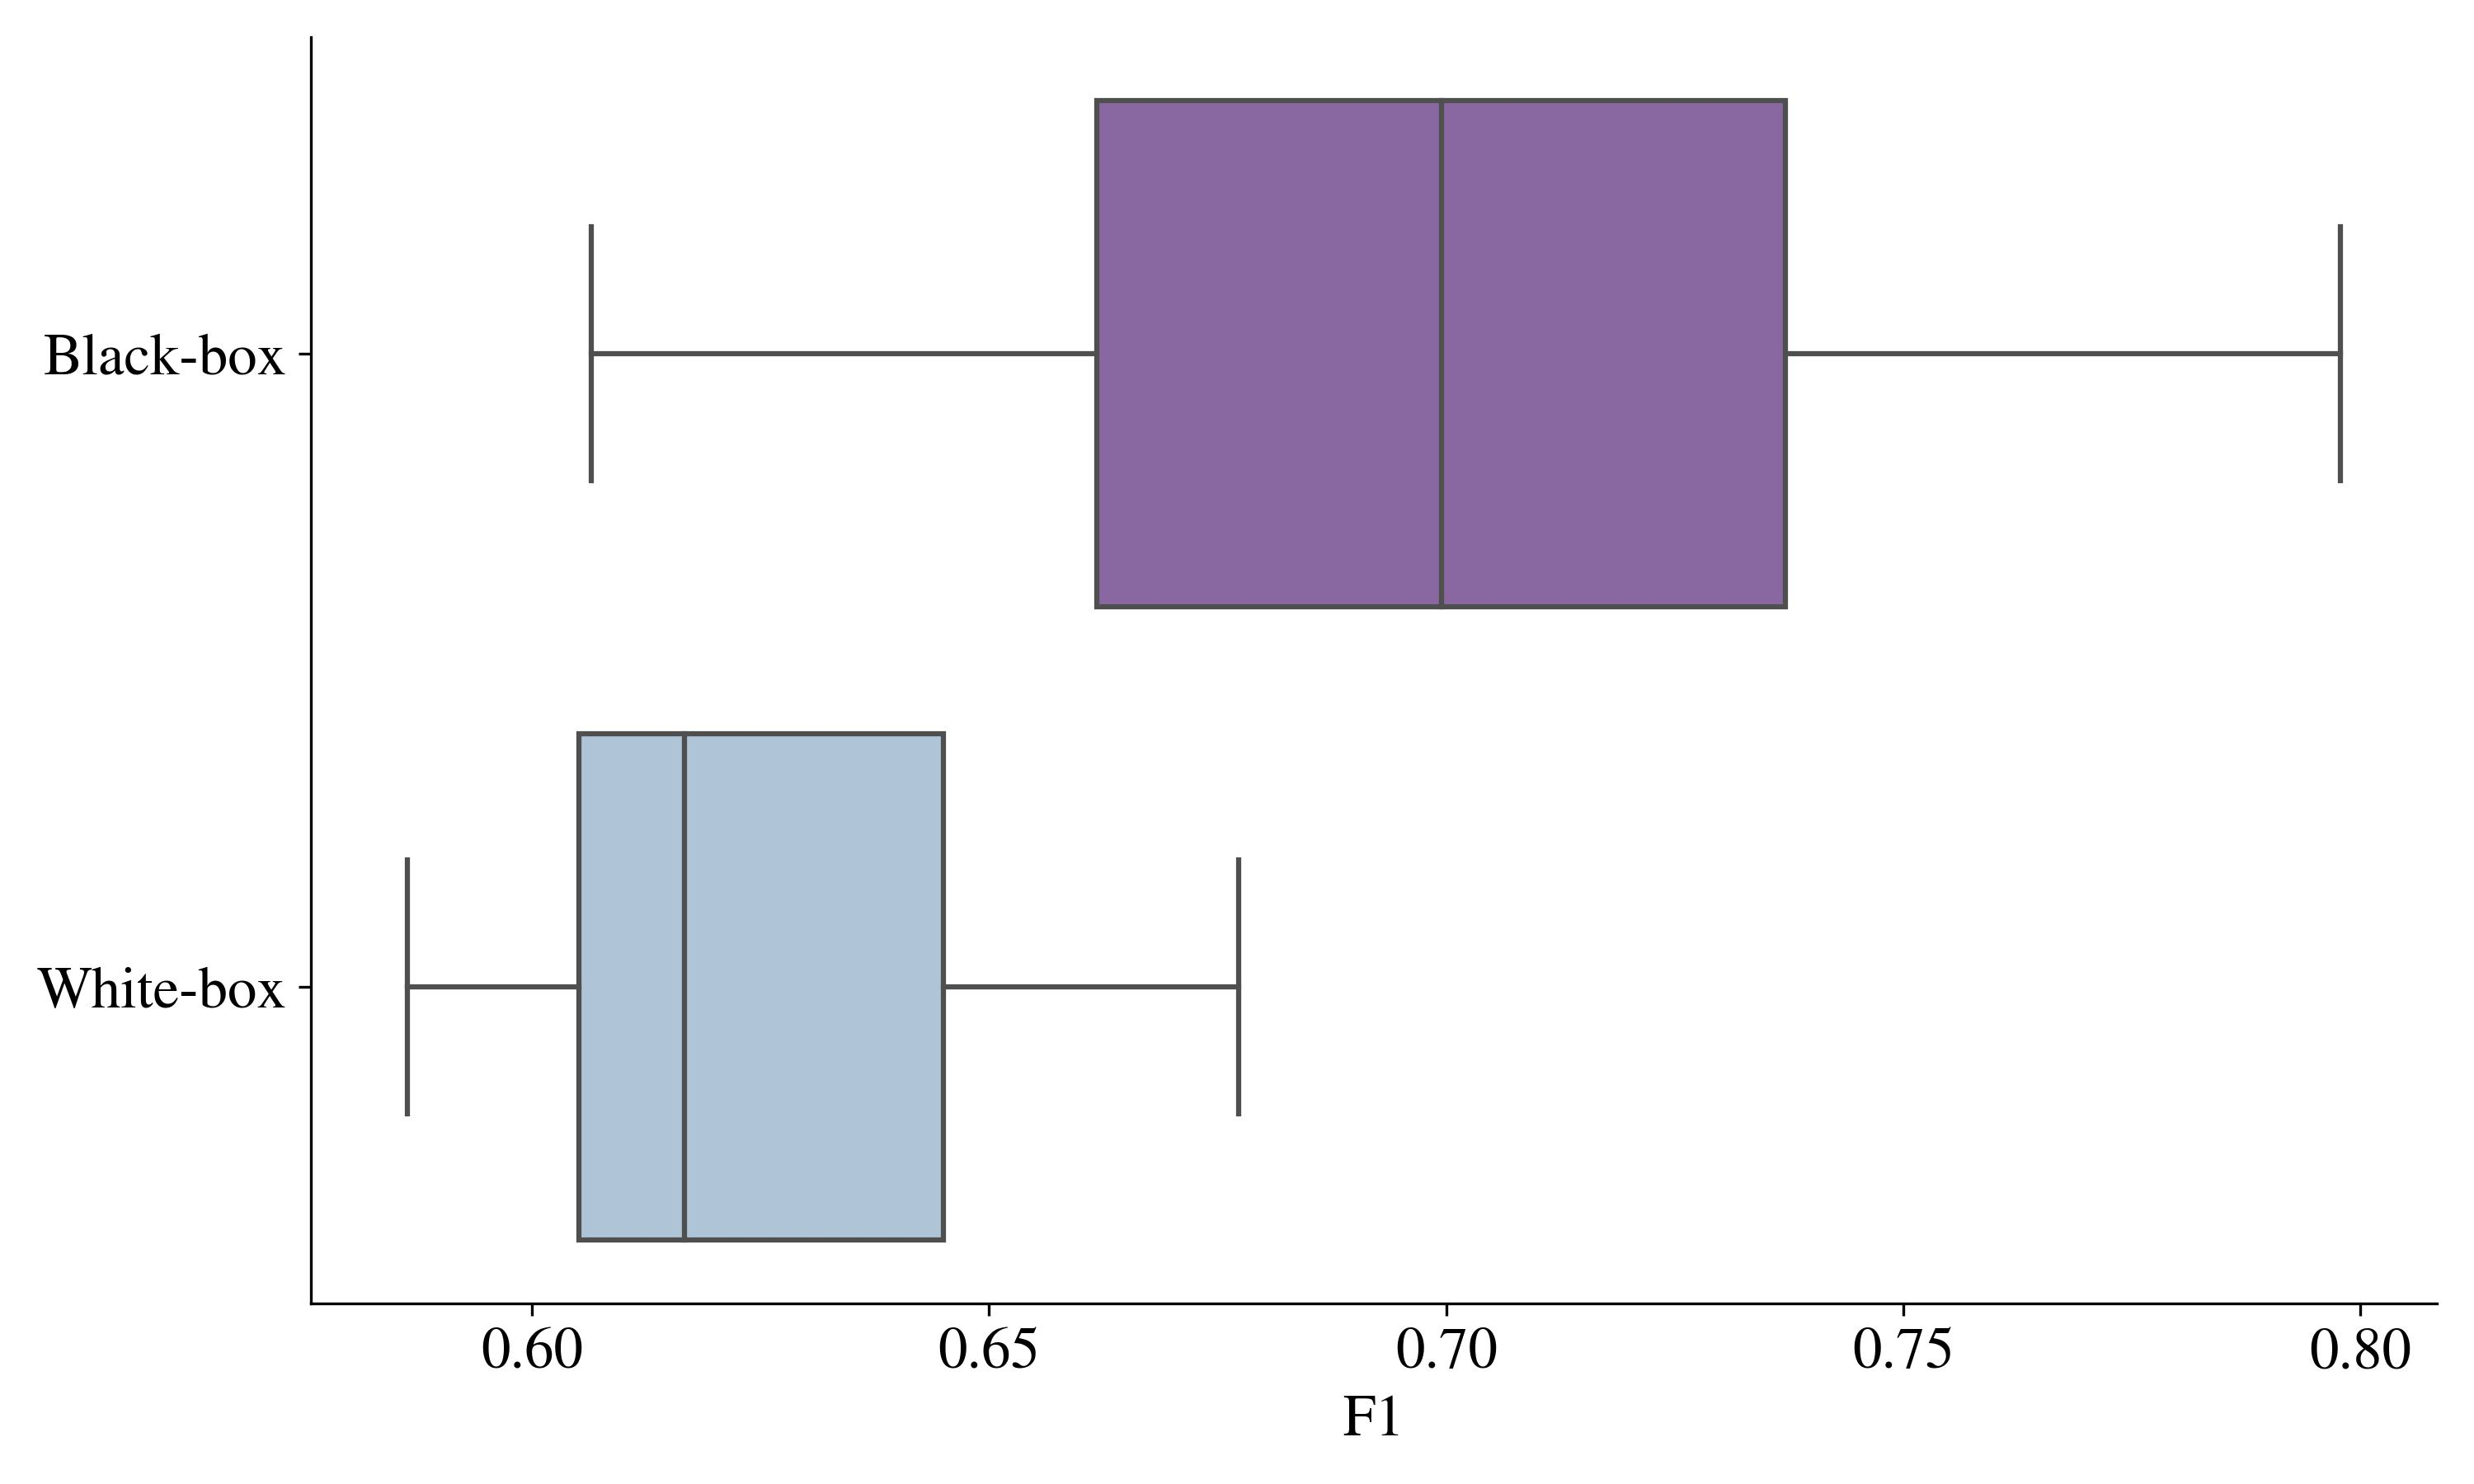
\includegraphics[width=140mm]{Figures/F1_wo_outliers_Distribution_BB_WB.jpg}

    \centering{\begin{source}Author's results in Python\end{source}}\vspace{-1em}
\end{figure}

\newpage
We can also consider not only the F1 score but also other metrics, which is quantified in the rank score calculated according to \autoref{eq:rankscorem}. As shown in \autoref{fig:avgrankdist}, we can observe that the order of models ranked by the rank score is identical as the order of the models ranked by the F1 score in \autoref{fig:f1dist}.
Hence, across all the metrics, the Gradient performs the best in overall while Gaussian Naive Bayes does not perform well at all.
\begin{figure}[H]
    \centering
    \caption{Rank Score Distribution}\vspace{0.5em}
    \label{fig:avgrankdist}\
    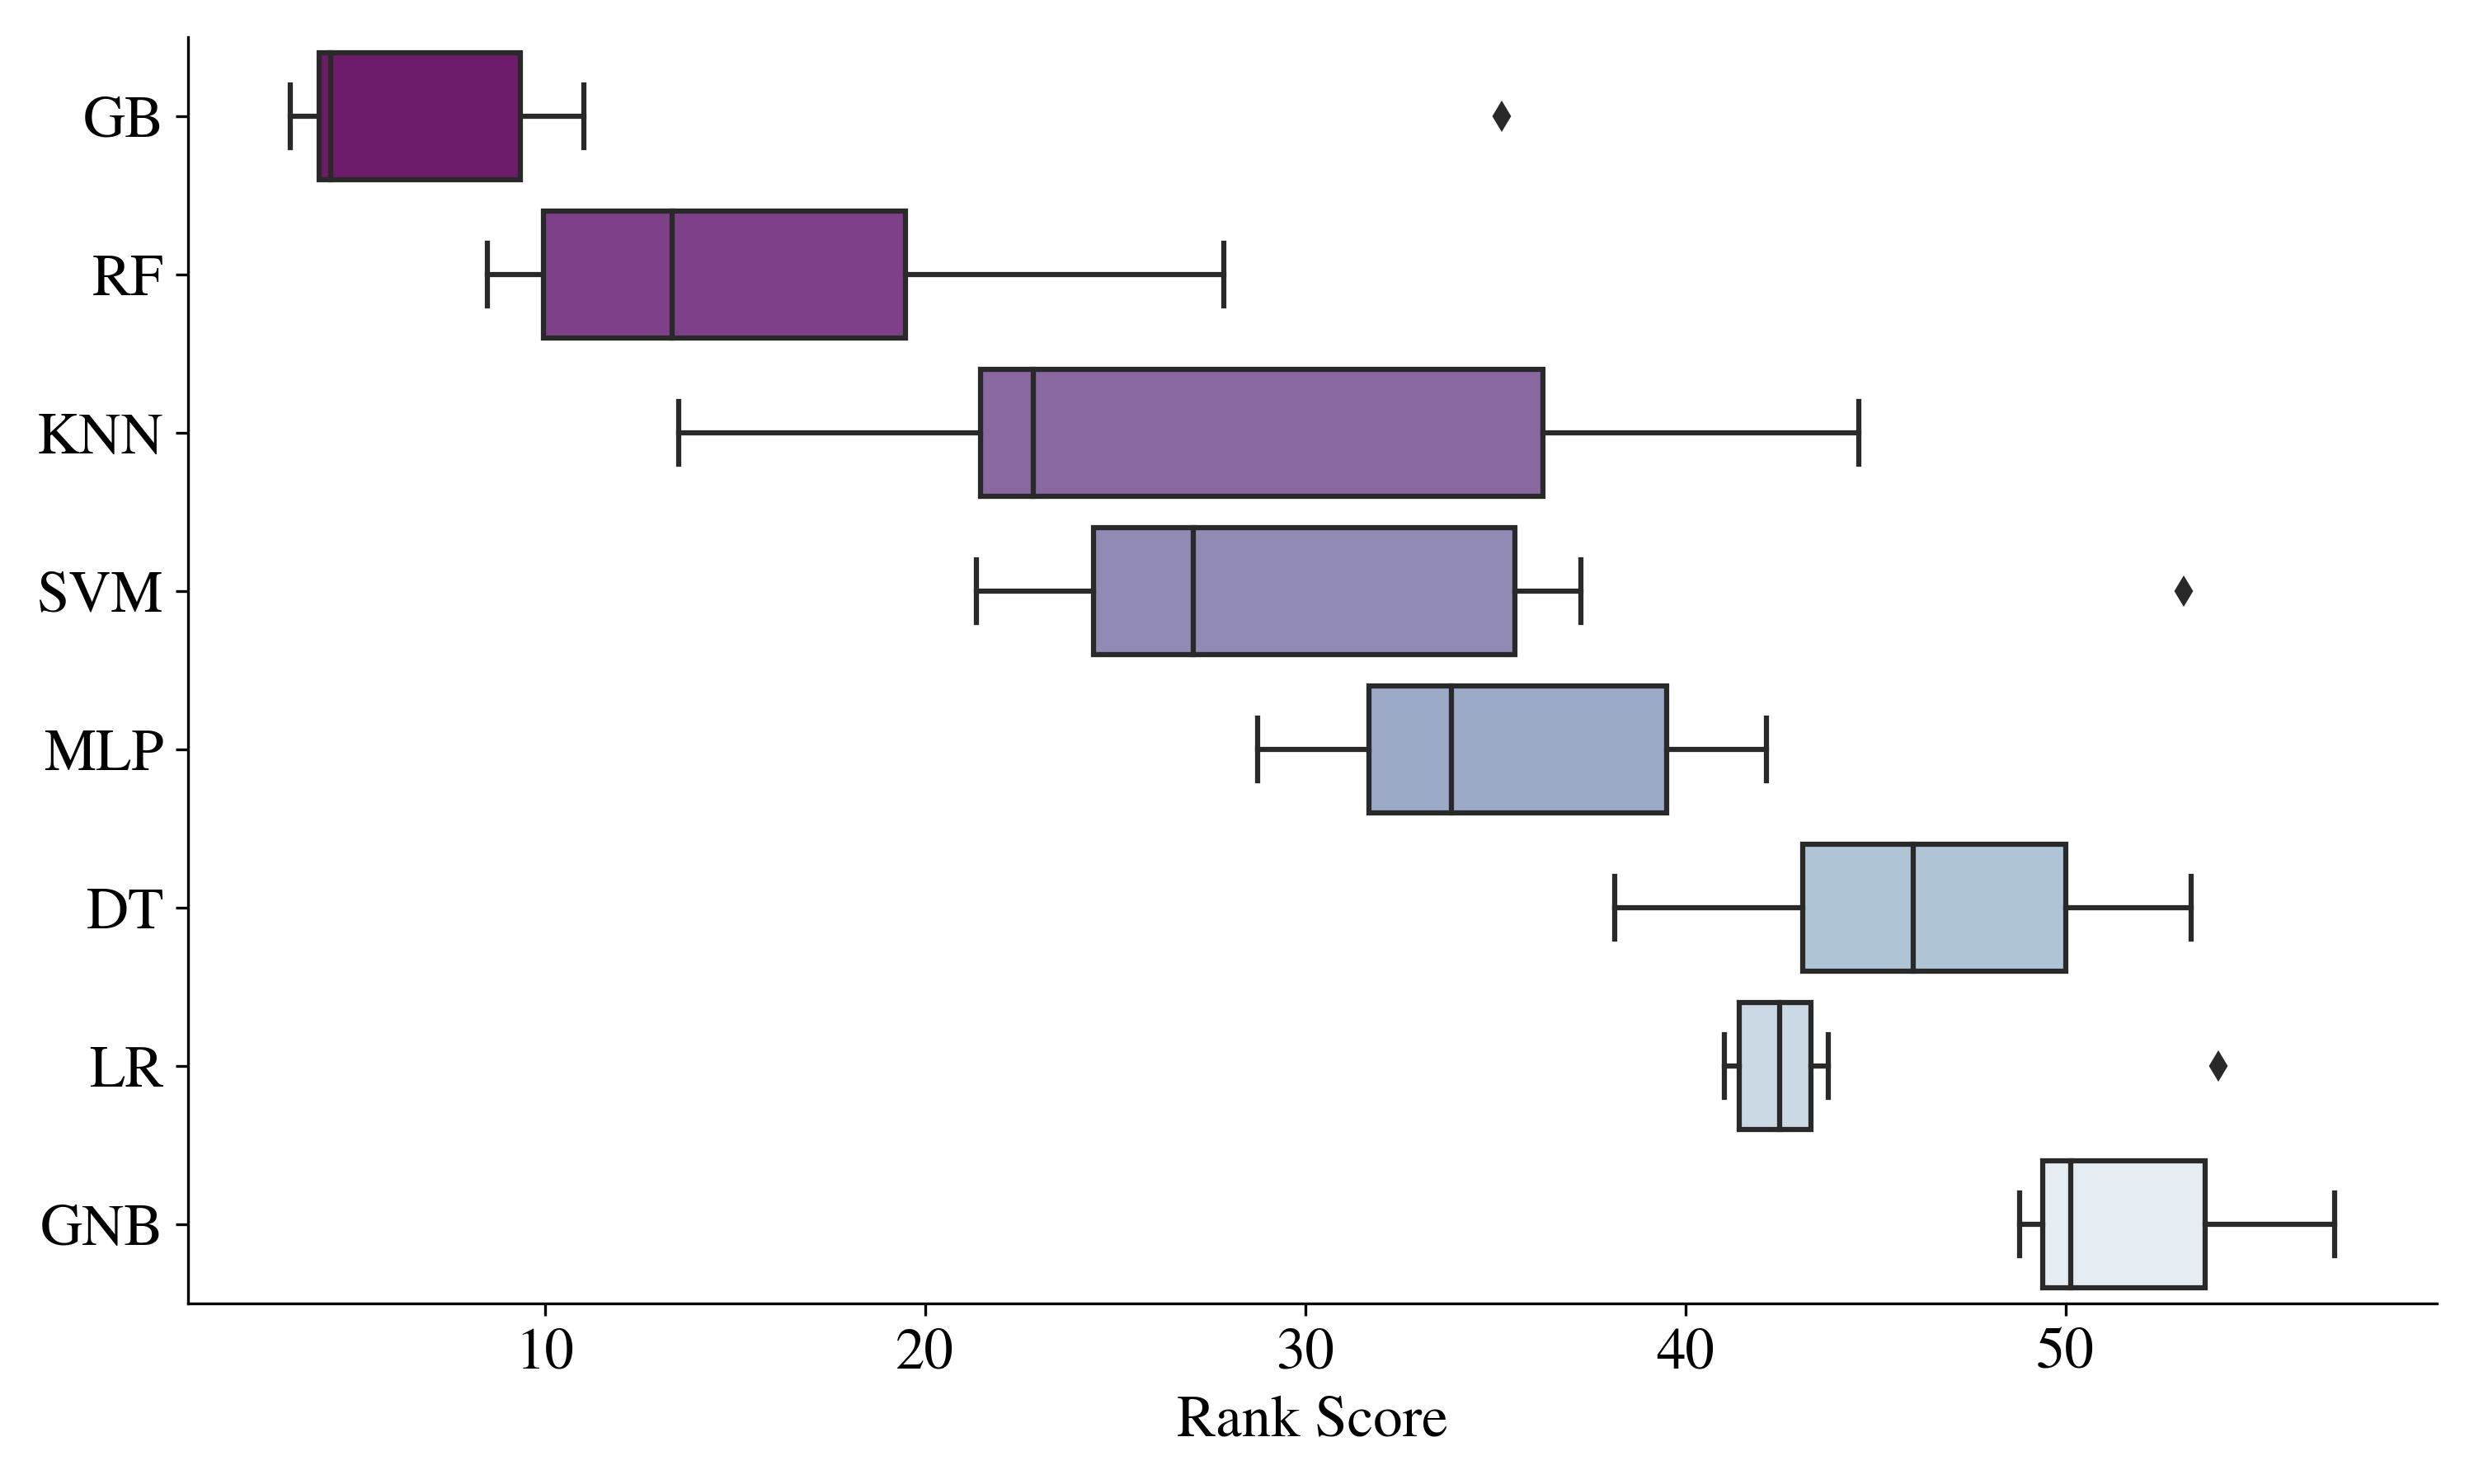
\includegraphics[width=140mm]{Figures/AVG_RANK_Distribution.jpg}

    \centering{\begin{source}Author's results in Python\end{source}}\vspace{-1em}
\end{figure}

\newpage
As expected, also, the black--box models are ranked higher than the white--box models according to the rank score as shown in \autoref{fig:avgrankdistbbwb}. This is evident also from \autoref{tab:modelsectab} where the black--box models, namely Gradient Boosting and Random Forest, dominated amongst the first 10 ranked models.
Other metrics' distribution analyses are shown in \autoref{sec:app1modelselectionresultsapp} in \autoref{chap:app1}.
\begin{figure}[H]
    \centering
    \caption{Rank Score Distribution (Black--box/White--box dimension)}\vspace{0.5em}
    \label{fig:avgrankdistbbwb}\
    \includegraphics[width=140mm]{Figures/AVG_Rank_Distribution_BB_WB.jpg}
    \centering{\begin{source}Author's results in Python\end{source}}\vspace{-1em}
\end{figure}

\newpage
The optimal threshold distribution for each base model is presented in \autoref{fig:thresdist}. We can observe an outlier in KNN having a threshold value of 1, which explains the F1 score outlier found previously in \autoref{fig:f1dist}.
\begin{figure}[H]
\centering
\caption{Threshold Distribution}\vspace{0.5em}
\label{fig:thresdist}\
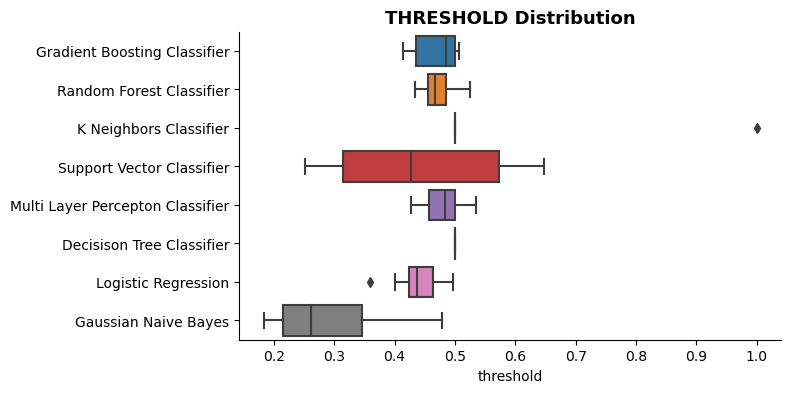
\includegraphics[width=140mm]{Figures/Threshold_Distribution.jpg}
\centering{\begin{source}Author's results in Python\end{source}}\vspace{-1em}
\end{figure}

\newpage
In order to obtain a better insight into the distribution of optimal thresholds, the outlier in KNN is excluded, resulting in the threshold distribution depicted in \autoref{fig:thresdistclean}. The optimal threshold values are mostly distributed below 0.5, indicating that the models are generally more conservative. The most conservative model is Gaussian Naive Bayes, which has a median threshold value of around 0.25.
\begin{figure}[H]
\centering
\caption{Threshold Distribution - \textit{without outlier}}\vspace{0.5em}
\label{fig:thresdistclean}\
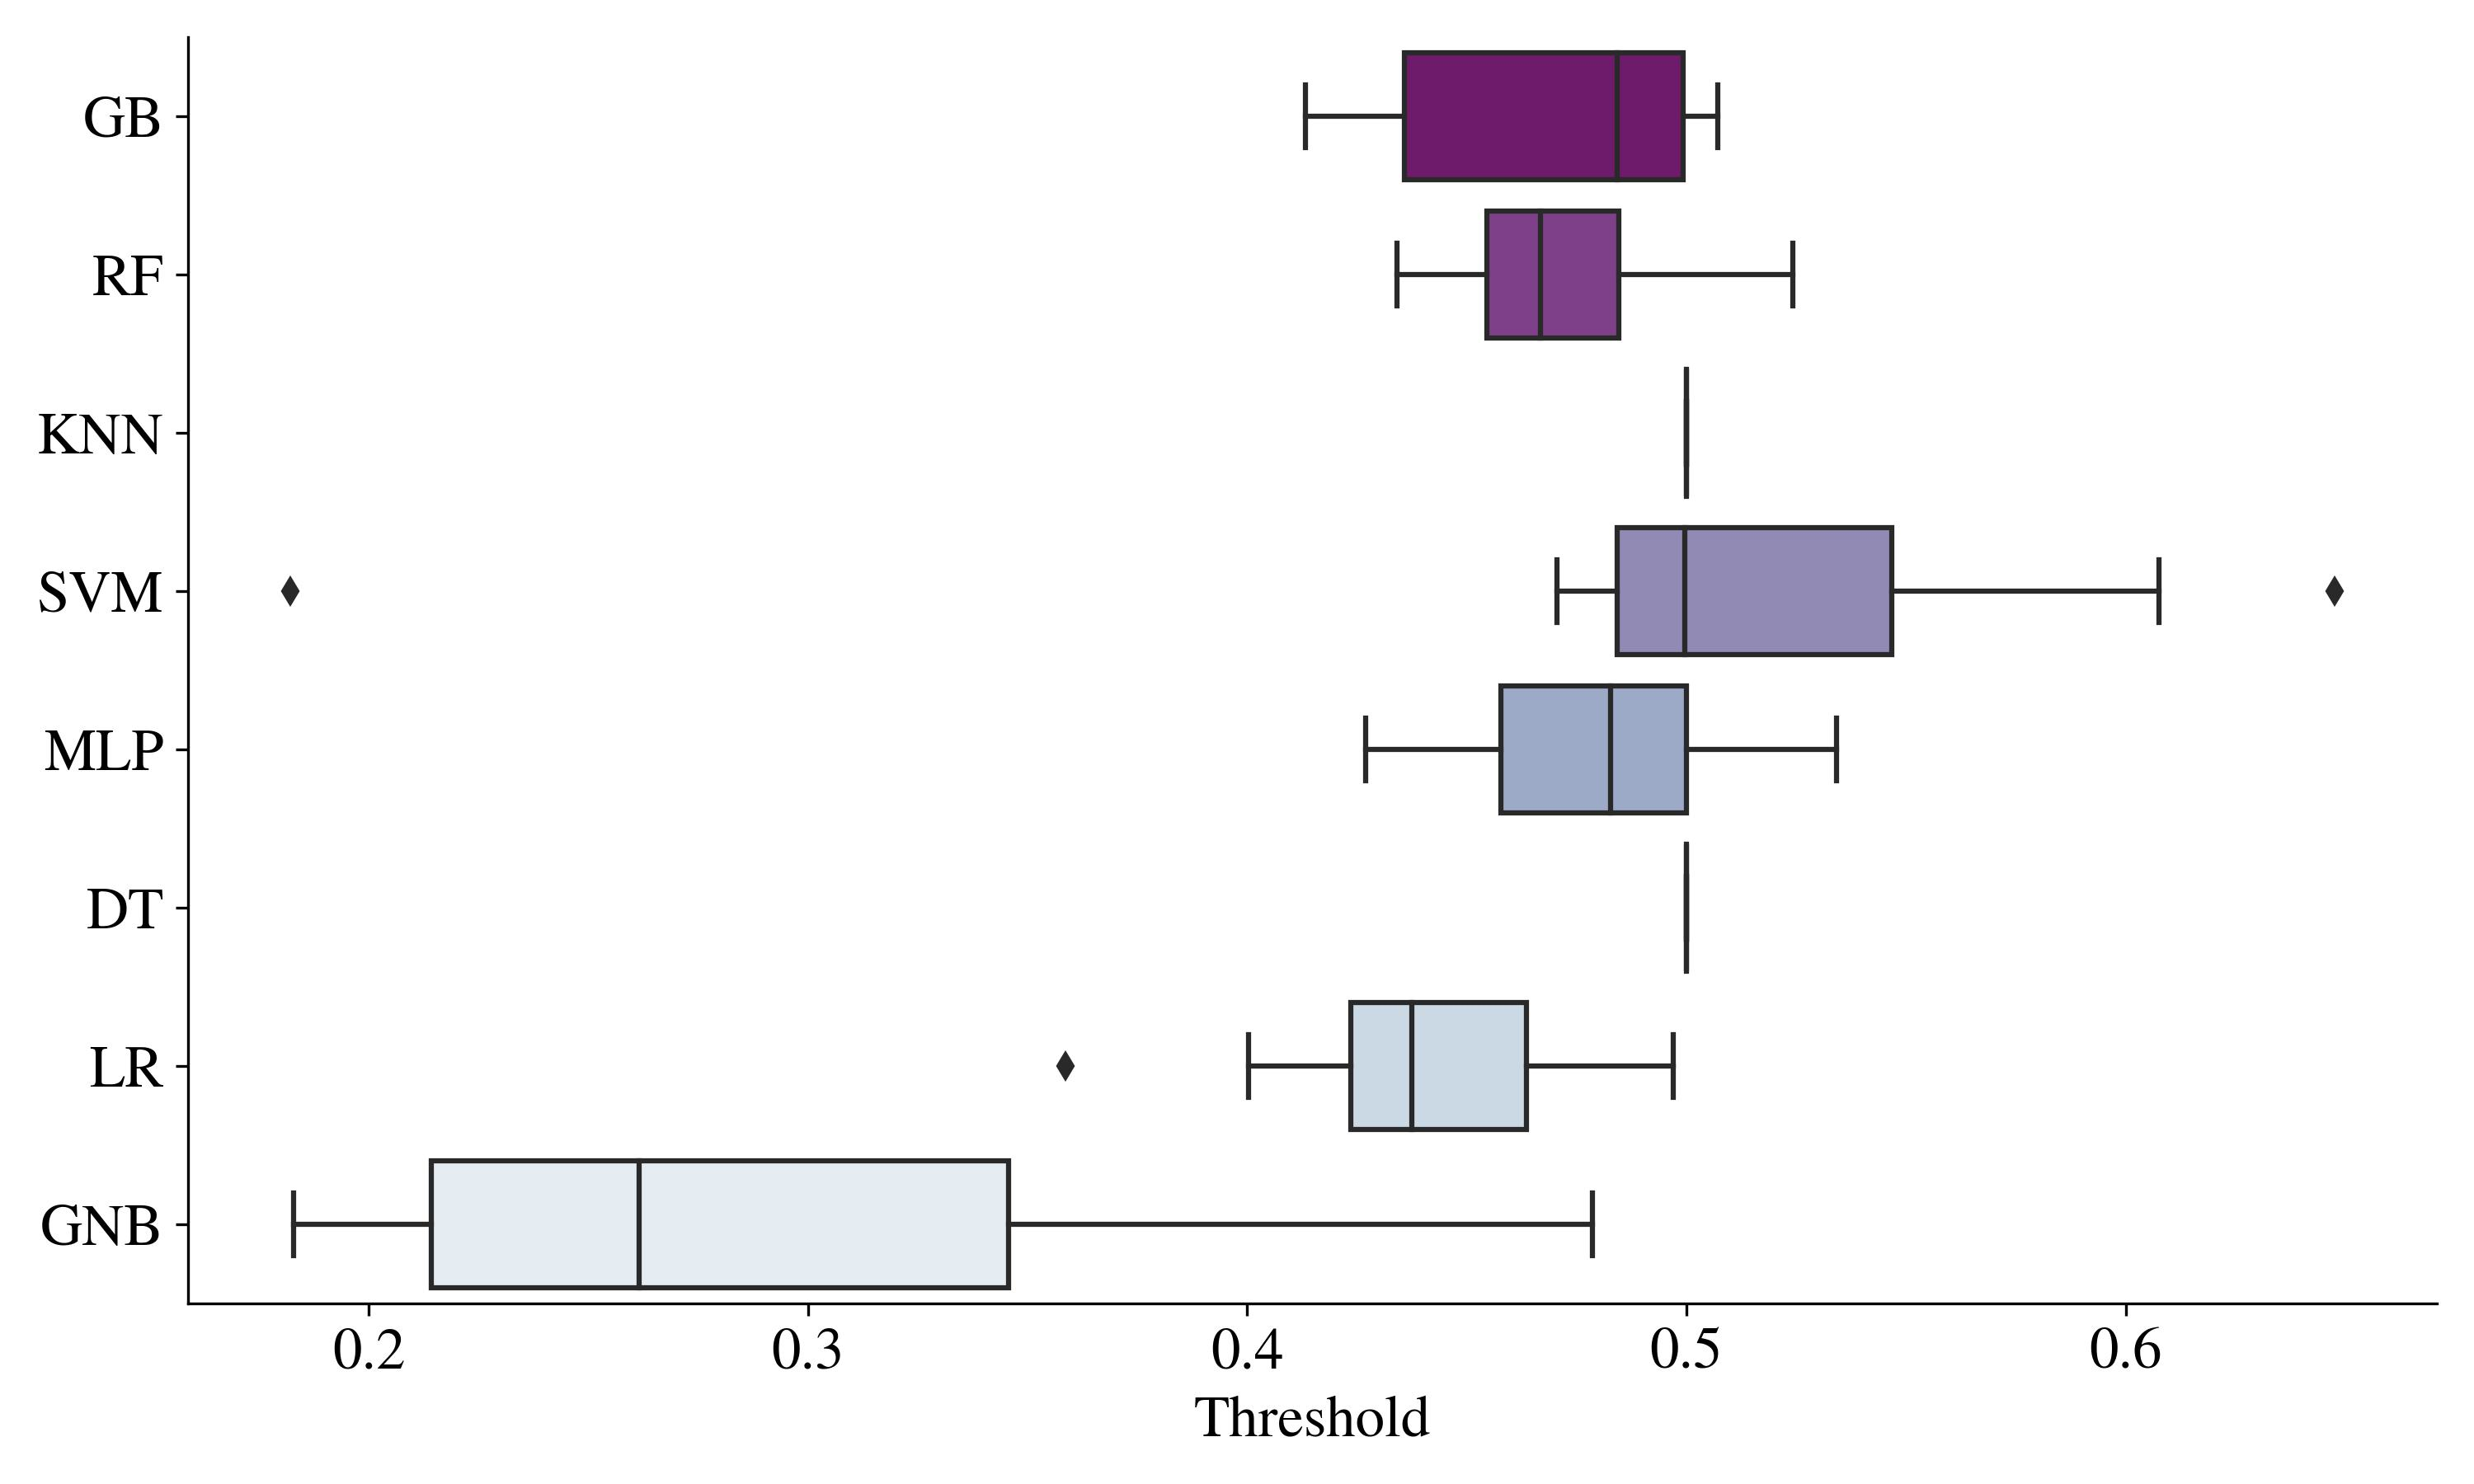
\includegraphics[width=140mm]{Figures/Threshold_wo_outliers_Distribution.jpg}

\centering{\begin{source}Author's results in Python\end{source}}\vspace{-1em}
\end{figure}

\newpage
Upon examining the execution time of each model, it can be observed that the transparent and non-complex models such as Logistic Regression, Gaussian Naive Bayes, or even Decision Tree, which take around only 1 minute to optimize themselves, also perform poorly, as already inspected in \autoref{fig:f1distclean}.
Conversely, the most time-consuming models are undoubtedly the Neural Network models, which take around 30 minutes to optimize themselves. Other time-consuming models include Gradient Boosting and Support Vector Machine, which take around 13 and 11 minutes to optimize themselves, respectively.
This finding suggests that longer execution time does not necessarily lead to better performance, as the Neural Network models are significantly outperformed by several other models.
\begin{figure}[H]
\centering
\caption{Execution Time Distribution}\vspace{0.5em}
\label{fig:timedist}\
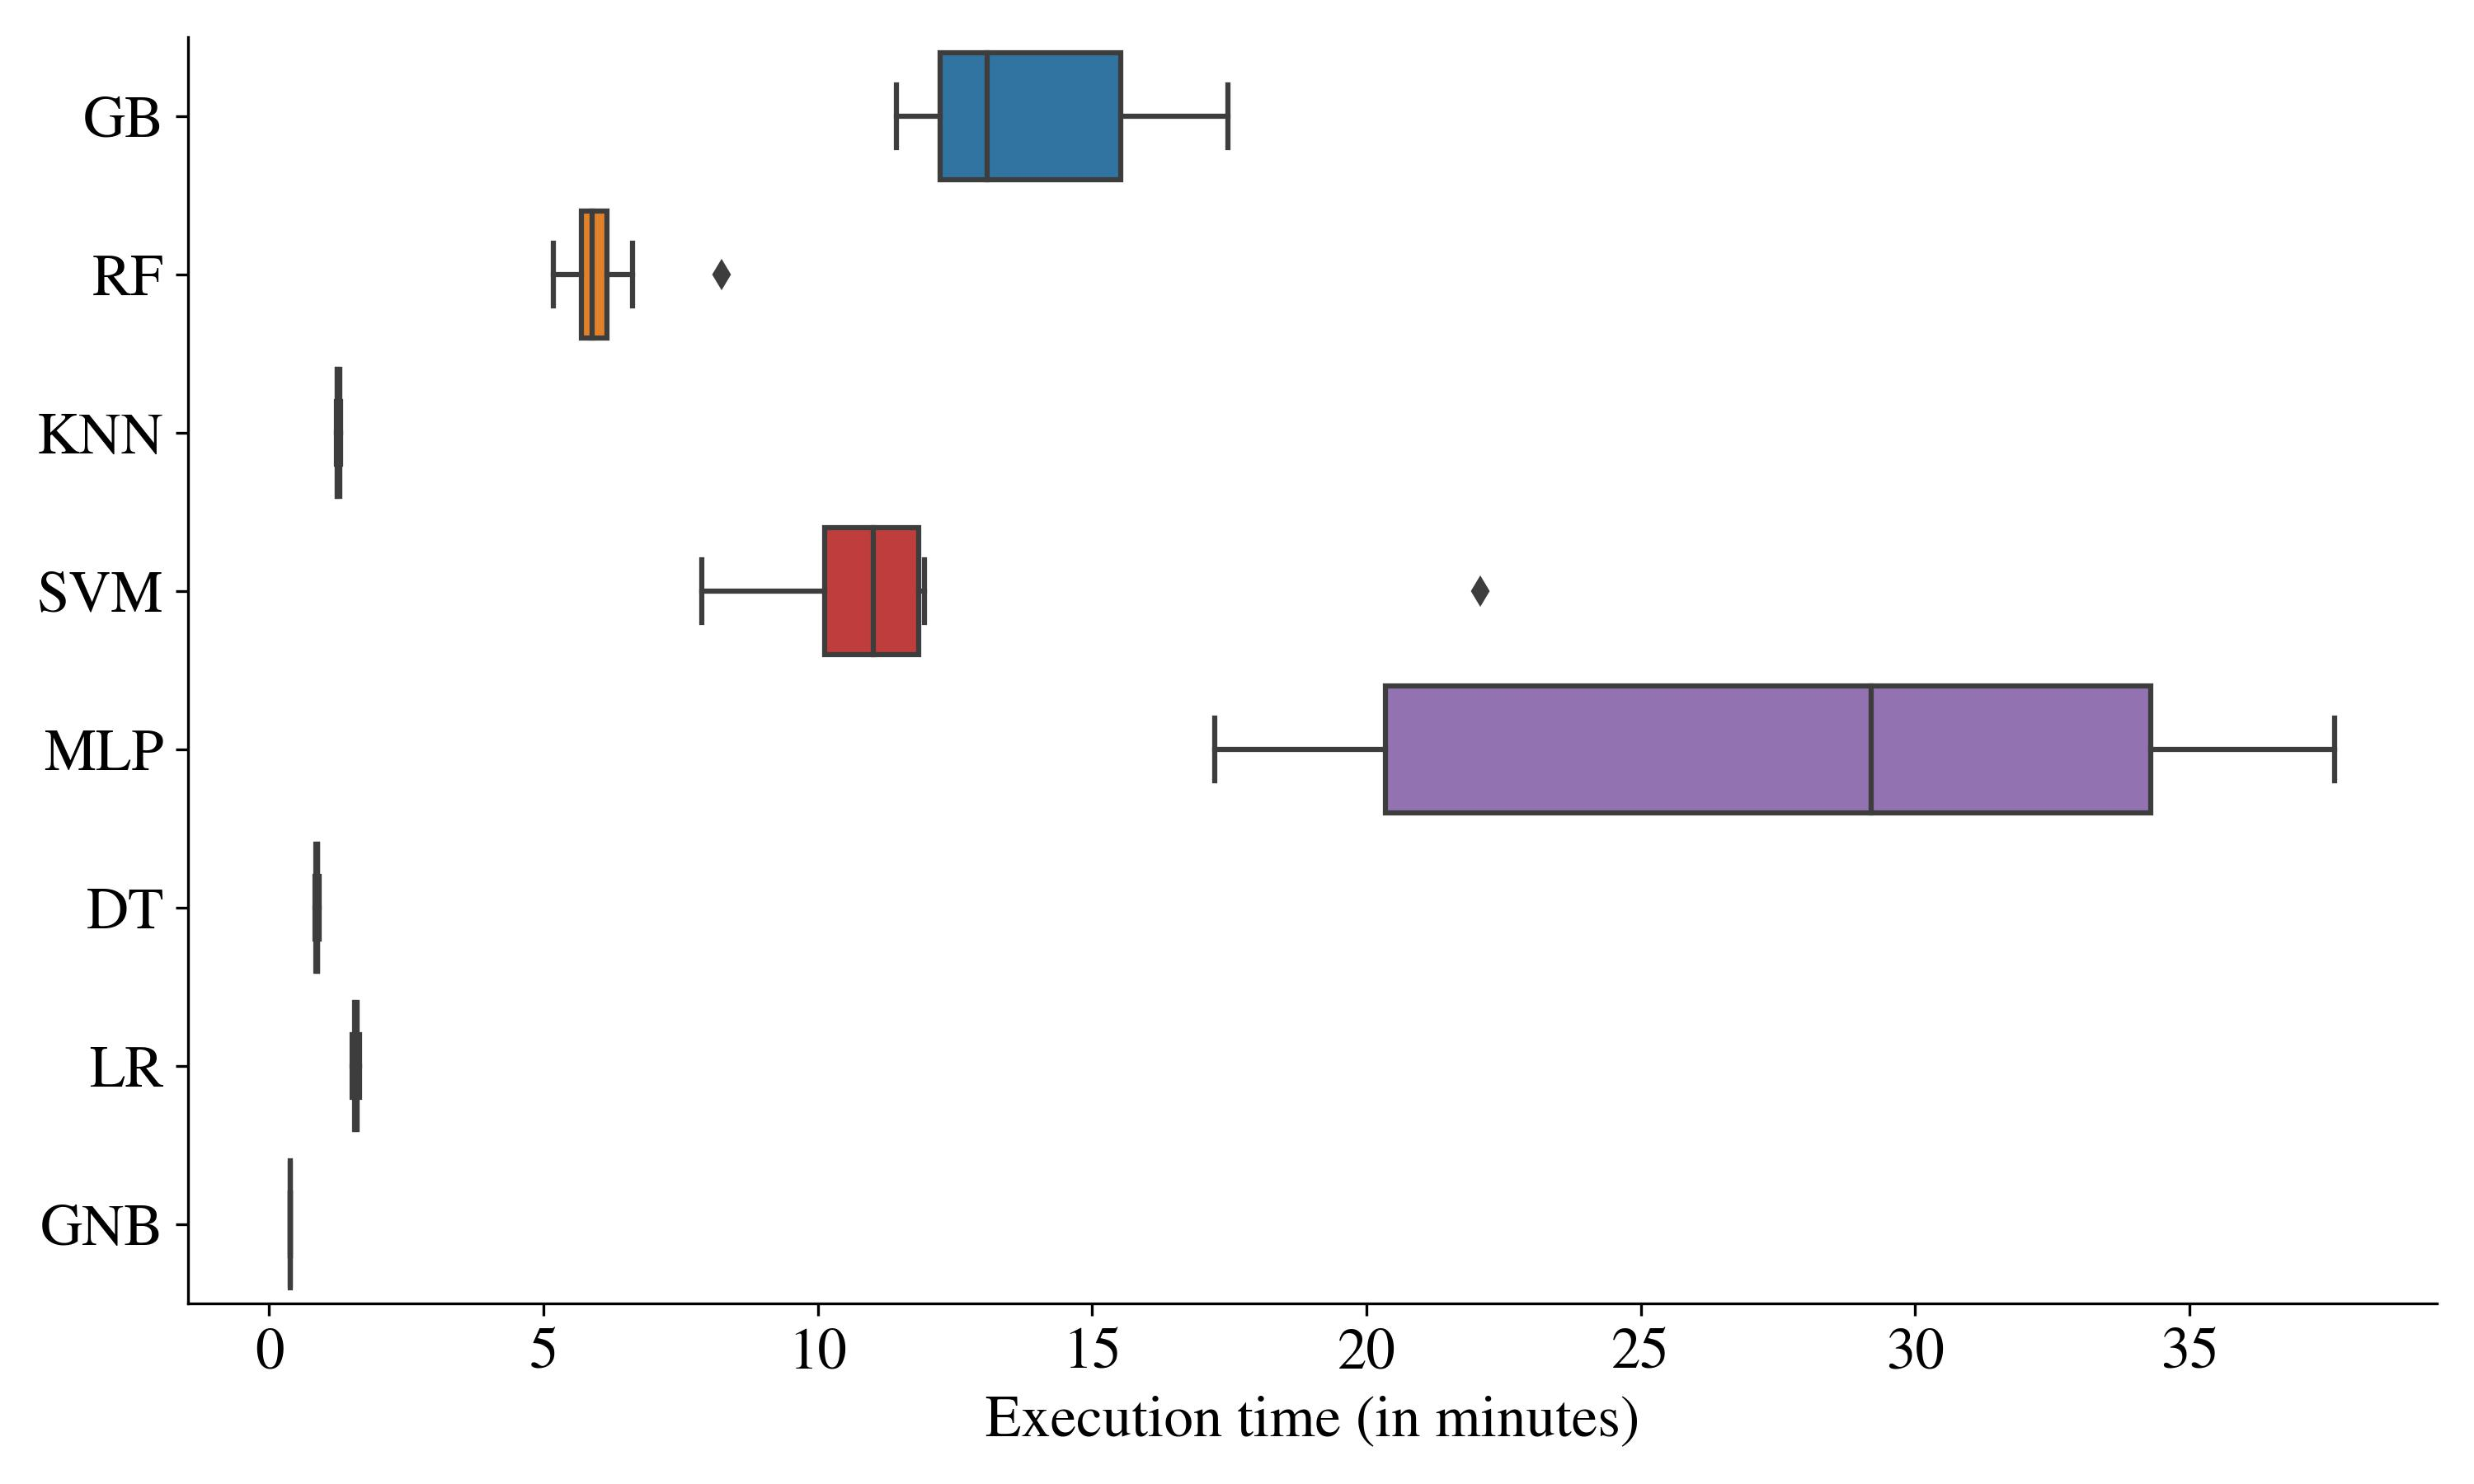
\includegraphics[width=140mm]{Figures/EXECUTION_TIME_Distribution.jpg}

\centering{\begin{source}Author's results in Python\end{source}}\vspace{-1em}
\end{figure}

\newpage
We can inspect the execution time from another perspective as shown in \autoref{fig:timedistbbwb}.
It can be observed that black--box models take a significantly longer amount of time to optimize than the white--box models, which is due to the complexity of the black--box models.
Further we can notice that some of the black--box models took only a few minutes to optimize themselves. This corresponds to KNN models, and it can be attributed to the small sample size of the data set as well as the lower data set dimensionality (i.e., low number of features) and further given the lower number of $k$ neighbors (which is constrained to 10 at most as depicted in \autoref{tab:knnspace}).
\begin{figure}[H]
    \centering
    \caption{Execution Time Distribution (Black--box/White--box dimension)}\vspace{0.5em}
    \label{fig:timedistbbwb}\
    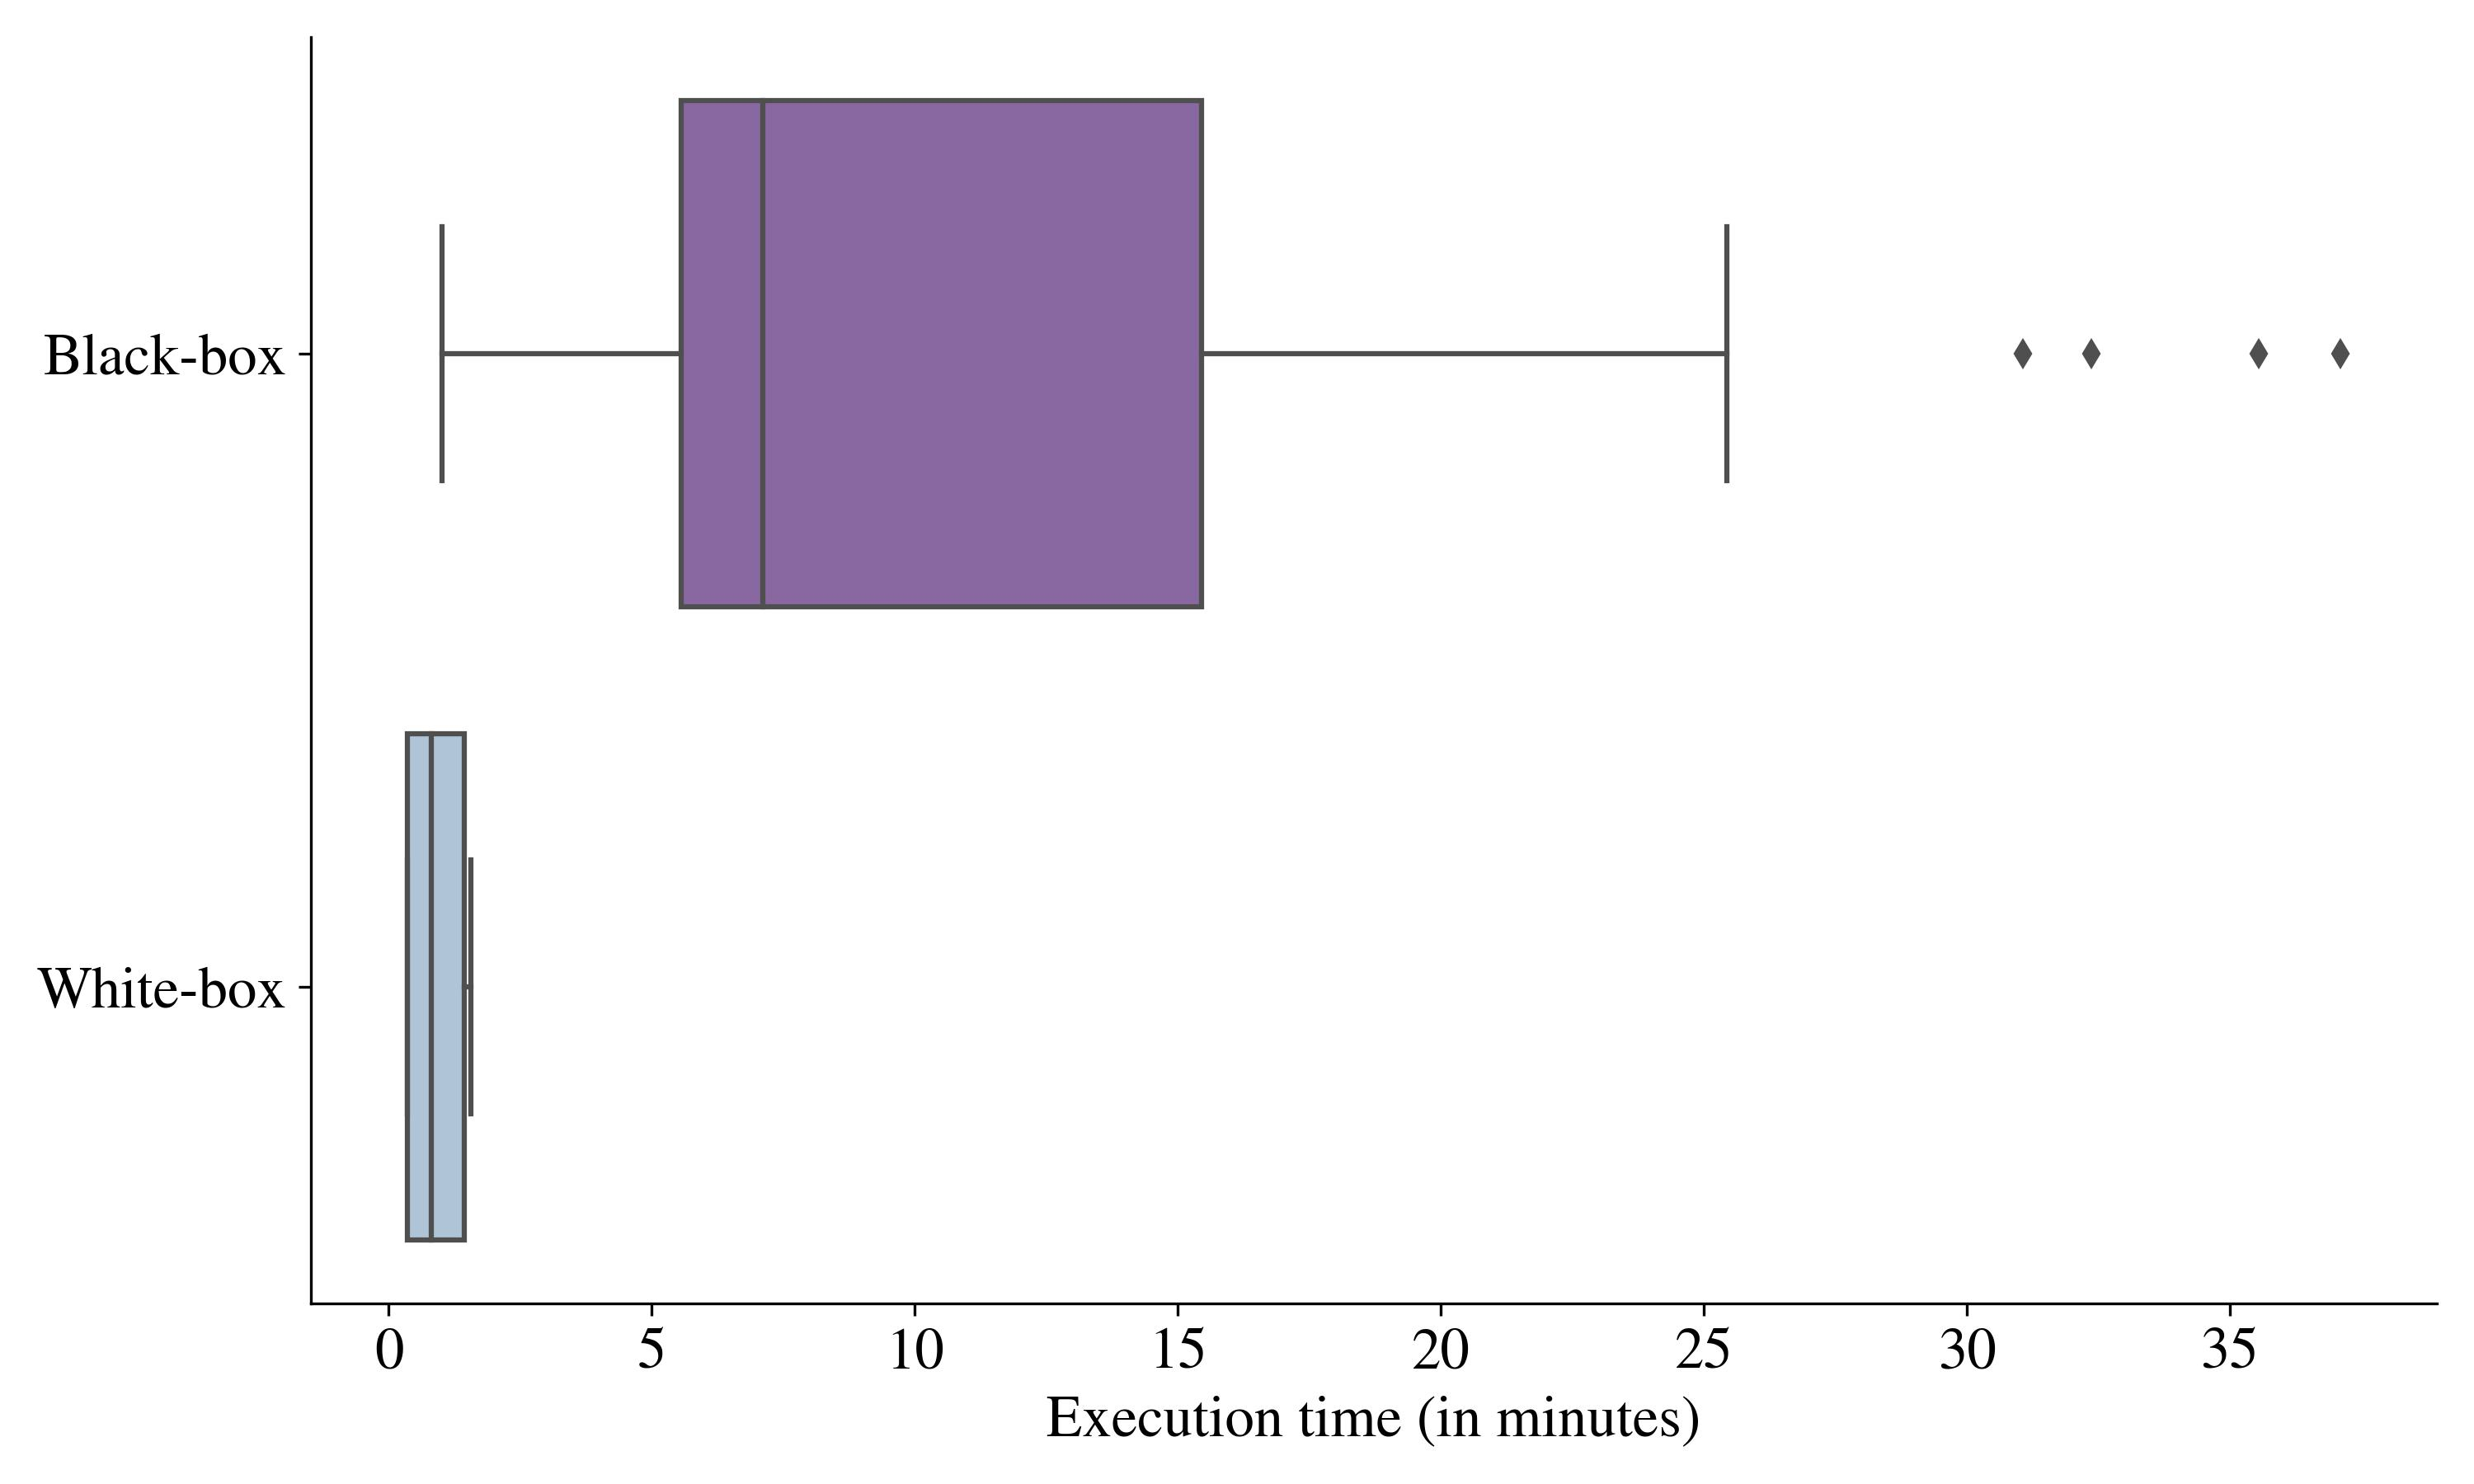
\includegraphics[width=140mm]{Figures/EXECUTION_TIME_Distribution_BB_WB.jpg}

    \centering{\begin{source}Author's results in Python\end{source}}\vspace{-1em}
\end{figure}

\newpage

The execution time and the F1 score are inspected together using a scatterplot, as shown in \autoref{fig:scattertime}. 
A cluster of non-complex and transparent models, such as Logistic Regression, Gaussian Naive Bayes, and Decision Tree, can be observed around the vertical line near 0 execution time. These models are quick to optimize, but their F1 scores are generally low.
Further, their variance in execution time is quite low, regardless of the feature subset they are optimized on.
On the other hand, the Neural Network models always perform poorly, regardless of the length of the execution time. Furthermore, the variance of the F1 scores is quite low for these models, indicating that the execution time does not have a significant impact on the F1 score in the case of Neural Networks.

\begin{figure}[H]
\centering
\caption{Execution Time vs. F1 Scatterplot - \textit{without outlier}}\vspace{0.5em}
\label{fig:scattertime}\
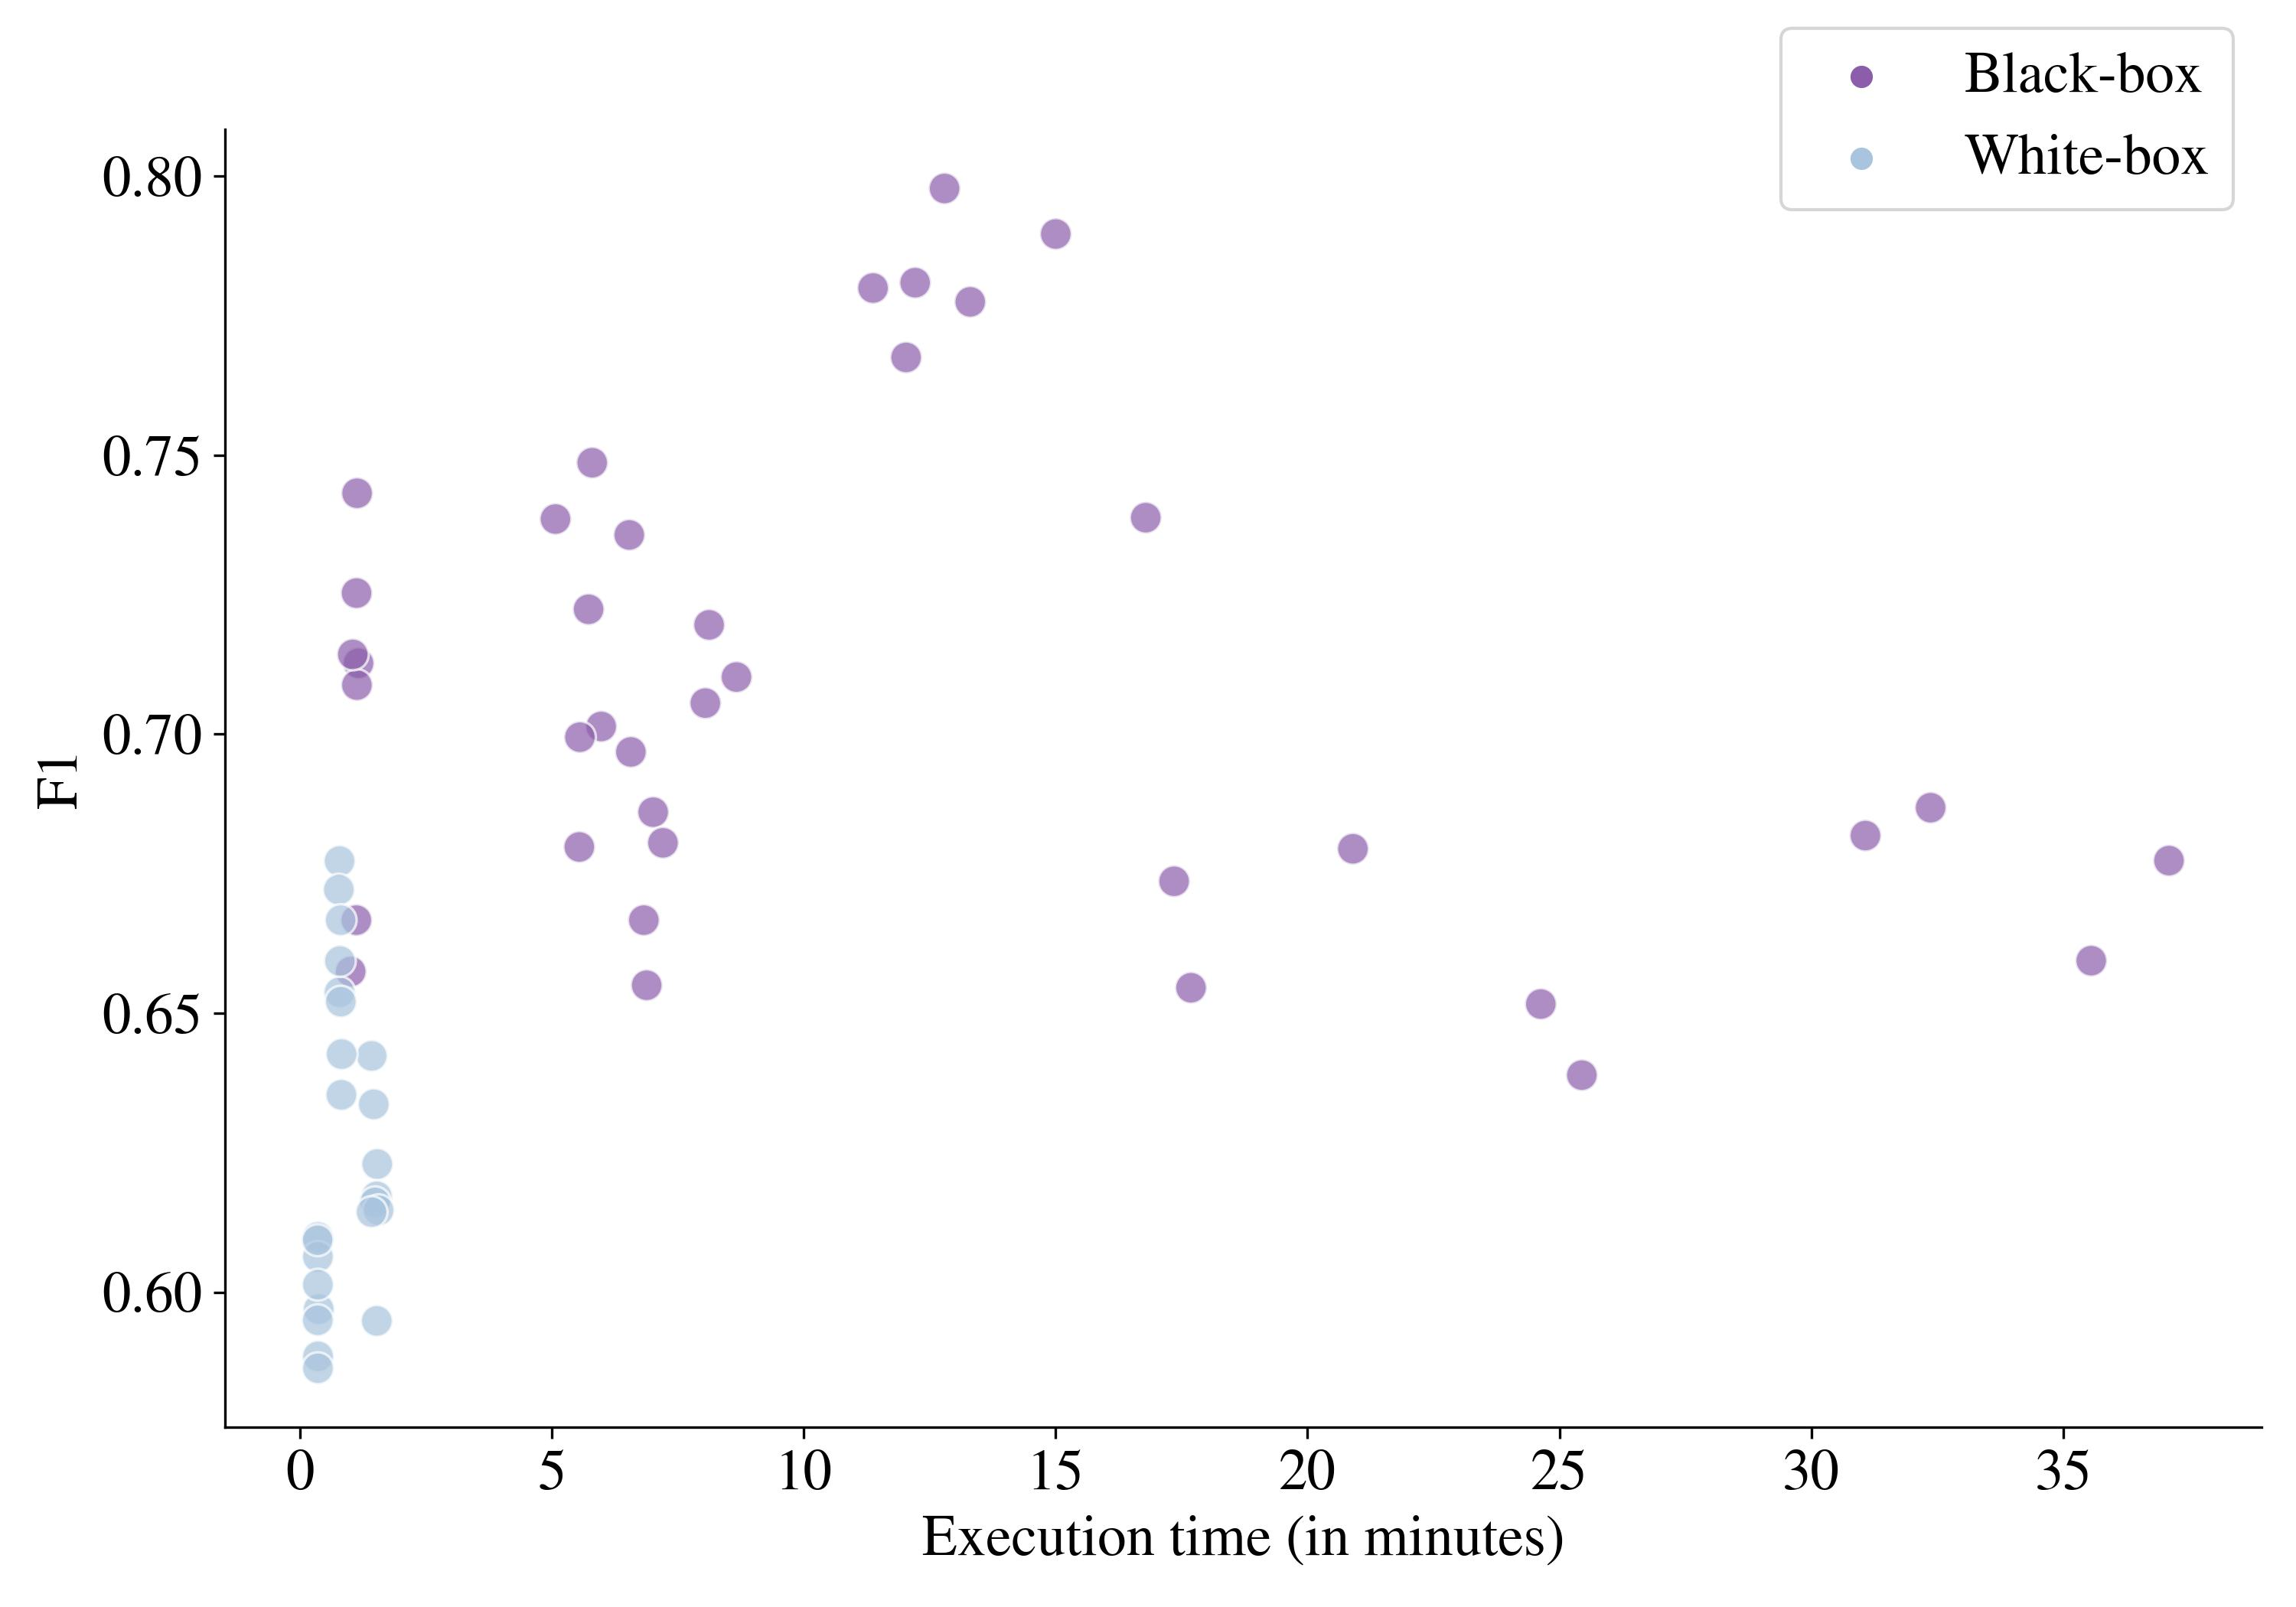
\includegraphics[width=140mm]{Figures/Scatterplot_execution_time_F1_wo_outliers.jpg}

\centering{\begin{source}Author's results in Python\end{source}}\vspace{-1em}
\end{figure}

\newpage
Such separation of the black--box and white--box models is more evident from \autoref{fig:scattertimebbwb} where the white--box models points are light blue-colored and the black--box models are purple-colored.
While the score of white--box models seems to be constant regardless of the execution time length, the points of black--box models are more dispersed across the execution time--F1 score dimension.

\begin{figure}[H]
    \centering
    \caption{Execution Time vs. F1 Scatterplot (Black--box/White--box dimension) - \textit{without outlier}}\vspace{0.5em}
    \label{fig:scattertimebbwb}\
    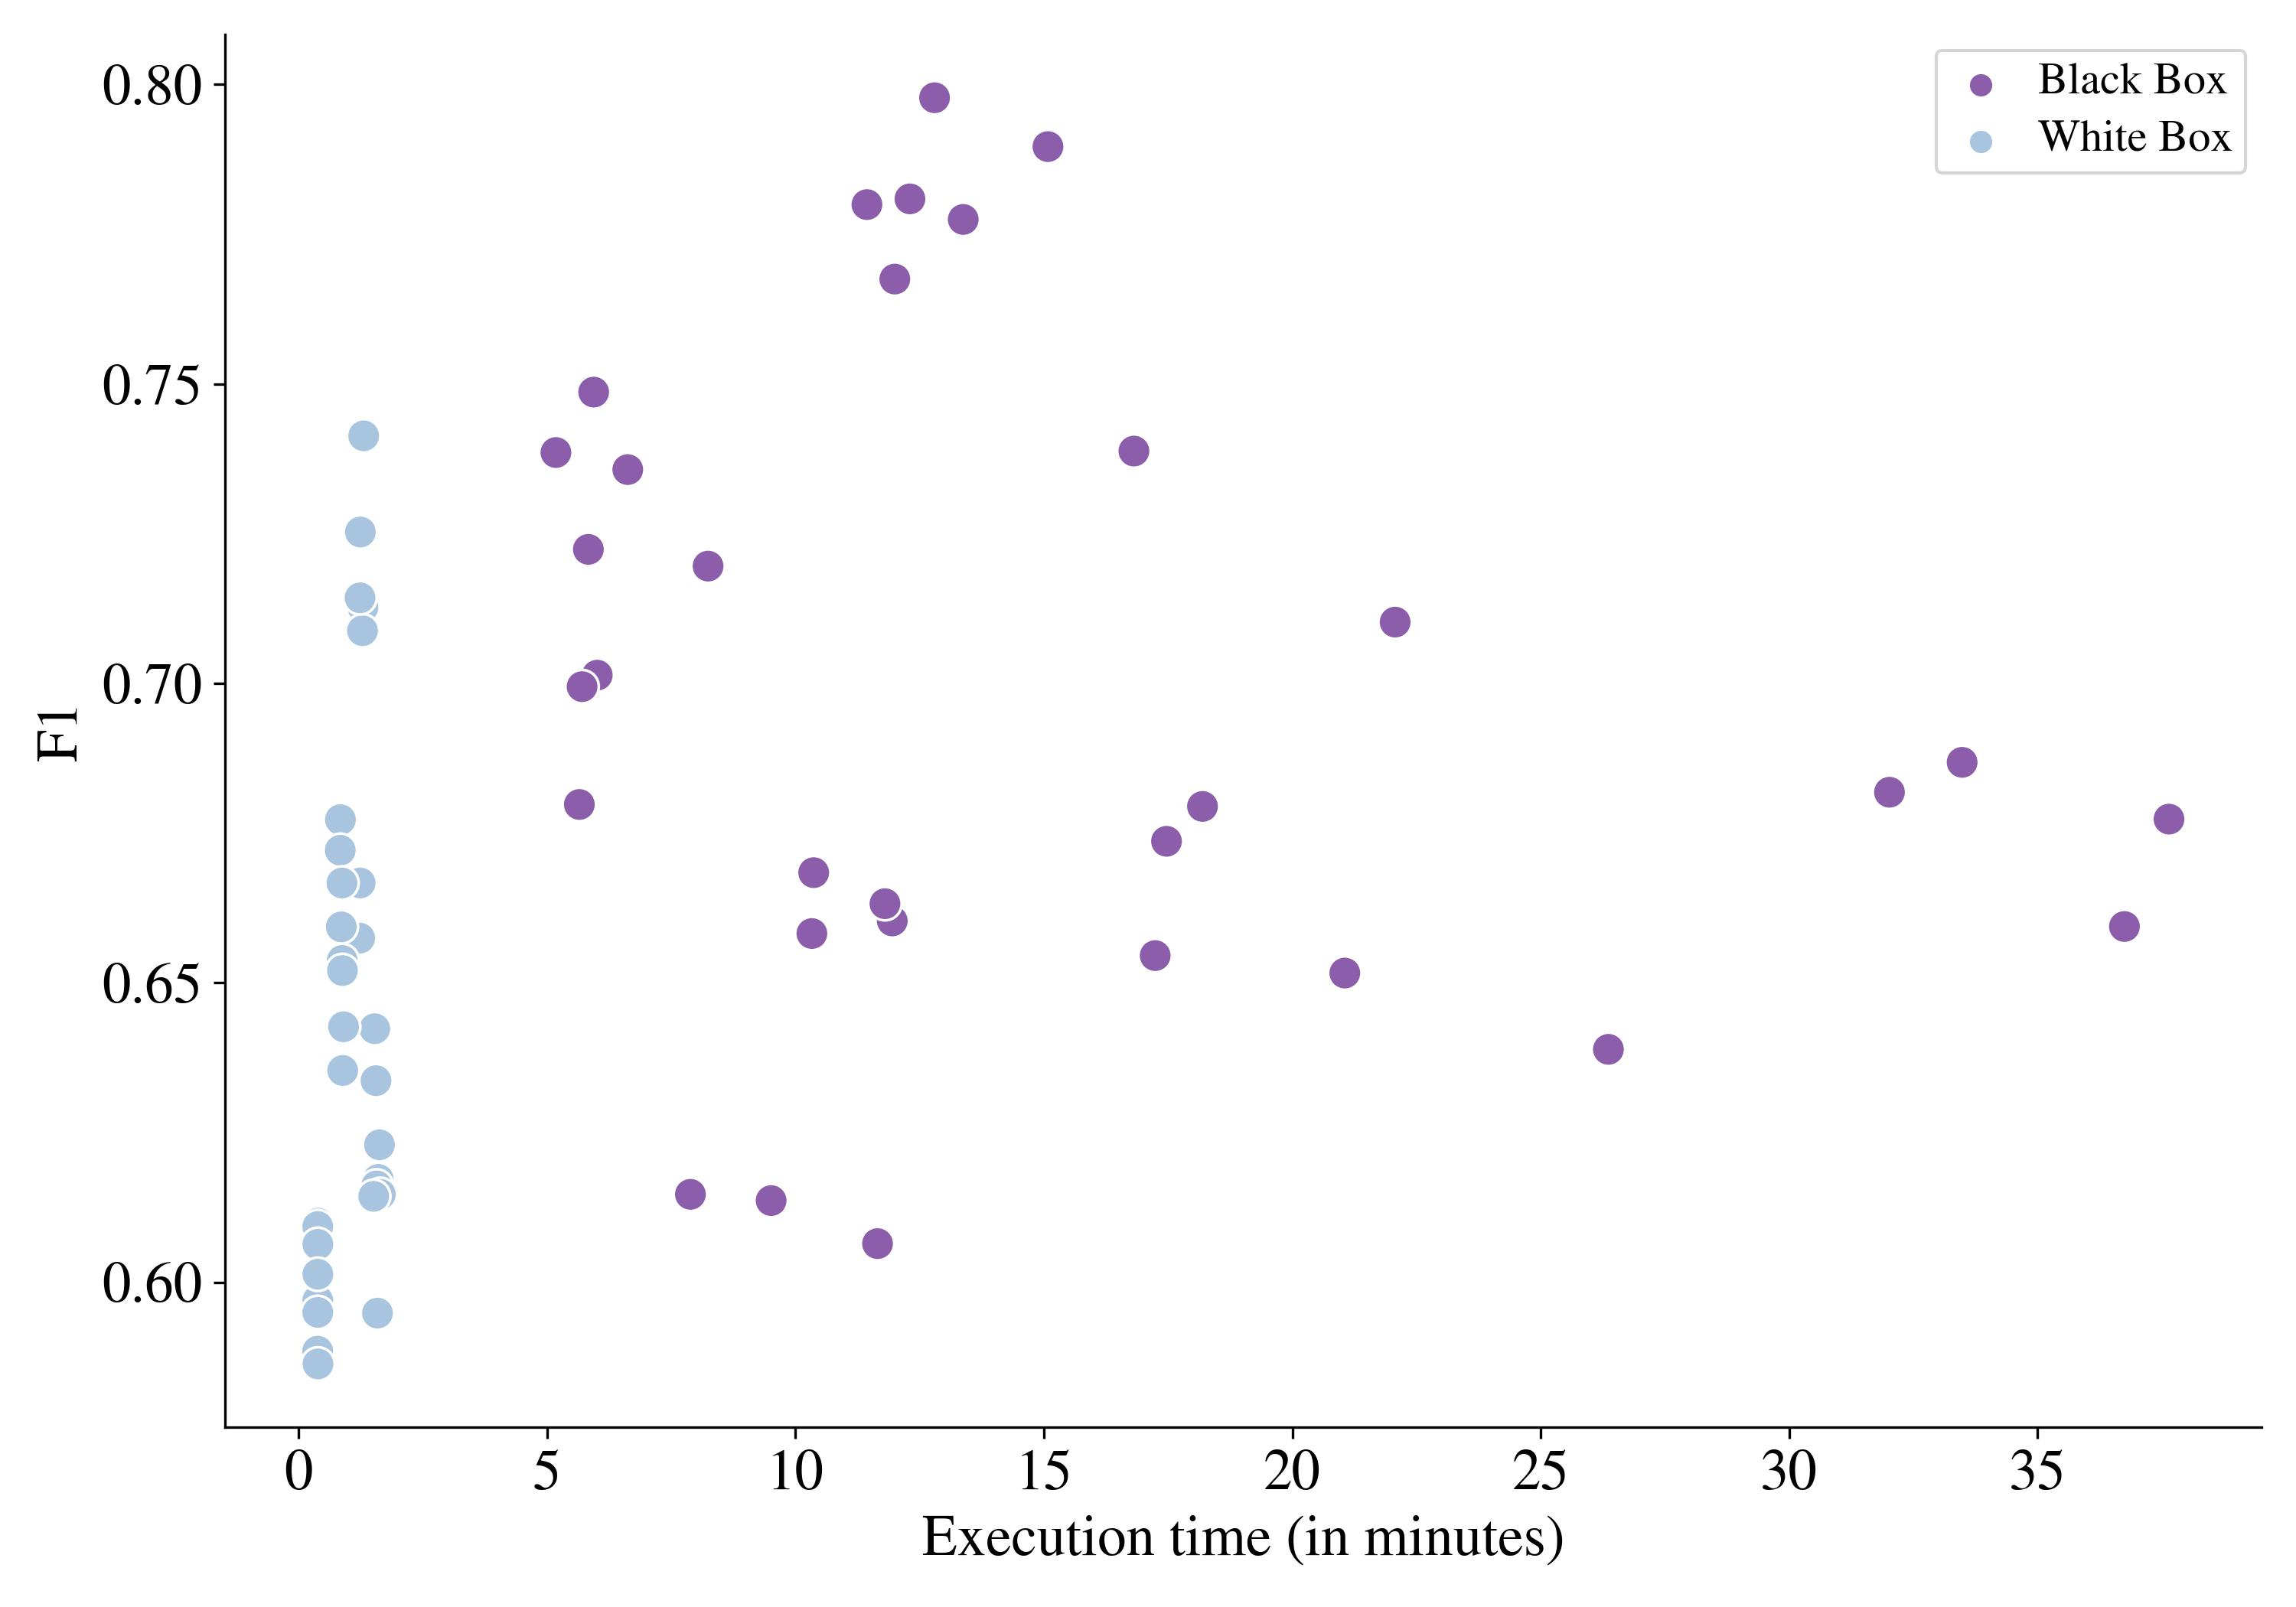
\includegraphics[width=140mm]{Figures/Scatterplot_execution_time_F1_wo_outliers_BB_WB.jpg}

    \centering{\begin{source}Author's results in Python\end{source}}\vspace{-1em}
\end{figure}

\newpage
To summarize this subsection, the best and final model is the \textbf{Gradient Boosting Classifier} which was optimized on the subset of features selected by \textbf{Multi--Layer Perceptron} - both the model information and its final hyperparameters' values are described in \autoref{tab:finalmodelinfo}. Such model is then used in the next modelling steps, including calibration, evaluation, and deployment.
\begin{table}[H]
    \small
    \setlength{\tabcolsep}{8pt}
    \renewcommand{\arraystretch}{1.3}
    \centering
    \caption{Final Model Information}\label{tab:finalmodelinfo}
    \begin{tabular}{>{\raggedleft\arraybackslash}p{0.20\linewidth}|p{0.65\linewidth}}
    \toprule
    \midrule
    \textbf{Final Model} & Gradient Boosting \\
    \midrule
    \textbf{FS Model} & Multi--Layer Perceptron \\
    \midrule
    \textbf{Final Features} &
    MORTDUE, VALUE, JOB, YOJ, DEROG, DELINQ, CLAGE, NINQ, CLNO, DEBTINC \\
    \midrule
    \textbf{Threshold} & 0.4955 \\
    \midrule
    \textbf{F1} & 0.7809 \\
    \midrule
    \textit{\# estimators} & 1,000 \\
    \midrule
    \textit{Criterion} & Friedman MSE \\
    \midrule
    \textit{Max depth} & 10 \\
    \midrule
    \textit{Max features} & 1 \\
    \midrule
    \textit{Loss} & Log loss \\
    \midrule
    \textit{Learning rate} & 0.0150 \\
    \midrule
    \bottomrule
    \end{tabular}
    \vspace{0.5em}
    
    \centering{\begin{source}Author's results in Python\end{source}}\vspace{-0.5em}
\end{table}

\newpage
\subsection{Model Recalibration}
\label{subsec:modelrecal}

In order to ensure that the final model performs well on unseen data, it is desired practice to employ the recalibration approach, which involves retraining the model on both the training and validation sets.
By doing so, the sample size used for training is increased. As such, the re-training (or so called recalibration) model leads (or is expected to lead) to a markedly improved model's performance \citep{de2023predicting}.
The recalibrated model is then used to evaluate the performance of the final model on the test set, which is the ultimate measure of a model's performance.

In addition to recalibrating the final model, it is deemed appropriate to recalibrate the threshold value for assigning class labels based on predicted probabilities. The optimal threshold value can be determined using the training and validation sets. Such threshold is recalibrated based on the training and validation sets.
In this thesis, the optimal threshold value is found to be \textbf{0.45109}, which is then used for evaluating the final model's performance on the test set.
We can observe that the model is more conservative as its optimal classification threshold has decreased. The model recalibration impact on the model's performance is further assessed in \autoref{subsec:modelperformance}.

Moreover, the recalibration process helps to mitigate overfitting issues, which occur when the model is only trained on the training set.
By incorporating the validation set into the training process, the recalibrated model can better generalize to new data and improve its overall performance on the test set.
The inclusion of the validation set during the recalibration process does not cause any data leakage issues since this set was already used during model selection to evaluate each model's performance.
Therefore, using the validation data for recalibration is a sound practice that helps to ensure the reliability and accuracy of the final model.

\newpage
\section{Model Evaluation}
\label{sec:modeleval}
After recalibrating the model and threshold, the final step in evaluating the model's performance is to test it on previously unseen data, specifically the test set.
This evaluation is critical to determining whether the model can generalize well to new data beyond the training, feature selection, and model selection phases.
During the evaluation, the recalibrated classification threshold of 0.45109 is also used.
\subsection{Model Performance Assessment}
\label{subsec:modelperformance}



In \autoref{fig:confmat}, the confusion matrix for the final model, based on the test set and using the recalibrated threshold, is presented. The matrix shows that the model is generalizing well, having correctly predicted 145 defaults and misclassified only 33 defaults, and further, correctly predicted 683 non--defaults and misclassified only 33 non--defaults. Such a result indicates that the model is a good fit for the data and can provide useful predictions.

\begin{figure}[H]
\centering
\caption{Confusion Matrix}\vspace{0.5em}
\label{fig:confmat}\
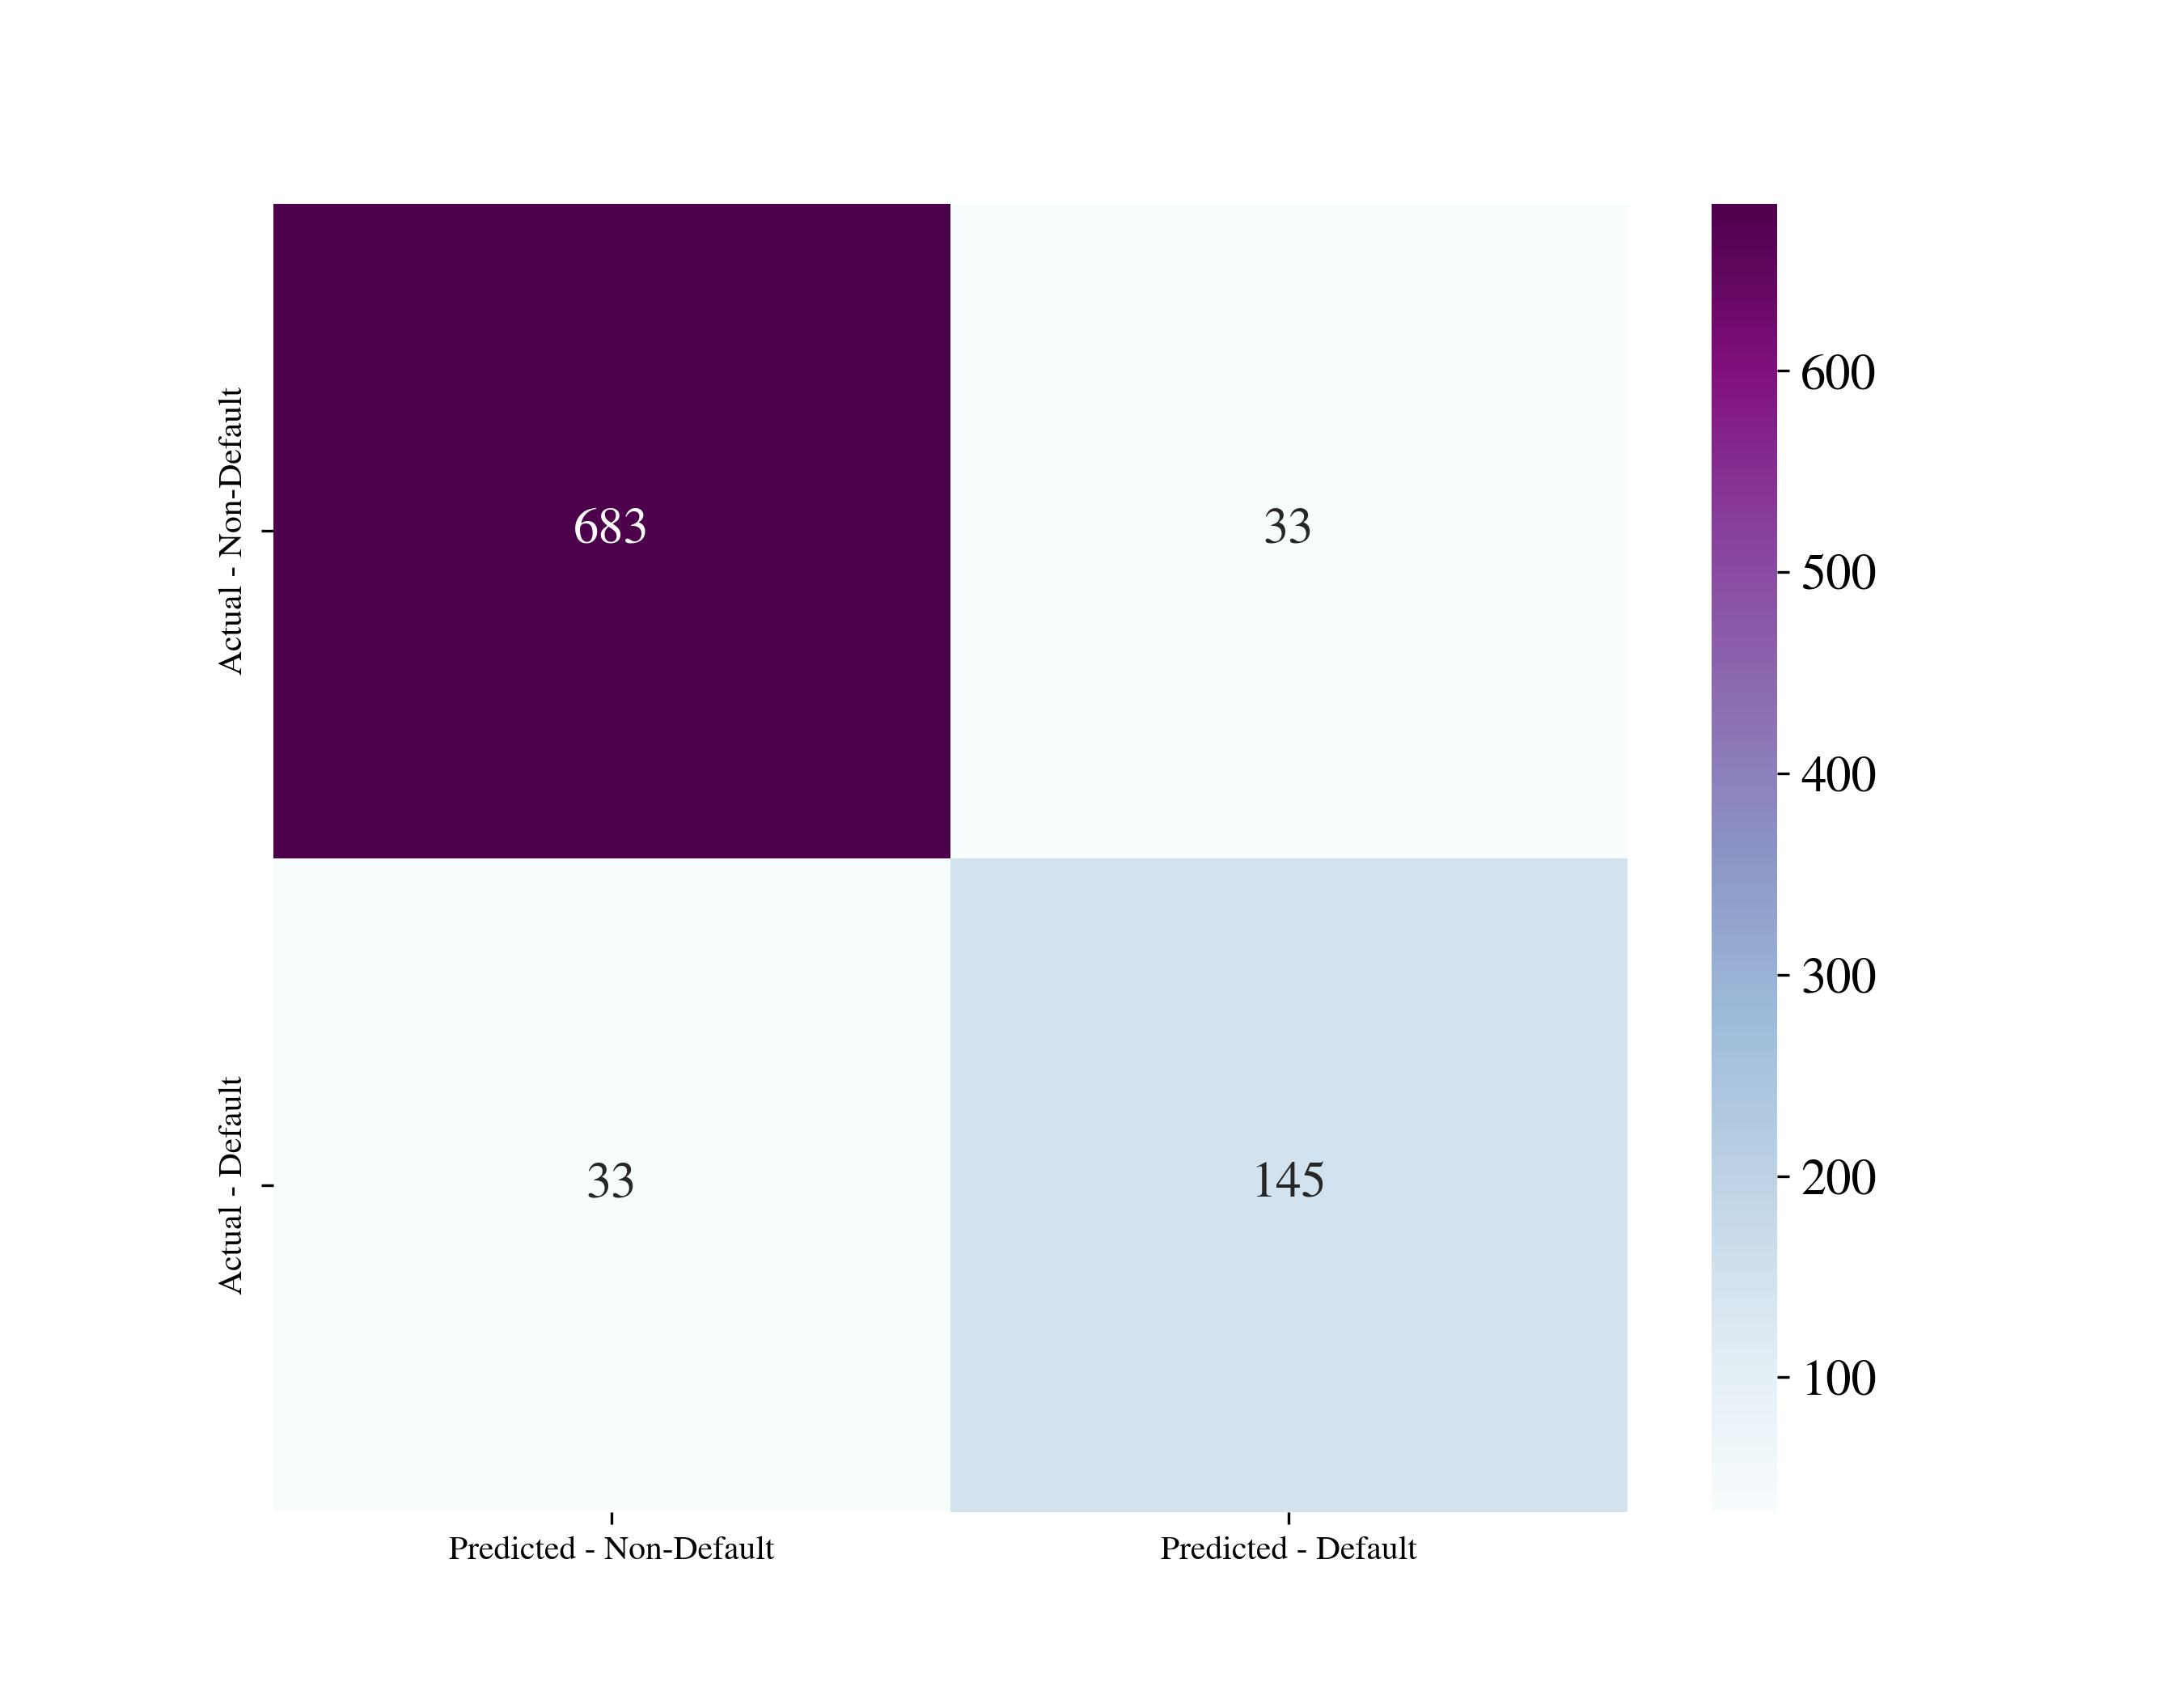
\includegraphics[width=130mm]{Figures/Confusion_Matrix.jpg}

\centering{\begin{source}Author's results in Python\end{source}}\vspace{-1em}
\end{figure}

In order to obtain a better understanding of the model's performance on previously unseen data, we computed several metrics that were used during the model selection process.
These metrics are presented in \autoref{tab:metricseval}. The results indicate that the model performs well on the unseen data, with most of the scores metrics around 80 \% to 90 \%.
Furthermore, the loss metrics are relatively low, indicating that the model can effectively distinguish between defaults and non-defaults.
Particularly, out of all test instances, the model predicts correctly 92.62 \% default instances. The model also predicts 81.46 \% instances out of all the actual default instances. Moreover, out of all predicted default instances, the model correctly predicts 81.46 \% actual default instances.
Overall, these results suggest that the model is performing well and is suitable for predicting defaults.
The results suggest that the model has a good balance between correctly identifying defaults and non-defaults, as well as minimizing False Positives and False Negatives. This further confirms the model's ability to accurately predict defaults.

\begin{table}[H]
    \small
    \setlength{\tabcolsep}{8pt}
    \renewcommand{\arraystretch}{1.3}
    \centering
        \caption[Metrics Evaluation]{Metrics Evaluation}\label{tab:metricseval}
        \begin{tabular}{@{} r r @{\hspace{1cm}} l @{}}
    \toprule
    \textbf{Metric} & \textbf{Value}\\
    \midrule
    \hline
    F1 & 0.8146 \\ 
    Precision & 0.8146 \\ 
    Recall & 0.8146 \\ 
    Accuracy & 0.9262 \\ 
    AUC & 0.9564 \\ 
    Somers' D & 0.9128 \\ 
    KS & 0.7915 \\ 
    MCC & 0.7685 \\ 
    Brier Score Loss & 0.0594 \\
    Log Loss & 0.2163 \\
    \hline
    \bottomrule
    \end{tabular}
    \vspace{0.35em}

        \centering{\begin{source}Author's results in Python\end{source}}\vspace{-1em}
\end{table}

The following \autoref{tab:recab} shows the impact of recalibration on the model's performance metrics. $M_{NR}$ denotes the final model that was not recalibrated at all (i.e., trained only on the training set), whereas $M_R$ denotes the recalibrated model (i.e., trained on the joined training and validation sets). Respectively, $M_{NR}$ uses its threshold computed based on the training set (0.4955), and $M_R$ uses its threshold computed on the joined training and validation set(0.45109).
As can be seen, the recalibration indeed has a positive impact on the metrics evaluation, as all the metric scores have increased, while the metric loss functions have decreased.
We can observe the most significant decrease in the Log Loss function, which has decreased by 8.09 \%, while the objective function F1 score has increased by 3.30 \% thanks to increases in both Precision and Recall.
Therefore, the recalibration process is deemed desirable and appropriate in terms of the model's performance.


\begin{table}[H]
    \small
    \setlength{\tabcolsep}{8pt}
    \renewcommand{\arraystretch}{1.3}
    \centering
        \caption[Recalibration Impact on Metrics Evaluation]{Recalibration Impact on Metrics Evaluation}\label{tab:recab}
        \begin{tabular}{@{} r r @{\hspace{0.5cm}} r @{\hspace{0.5cm}} r @{}}
            \toprule
            \textbf{Metric} & \textbf{$M_{NR}$} & \textbf{$M_{R}$} & \textbf{Diff.}\\
    \midrule
    \hline
    F1 & 0.7886 & 0.8146 & 3.30 \% \\ 
    Precision & 0.8023 & 0.8146 & 1.53 \% \\ 
    Recall & 0.7753 & 0.8146 & 5.07 \% \\ 
    Accuracy & 0.9172 & 0.9262 & 0.98 \% \\ 
    AUC & 0.9518 & 0.9564  & 0.48 \% \\ 
    Somers' D & 0.9037 & 0.9128 & 1.01 \% \\ 
    KS & 0.7845 & 0.7915 & 0.89 \% \\ 
    MCC & 0.7373 & 0.7685 & 4.23 \% \\ 
    Brier Score Loss & 0.0632 & 0.0594 & -6.11 \% \\
    Log Loss & 0.2353 & 0.2163 & -8.09 \% \\
    \hline
    \bottomrule
    \end{tabular}
    \vspace{0.35em}

        \centering{\begin{source}Author's results in Python\end{source}}\vspace{-1em}
\end{table}

To further evaluate the performance of the recalibrated final model, we can visualize the ROC curve, as presented in \autoref{fig:roc}. The curve illustrates the trade-off between the True Positive Rate and the False Positive Rate at various classification thresholds. An ideal ROC curve should have an Area Under the Curve (AUC) value of 100 \%, indicating a perfect classifier, while a random classifier would have an AUC of 50 \%.

From the ROC curve plot, we observe that the AUC value of the model is 95.64 \%, indicating a high degree of accuracy in distinguishing between defaults and non-defaults. The curve covers most of the area above the diagonal line, indicating that the model is performing well in differentiating the two classes. Therefore, the results suggest that the model is performing well and is capable of accurately identifying potential defaulters.

\begin{figure}[H]
\centering
\caption{ROC Curve}\vspace{0.5em}
\label{fig:roc}\
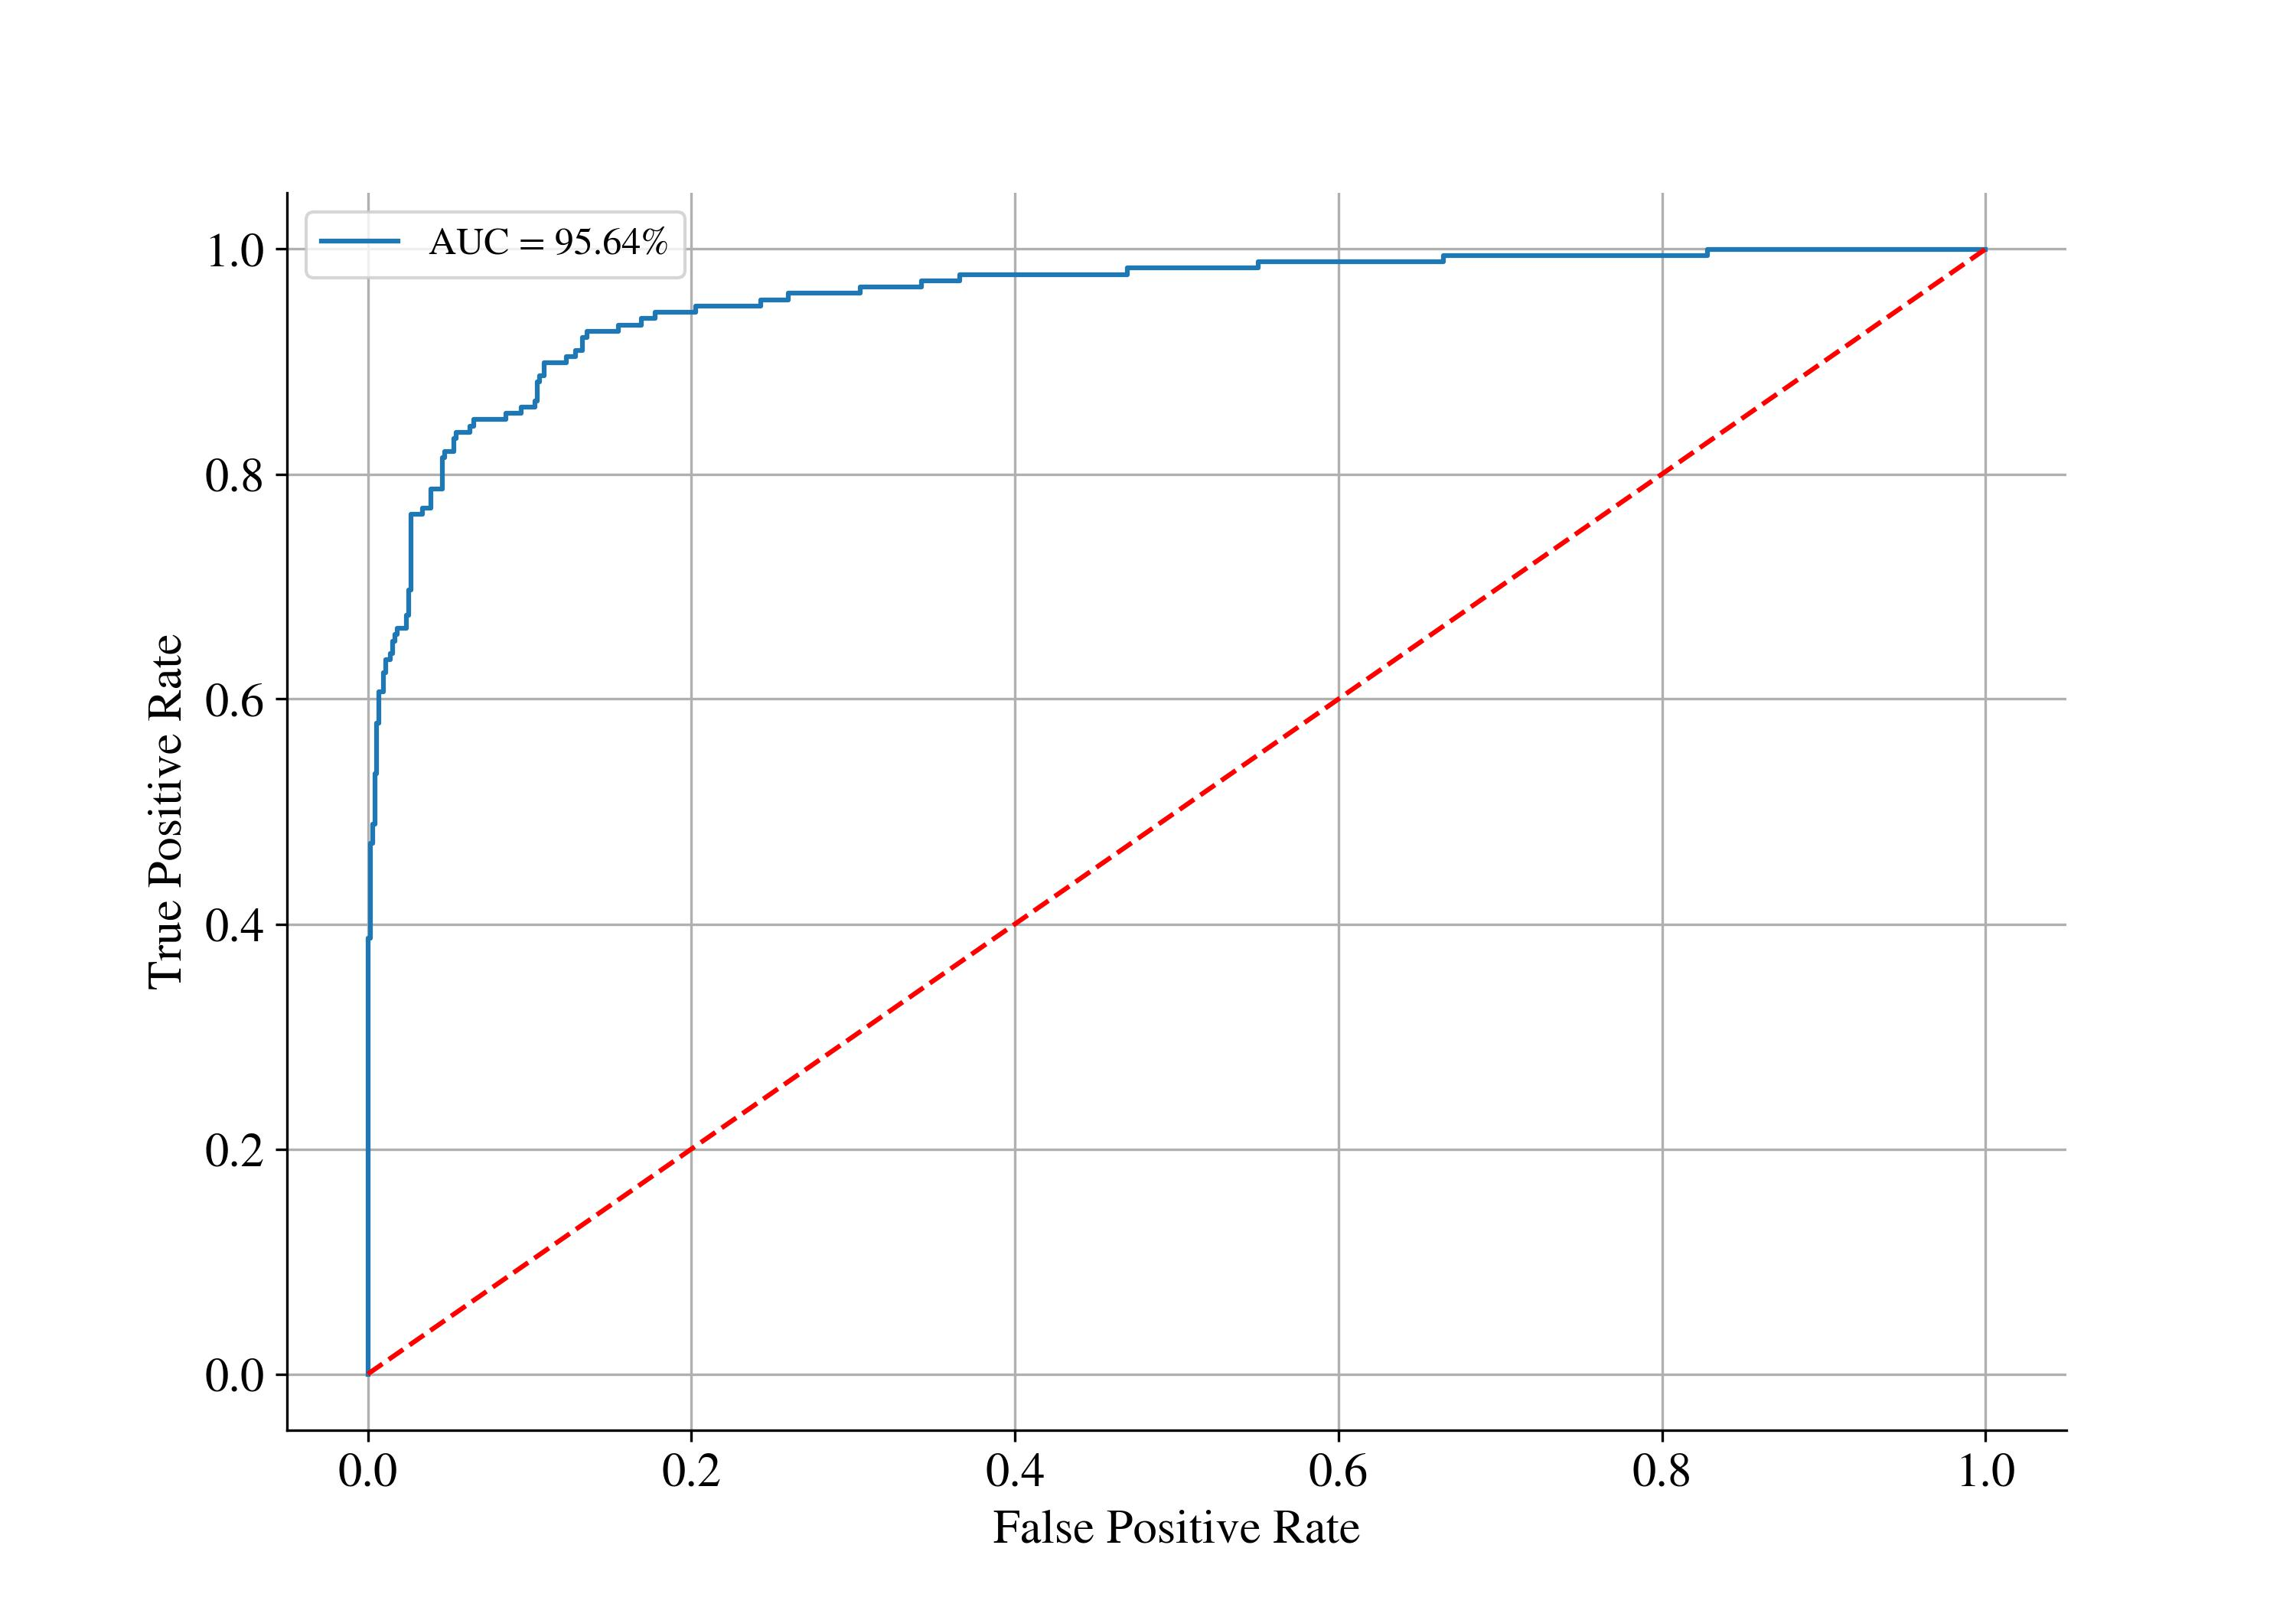
\includegraphics[width=140mm]{Figures/ROC_curve_FINAL.jpg}

\centering{\begin{source}Author's results in Python\end{source}}\vspace{-1em}
\end{figure}



\subsection{Model Explainability}
\label{subsec:explainability}

To gain insights into the impact of the features used in the final model, we can inspect the feature importances of the final model, which is a part of a family of tree ensemble algorithms.
As the name indicates, it is the score value representing the importance of the features, i.e., the higher the score, the more important the feature is. Basically, it is a measure of how much a feature contributes to the overall performance of the model.
Overall, the feature importance plot provides valuable insights into the factors that are most important in predicting loan defaults. It can be used to identify which features are contributing the most to the model's accuracy and to guide future feature selection efforts.
According to Bonaccorso \citep{bonaccorso2020mastering}, feature importance is the measure proportional to the impurity reduction that a particular feature allows us to achieve, and is defined as:
\begin{equation}\label{eq}
    \text{FI}\left(\bar{x}^{\left(i\right)}\right) = \frac{1}{N} \displaystyle\sum_{k=1}^{N} \displaystyle\sum_{j=1}^{L} \frac{n(j)}{M} \delta I_{j}^{i}
\end{equation}
where $ \text{FI}\left(\bar{x}^{\left(i\right)}\right)$ refers to the feature importance of the feature $i$, $n(j)$ is the number of samples reaching the node $j$, $\delta I_{j}^{i}$ represents the impurity reduction at node $j$ after the splitting using the feature $j$, $M$ is total number of samples in the data set used to built the model, and $N$ refers to the number of tree estimators used within an ensemble model.

The following \autoref{fig:fi} depicts the feature importances of all the selected features on which the final model was trained.
The two most important features used in the final model are \texttt{DEBTINC} and \texttt{DELINQ}, which are crucial debt and delinquency indicators in determining whether a borrower would be able to repay their loan. These two features have a significant impact on the model's ability to accurately predict loan defaults, with high feature importance scores. This is also in line with the findings from the exploratory analysis, WoE distribution, or feature selection.
\begin{figure}[H]
\centering
\caption{Feature Importance}\vspace{0.5em}
\label{fig:fi}\
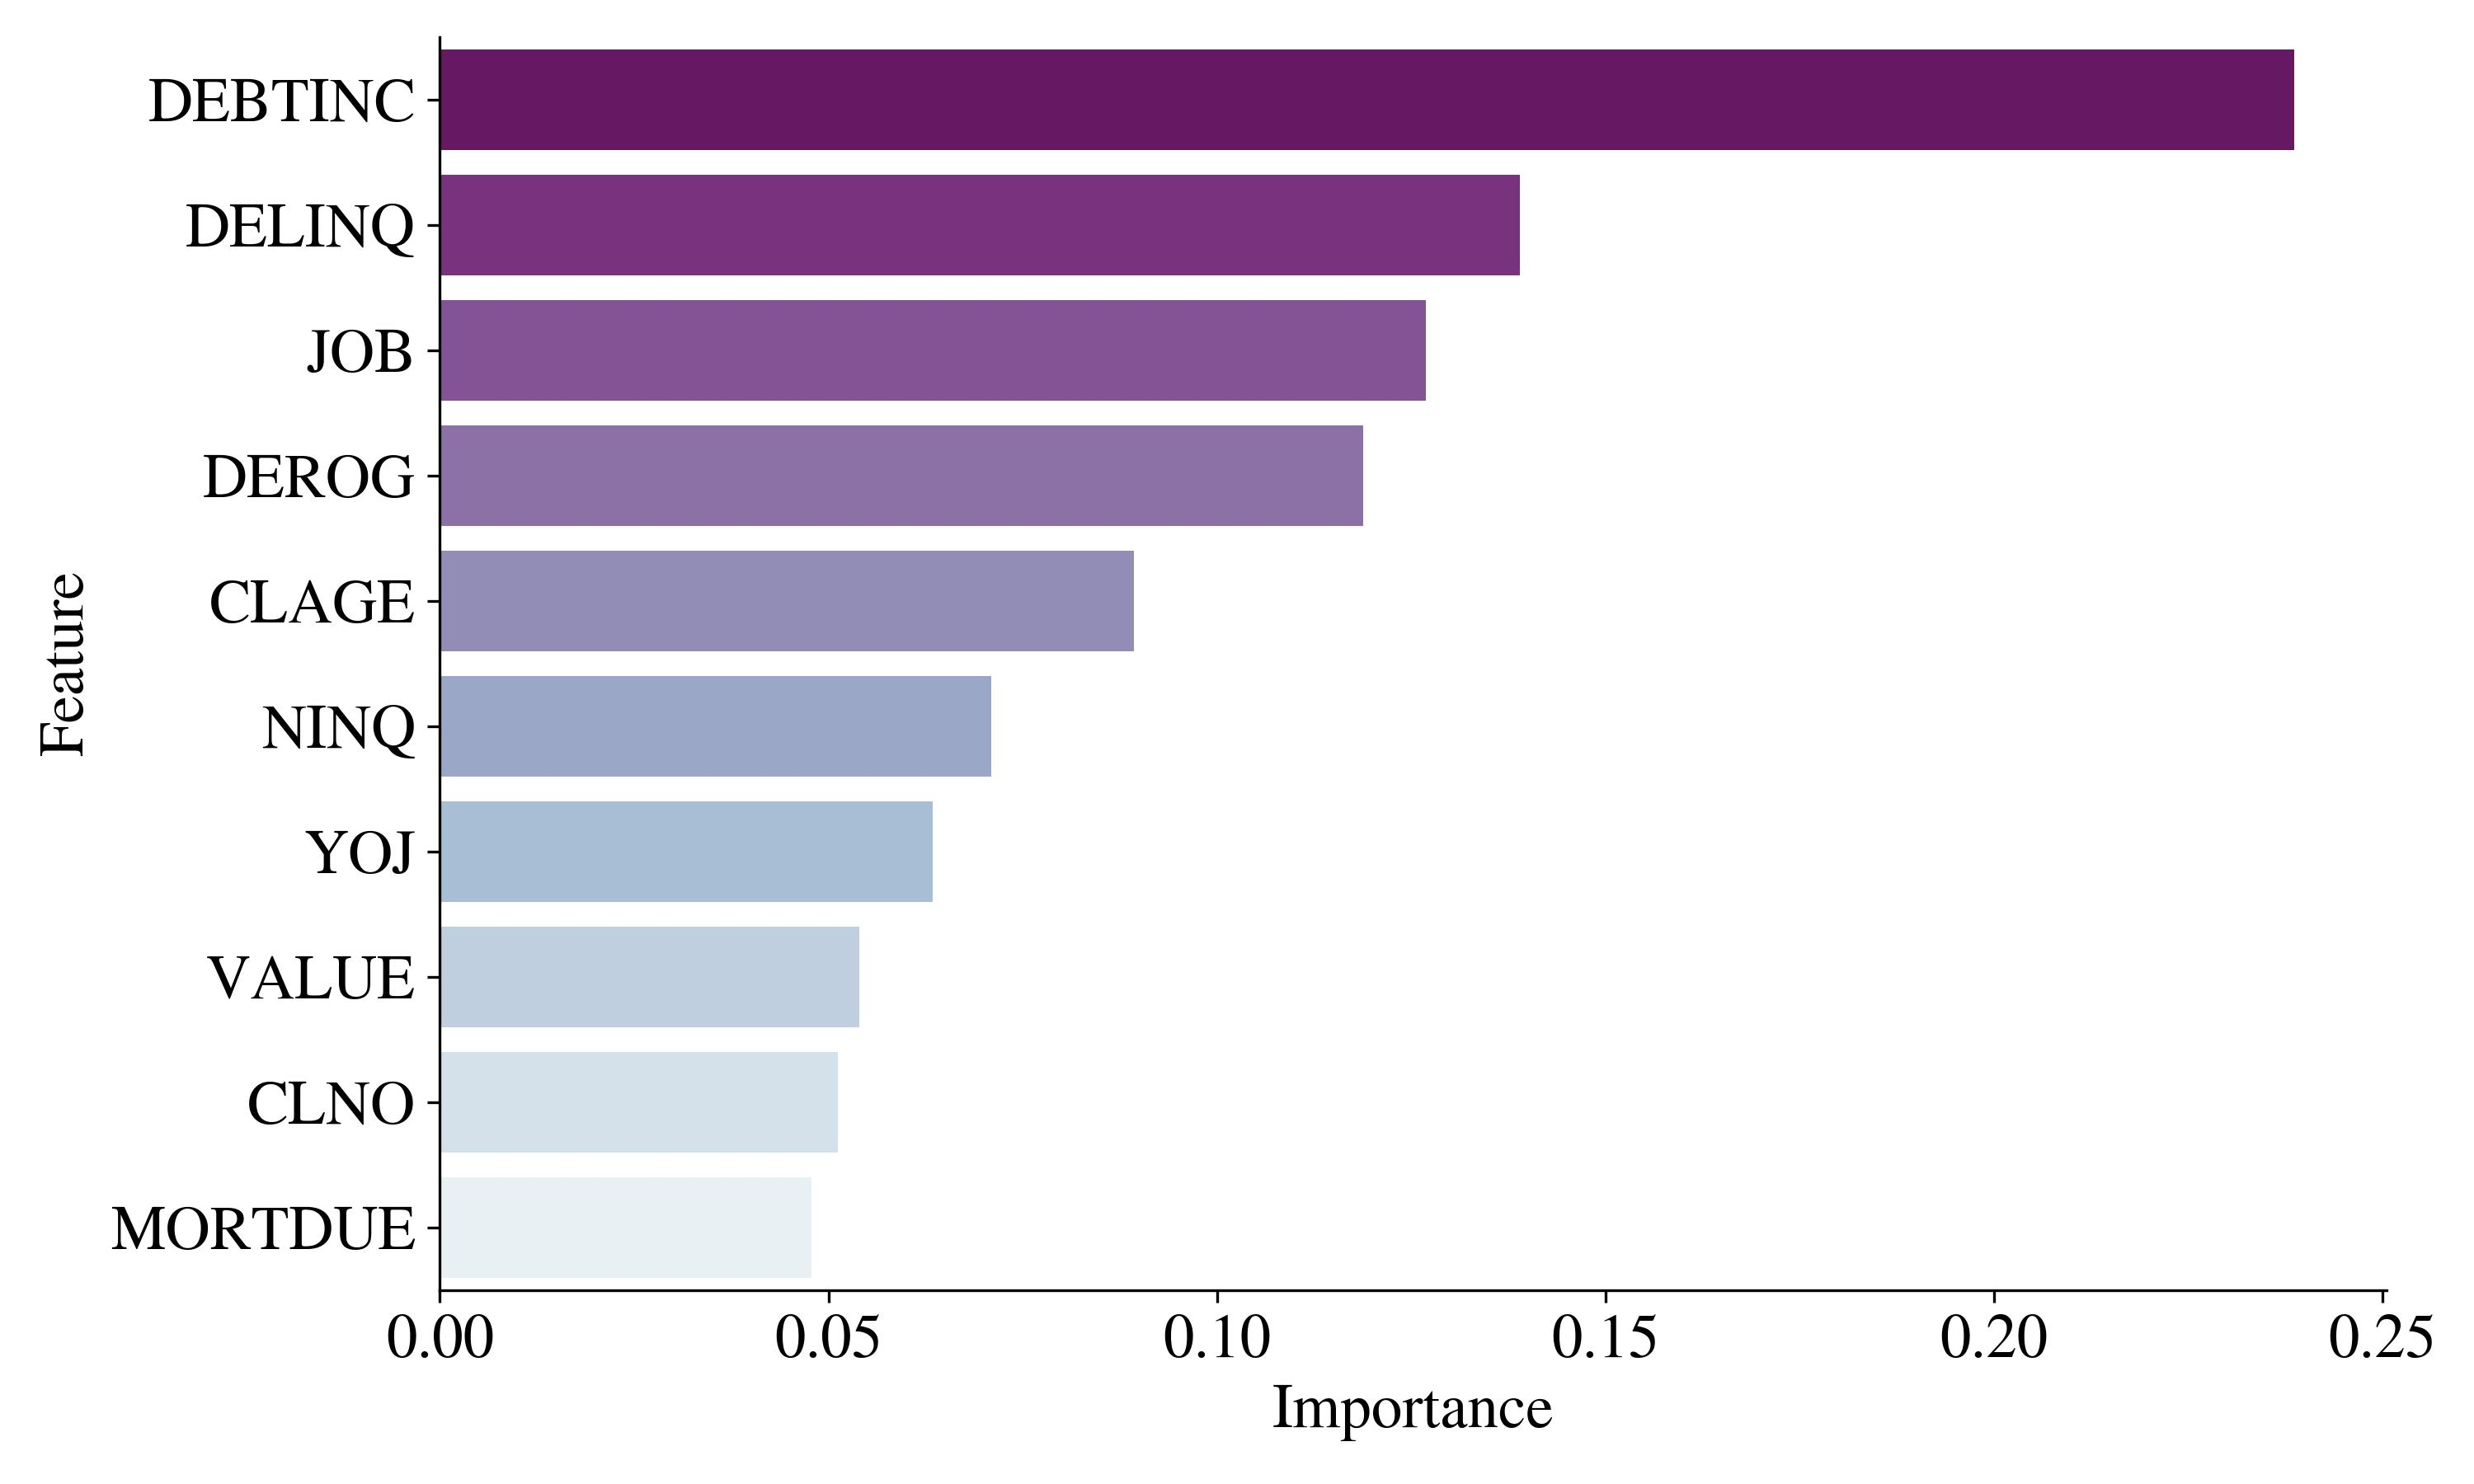
\includegraphics[width=140mm]{Figures/Feature_Importances.jpg}

\centering{\begin{source}Author's results in Python\end{source}}\vspace{-1em}
\end{figure}

Thus, understanding the impact of individual features on model's performance can be useful in identifying areas for improvement, as well as identifying the most significant factors that drive loan defaults.
By focusing on these important features, lenders and policymakers can better understand and address the underlying factors that contribute to default risk, ultimately leading to better lending decisions and improved outcomes for borrowers and lenders alike.


To gain further insights into the impact of the features on the final model's predictions, the SHapley Additive exPlanations (henceforth SHAP) values can be calculated. Particularly, the SHAP value is defined as the mean marginal contribution of each feature value across all possible values in the feature space, while considering feature importance \citep{bhattacharya2022applied}.
The following \autoref{fig:shap} depicts the SHAP summary plot, which provides a clear visualization of the contribution each feature makes to a prediction and the global explainability of the model predictions.
Each dot in the plot represents a feature and its corresponding SHAP value.
The color of the dot represents the feature's value, with red indicating high values and blue indicating low values.
The position of the dot on the x-axis represents the impact of the feature on the prediction, with features on the right-hand side contributing more positively to the prediction, and features on the left-hand side contributing more negatively.

Since our data points are encoded in WoE values, the higher (the more positive) value, the larger the distribution of non-defaulters compared to defaulters, and vice versa, the lower (the more negative) value, the larger the distribution of defaulters compared to non-defaulters.
For the most important features, we can observe that the blue values (negative WoE values) and red values (positive WoE values) are quite separable.
Negative WoE values are positively contributing to the predictions, and positive WoE values are negatively contributing to the predictions. This means that the more negative the WoE value, the more likely the borrower is to default, and vice versa.

Overall, the SHAP summary plot provides a valuable tool for interpreting and understanding the complex decision-making process of the final model.
The plot enables us to examine the impact of individual features on the model's output and helps us identify which features are most influential in the model's decision-making process.
By understanding the relative importance of each feature, we can gain deeper insights into the creditworthiness assessment process and make more informed decisions in the lending industry.

\begin{figure}[H]
\centering
\caption{SHAP Summary Plot}\vspace{0.5em}
\label{fig:shap}\
\includegraphics[width=140mm]{Figures/SHAP_summary_plot.jpg}

\centering{\begin{source}Author's results in Python\end{source}}\vspace{-1em}
\end{figure}


\newpage
\section{Machine Learning Deployment}
\label{sec:deployment}
This section describes the process of taking a trained machine learning model and making it available for use in the real world. It involves taking the model from a development environment and integrating it into a production environment, where it can be used to make predictions or decisions based on new data. In this thesis, the machine learning model is deployed as a web application using Flask and HTML.

\subsection{Final Model Recalibration}
Before deploying the model in a production setting, we undertake the final recalibration of the model using the entire data set, comprising the training, validation, and test sets.
The purpose of this recalibration is to fine-tune the model parameters, thereby maximizing its ability to generalize and yield accurate predictions.

The test set, which has been employed previously during the model evaluation phase, is incorporated into the recalibration process without any risk of data leakage.
By including the test set, the sample size for training is expanded, thereby increasing the model's capacity to generalize effectively.

Upon completion of the recalibration, the final classification threshold for deployment is determined to be \textbf{0.3358}.
We believe that these recalibrated final model's parameters and threshold are optimal for implementation in production settings and will exhibit strong generalization capabilities.


\subsection{Flask and HTML Web Application}
\label{subsec:flaskapp}

In this case, the machine learning model is deployed into a web application using Flask and HTML. The application is temporarily deployed on the Cloud server on the \textbf{PythonAnywhere} platform and is accessible here: \url{http://ml-credit-risk-app-petrngn.pythonanywhere.com/}.
However, the application will be shut down after the thesis defense and will not be available online anymore due to budgetary reasons.
Nevertheless, the code for the application is available in the GitHub repository, and the application can be run locally using any Python compiler.

Furthermore, prior to deployment, we need to prepare several Python inputs for the web application, including:
\begin{itemize}\setlength\itemsep{0em}
\item \textbf{Model} - The final model recalibrated on the training, validation, and test sets.
\item \textbf{Threshold} - The final classification threshold recalibrated on the training, validation, and test sets.
\item \textbf{Features} - The final features used in the final model.
\item \textbf{Data Frame} - The input tabular object used in the web application to store the loan applicant's inputs.
\item \textbf{Optimal Binning Transformator} - Fitted \lstinline{BinningProcess} object for binning and WoE-encoding of the loan applicant's inputs.
\item \textbf{WoE Bins} - Set of bins and WoE values used for mapping the missing values to WoE values.
\item \textbf{LIME explainer} - Fitted \lstinline{LimeTabularExplainer} object for local explainability of the model's prediction.
\end{itemize}


Such inputs required for the machine learning application are exported in the \lstinline{.pkl} format using the \lstinline{dill} module. This format allows for efficient and easy-to-use serialization and deserialization of the inputs. The pickled file is then loaded directly into the Flask application.


For the back-end of the web application, Flask is used to deploy the machine learning model. The Flask application is written in the \lstinline{app.py} file, which is stored in the \lstinline{flask_app} directory. The front-end of the web application is coded in HTML, with CSS and JavaScript elements used to enhance the user interface.


The web application first renders a HTML page, as shown in \autoref{fig:flaskform}.
This page contains a loan application form, in which the user or the loan applicant fills in the respective field values that correspond to the features on which the machine learning model was trained.
The form is designed to capture the necessary information required for the model to make a prediction about the loan applicant's application.
None of the fields in the loan application form need to be filled out. This is because missing values in certain features may indicate a higher risk of default. Conversely, one may choose to impose a restriction on the form, requiring all fields to be filled out. However, this could result in a lower number of received applications from delinquent clients, as they may not have all the necessary information to complete the form.
\begin{figure}[H]
\centering
\caption{Flask Web Application Form}\vspace{0.5em}
\label{fig:flaskform}\
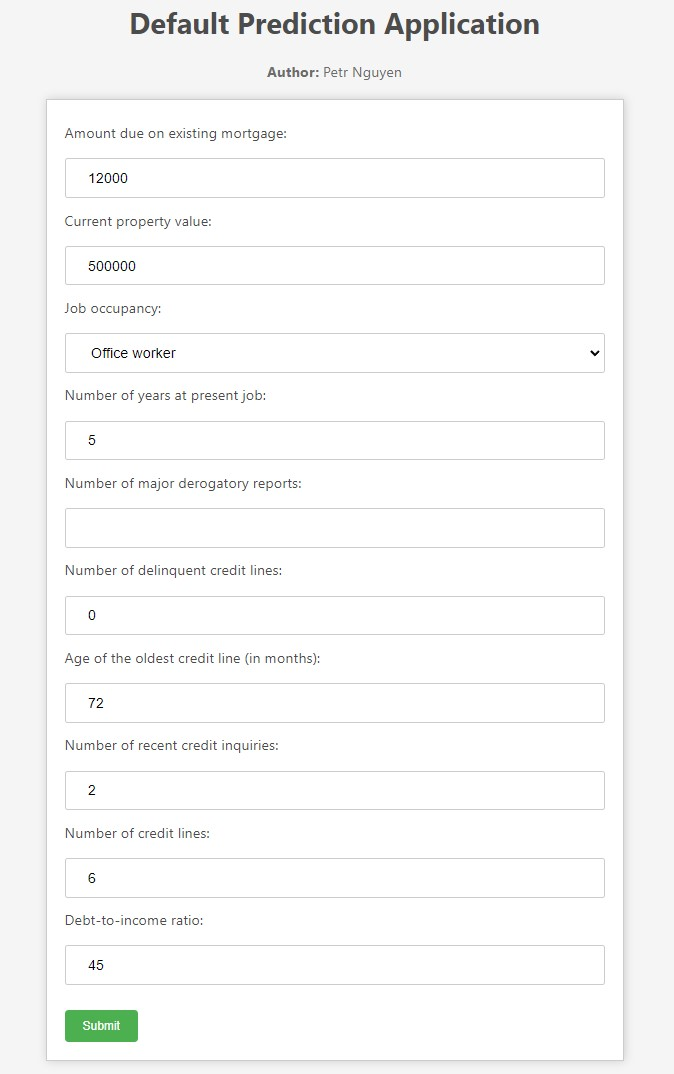
\includegraphics[width=140mm]{Figures/flask_app_form.jpg}

\centering{\begin{source}Author's results in Python\end{source}}\vspace{-1em}
\end{figure}


Once, the loan application form is submitted, the web application uses the pickled input to transform the data from the loan application form and use it in the recalibrated model in order to get the result, whether the given loan applicant would repay his loan based on a predetermined threshold. The result is then displayed in the web application, as shown in \autoref{fig:flaskres}.
Particularly, the web application returns whether the loan application would be denied or approved based on the model's output, and also the probability score of default.

\begin{figure}[H]
\centering
\caption{Flask Web Application - Prediction Result}\vspace{0.5em}
\label{fig:flaskres}\
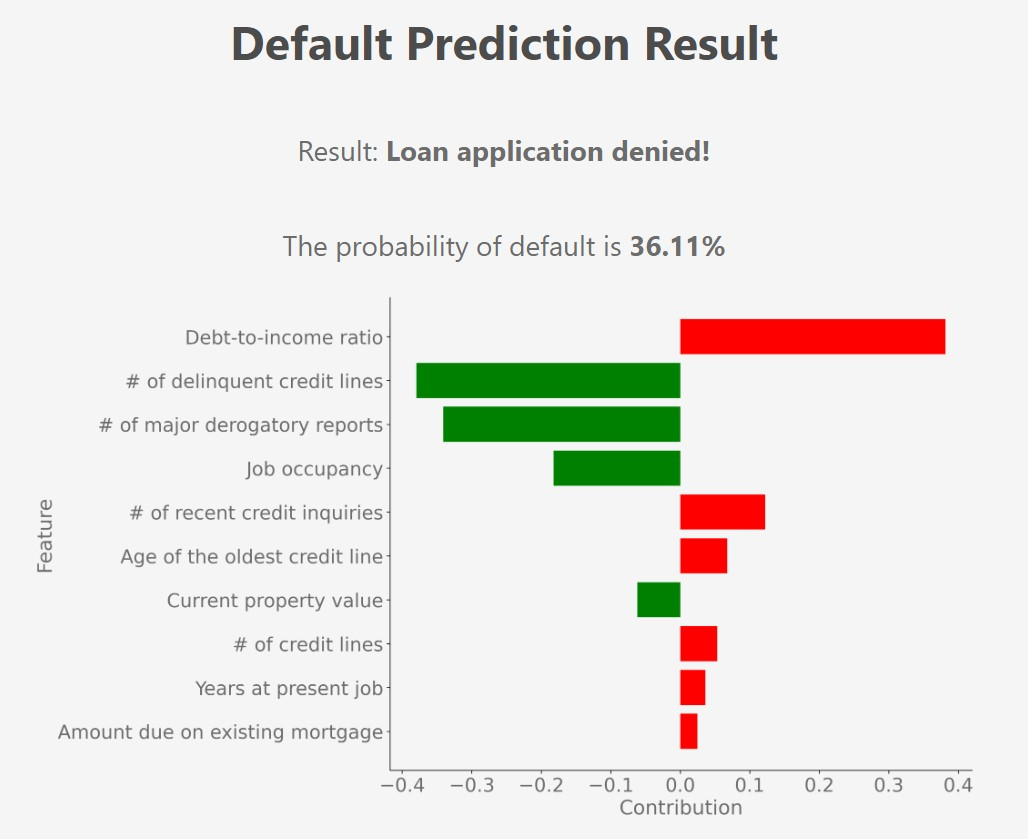
\includegraphics[width=130mm]{Figures/flask_app_result.jpg}

\centering{\begin{source}Author's results in Python\end{source}}\vspace{-1em}
\end{figure}

Besides the prediction results, it also displays the Local Interpretable Model-Agnostic Explanations (henceforth LIME) of the black--box model with respect to the inputs submitted within the form.
LIME focuses on the local explainability of the black box model around the black--box prediction as it generates a new data set consisting of perturbed samples around the given prediction and then trains a surrogate linear model on the new data set.
Such local interpretable, surrogate model should be a good approximation of the black box model in the vicinity of the given prediction, i.e., the local interpretable model is then used to explain the prediction of the black box model \citep{ribeiro2016should}.

The LIME explanation of input instances $x$ is given as follows:
\begin{equation}\label{eq}
\xi(x) = \arg\min_{g \in G} L(f, g, \pi_x) + \Omega(g)
\end{equation}

where $f$ is the original black--box model, $g$ is the surrogate model, $L$ is the loss function measuring how far the explanation $\xi(x)$ is from the prediction produced by the black--box model $f$, and $\Omega(g)$ is the complexity of the surrogate model $g$.


The explanation is given in terms of the feature importance, which is represented by the magnitude of the feature's coefficient in the local interpretable model. The higher the magnitude of the coefficient, the more important the feature is in the prediction of the black box model.
Therefore, as shown in \autoref{fig:flaskres}, the red bars indicate a positive contribution to the probability of default, whereas the green bars indicate a negative contribution to the probability of default. In other words, the features with red bars indicate that the client would probably not repay his loan, and vice versa.
The contributions' magnitudes are in line with the findings from feature importance or SHAP values, which are focused on the global explainability of the black--box model (not local explainability), that features such as debt--to--income ratio (\texttt{DEBTINC}) or number of delinquent credit lines (\texttt{DELINQ}) have the largest impact on the probability of default.
Particularly, a high debt--to--income ratio causes a higher probability of default, whereas no delinquent credit lines lead to a lower probability of default.
